% Generated fragments require trusted human review before compilation.
% This binder never requests shell escape or runs external tools.
\documentclass[11pt]{article}
% Trusted shared apparatus. Requires LuaLaTeX; never use shell escape.
\usepackage{fontspec}
\defaultfontfeatures{Ligatures=TeX}
\IfFontExistsTF{Noto Serif}{\setmainfont{Noto Serif}}{%
  \IfFontExistsTF{DejaVu Serif}{\setmainfont{DejaVu Serif}}{%
    \IfFontExistsTF{Times New Roman}{\setmainfont{Times New Roman}}{%
      \PackageError{gelfand-binder}{No configured Cyrillic serif font installed}{Install Noto Serif or DejaVu Serif, or select an installed Cyrillic font.}%
    }%
  }%
}
\IfFontExistsTF{Noto Sans}{\setsansfont{Noto Sans}}{%
  \IfFontExistsTF{DejaVu Sans}{\setsansfont{DejaVu Sans}}{\setsansfont{Arial}}%
}
\IfFontExistsTF{Noto Sans Mono}{\setmonofont{Noto Sans Mono}}{%
  \IfFontExistsTF{DejaVu Sans Mono}{\setmonofont{DejaVu Sans Mono}}{\setmonofont{Courier New}}%
}
\usepackage[a4paper,margin=22mm]{geometry}
\usepackage{amsmath,amssymb,amsthm,mathtools}
\usepackage{xcolor}
\usepackage{tikz}
\usepackage{tikz-cd}
\usetikzlibrary{arrows.meta,positioning,calc}
\usepackage{hyperref}
\hypersetup{unicode=true,colorlinks=true,linkcolor=blue,pdftitle={Gelfand transcription binder}}
\newtheorem{theorem}{Theorem}
\newtheorem{lemma}{Lemma}
\newtheorem{proposition}{Proposition}
\newtheorem{corollary}{Corollary}
\theoremstyle{definition}
\newtheorem{definition}{Definition}
\newtheorem{example}{Example}
\theoremstyle{remark}
\newtheorem{remark}{Remark}
\setlength{\parindent}{0pt}
\setlength{\parskip}{0.55em}
\setlength{\emergencystretch}{3em}
\newcommand{\SourcePage}[2]{%
  \clearpage\phantomsection\label{#1:source-page}%
  \addcontentsline{toc}{subsection}{#1}%
  {\small\sffamily\color{blue!60!black}Source scan frame: #1; visible page/leaf label: #2}\par\medskip%
}
\newcommand{\Unclear}[3]{%
  \begingroup\color{orange!70!black}%
  [Unresolved reading #1/#2: #3]\endgroup%
}
\newcommand{\Incomplete}[3]{%
  \par\begingroup\color{red!65!black}\textbf{Incomplete #1/#2:} #3\endgroup\par%
}
\newcommand{\SourceFigure}[3]{%
  \par\begingroup\color{blue!60!black}\textbf{\hyperref[#1:source-page]{Source figure #1/#2}:} #3%
  \par\textit{Consult the authoritative scan at this locator.}\endgroup\par%
}



% Reader layout only. Original diplomatic text is retained verbatim.
\setlength{\parskip}{0.35em}
\setlength{\emergencystretch}{4em}
\renewcommand{\SourcePage}[2]{%
  \par\addvspace{1em}\phantomsection\label{#1:source-page}%
  \addcontentsline{toc}{subsection}{#1}%
  {\footnotesize\sffamily\color{blue!55!black}#1%
    \def\givenlabel{#2}\def\nolabel{unlabelled}%
    \ifx\givenlabel\nolabel\else\quad[номер в источнике: #2]\fi
  }\par\nobreak\smallskip%
}
\renewcommand{\Unclear}[3]{%
  \begingroup\color{orange!65!black}%
  \ifmmode\text{[неясно: #3]}\else[неясно: #3]\fi\endgroup%
}
\renewcommand{\Incomplete}[3]{%
  \par\begingroup\color{red!60!black}\textbf{Неразобранный фрагмент:} #3%
  \endgroup\par%
}
\renewcommand{\SourceFigure}[3]{%
  \par\begingroup\color{blue!55!black}\textbf{Рисунок:} #3%
  \par{\small\textit{Исходный рисунок: \hyperref[#1:source-page]{#1}, #2.}}%
  \endgroup\par%
}
\hypersetup{pdftitle={Семинар И. М. Гельфанда. Дипломатическая транскрипция},pdfauthor={},pdfsubject={Русское рабочее издание с отмеченными сомнительными чтениями}}

\usepackage[normalem]{ulem}
\usepackage{newunicodechar}
\usepackage{adjustbox}
\newfontfamily\SourceSymbolFont{Segoe UI Symbol}
\newfontfamily\SourceCJKFont{MS Gothic}
\let\DiplomaticMathUnderline\underline
\renewcommand{\underline}[1]{\ifmmode\DiplomaticMathUnderline{#1}\else\uline{#1}\fi}
\newunicodechar{→}{\ifmmode\text{{\SourceSymbolFont\char"2192}}\else{\SourceSymbolFont\char"2192}\fi}
\newunicodechar{⇒}{\ifmmode\text{{\SourceSymbolFont\char"21D2}}\else{\SourceSymbolFont\char"21D2}\fi}
\newunicodechar{∀}{\ifmmode\text{{\SourceSymbolFont\char"2200}}\else{\SourceSymbolFont\char"2200}\fi}
\newunicodechar{∂}{\ifmmode\text{{\SourceSymbolFont\char"2202}}\else{\SourceSymbolFont\char"2202}\fi}
\newunicodechar{∈}{\ifmmode\text{{\SourceSymbolFont\char"2208}}\else{\SourceSymbolFont\char"2208}\fi}
\newunicodechar{∌}{\ifmmode\text{{\SourceSymbolFont\char"220C}}\else{\SourceSymbolFont\char"220C}\fi}
\newunicodechar{√}{\ifmmode\text{{\SourceSymbolFont\char"221A}}\else{\SourceSymbolFont\char"221A}\fi}
\newunicodechar{∞}{\ifmmode\text{{\SourceSymbolFont\char"221E}}\else{\SourceSymbolFont\char"221E}\fi}
\newunicodechar{∧}{\ifmmode\text{{\SourceSymbolFont\char"2227}}\else{\SourceSymbolFont\char"2227}\fi}
\newunicodechar{∩}{\ifmmode\text{{\SourceSymbolFont\char"2229}}\else{\SourceSymbolFont\char"2229}\fi}
\newunicodechar{∪}{\ifmmode\text{{\SourceSymbolFont\char"222A}}\else{\SourceSymbolFont\char"222A}\fi}
\newunicodechar{∫}{\ifmmode\text{{\SourceSymbolFont\char"222B}}\else{\SourceSymbolFont\char"222B}\fi}
\newunicodechar{∴}{\ifmmode\text{{\SourceSymbolFont\char"2234}}\else{\SourceSymbolFont\char"2234}\fi}
\newunicodechar{∼}{\ifmmode\text{{\SourceSymbolFont\char"223C}}\else{\SourceSymbolFont\char"223C}\fi}
\newunicodechar{≈}{\ifmmode\text{{\SourceSymbolFont\char"2248}}\else{\SourceSymbolFont\char"2248}\fi}
\newunicodechar{≠}{\ifmmode\text{{\SourceSymbolFont\char"2260}}\else{\SourceSymbolFont\char"2260}\fi}
\newunicodechar{≤}{\ifmmode\text{{\SourceSymbolFont\char"2264}}\else{\SourceSymbolFont\char"2264}\fi}
\newunicodechar{≥}{\ifmmode\text{{\SourceSymbolFont\char"2265}}\else{\SourceSymbolFont\char"2265}\fi}
\newunicodechar{⊕}{\ifmmode\text{{\SourceSymbolFont\char"2295}}\else{\SourceSymbolFont\char"2295}\fi}
\newunicodechar{⊗}{\ifmmode\text{{\SourceSymbolFont\char"2297}}\else{\SourceSymbolFont\char"2297}\fi}
\newunicodechar{①}{\ifmmode\text{{\SourceSymbolFont\char"2460}}\else{\SourceSymbolFont\char"2460}\fi}
\newunicodechar{②}{\ifmmode\text{{\SourceSymbolFont\char"2461}}\else{\SourceSymbolFont\char"2461}\fi}
\newunicodechar{③}{\ifmmode\text{{\SourceSymbolFont\char"2462}}\else{\SourceSymbolFont\char"2462}\fi}
\newunicodechar{④}{\ifmmode\text{{\SourceSymbolFont\char"2463}}\else{\SourceSymbolFont\char"2463}\fi}
\newunicodechar{Ⓗ}{\ifmmode\text{{\SourceSymbolFont\char"24BD}}\else{\SourceSymbolFont\char"24BD}\fi}
\newunicodechar{〃}{\ifmmode\text{{\SourceCJKFont\char"3003}}\else{\SourceCJKFont\char"3003}\fi}


% Reader revision 3. Annotation wording and candidates remain unchanged.
\setmainfont{NotoSerif-Regular.ttf}[Path=C:/Windows/Fonts/,ItalicFont=NotoSerif-Italic.ttf,BoldFont=NotoSerif-Bold.ttf,BoldItalicFont=NotoSerif-BoldItalic.ttf]
\usetikzlibrary{shapes.geometric,decorations.pathreplacing,decorations.markings,patterns,fit}
\newsavebox{\ReaderAnnotationBox}
\newcommand{\ReaderAnnotation}[1]{%
  \sbox{\ReaderAnnotationBox}{[неясно: #1]}%
  \ifdim\wd\ReaderAnnotationBox>.70\linewidth
    \parbox[t]{.70\linewidth}{\raggedright[неясно: #1]}%
  \else\usebox{\ReaderAnnotationBox}\fi%
}
\ExplSyntaxOn
\cs_new_protected:Npn \reader_unclear_candidate:n #1
 {
  \tl_set:Nx \l_tmpa_tl { \tl_to_str:n {#1} }
  % Text explicitly guarded inside a mathematical candidate remains math-safe.
  \regex_replace_all:nnN { \\(?:text|textrm|textnormal|textbf|operatorname)\s*\{[^{}]*\} } { } \l_tmpa_tl
  \regex_match:nVTF { [\x{0400}-\x{052F}] | \$ } \l_tmpa_tl
   { \ifmmode \text{\ReaderAnnotation{#1}} \else \ReaderAnnotation{#1} \fi }
   {
    \ifmmode
      [\text{неясно:~}#1]
    \else
      \regex_match:nVTF { [_^] | \\ } \l_tmpa_tl
       { \ensuremath{[\text{неясно:~}#1]} }
       { \ReaderAnnotation{#1} }
    \fi
   }
 }
\RenewDocumentCommand \Unclear { m m m }
 { \begingroup\color{orange!65!black}\reader_unclear_candidate:n{#3}\endgroup }
\ExplSyntaxOff
\newsavebox{\ReaderIncompleteBox}
\newcommand{\ReaderIncompleteNote}[1]{%
 \sbox{\ReaderIncompleteBox}{\textbf{Неразобранный фрагмент:} #1}%
 \ifdim\wd\ReaderIncompleteBox>.70\linewidth
  \parbox[t]{.70\linewidth}{\raggedright\textbf{Неразобранный фрагмент:} #1}%
 \else\usebox{\ReaderIncompleteBox}\fi%
}
\renewcommand{\Incomplete}[3]{%
 \ifmmode\text{\color{red!60!black}\ReaderIncompleteNote{#3}}%
 \else\leavevmode\begingroup\color{red!60!black}\ReaderIncompleteNote{#3}\endgroup\fi%
}
% Ragged right avoids stretching long untranslated abbreviations into margins.
\AtBeginDocument{\raggedright}
\newunicodechar{А}{\ifmmode\text{\char"410\relax}\else\char"410\relax\fi}
\newunicodechar{Б}{\ifmmode\text{\char"411\relax}\else\char"411\relax\fi}
\newunicodechar{В}{\ifmmode\text{\char"412\relax}\else\char"412\relax\fi}
\newunicodechar{Г}{\ifmmode\text{\char"413\relax}\else\char"413\relax\fi}
\newunicodechar{Д}{\ifmmode\text{\char"414\relax}\else\char"414\relax\fi}
\newunicodechar{Е}{\ifmmode\text{\char"415\relax}\else\char"415\relax\fi}
\newunicodechar{Ж}{\ifmmode\text{\char"416\relax}\else\char"416\relax\fi}
\newunicodechar{З}{\ifmmode\text{\char"417\relax}\else\char"417\relax\fi}
\newunicodechar{И}{\ifmmode\text{\char"418\relax}\else\char"418\relax\fi}
\newunicodechar{Й}{\ifmmode\text{\char"419\relax}\else\char"419\relax\fi}
\newunicodechar{К}{\ifmmode\text{\char"41A\relax}\else\char"41A\relax\fi}
\newunicodechar{Л}{\ifmmode\text{\char"41B\relax}\else\char"41B\relax\fi}
\newunicodechar{М}{\ifmmode\text{\char"41C\relax}\else\char"41C\relax\fi}
\newunicodechar{Н}{\ifmmode\text{\char"41D\relax}\else\char"41D\relax\fi}
\newunicodechar{О}{\ifmmode\text{\char"41E\relax}\else\char"41E\relax\fi}
\newunicodechar{П}{\ifmmode\text{\char"41F\relax}\else\char"41F\relax\fi}
\newunicodechar{Р}{\ifmmode\text{\char"420\relax}\else\char"420\relax\fi}
\newunicodechar{С}{\ifmmode\text{\char"421\relax}\else\char"421\relax\fi}
\newunicodechar{Т}{\ifmmode\text{\char"422\relax}\else\char"422\relax\fi}
\newunicodechar{У}{\ifmmode\text{\char"423\relax}\else\char"423\relax\fi}
\newunicodechar{Ф}{\ifmmode\text{\char"424\relax}\else\char"424\relax\fi}
\newunicodechar{Х}{\ifmmode\text{\char"425\relax}\else\char"425\relax\fi}
\newunicodechar{Ц}{\ifmmode\text{\char"426\relax}\else\char"426\relax\fi}
\newunicodechar{Ч}{\ifmmode\text{\char"427\relax}\else\char"427\relax\fi}
\newunicodechar{Ш}{\ifmmode\text{\char"428\relax}\else\char"428\relax\fi}
\newunicodechar{Щ}{\ifmmode\text{\char"429\relax}\else\char"429\relax\fi}
\newunicodechar{Ъ}{\ifmmode\text{\char"42A\relax}\else\char"42A\relax\fi}
\newunicodechar{Ы}{\ifmmode\text{\char"42B\relax}\else\char"42B\relax\fi}
\newunicodechar{Ь}{\ifmmode\text{\char"42C\relax}\else\char"42C\relax\fi}
\newunicodechar{Э}{\ifmmode\text{\char"42D\relax}\else\char"42D\relax\fi}
\newunicodechar{Ю}{\ifmmode\text{\char"42E\relax}\else\char"42E\relax\fi}
\newunicodechar{Я}{\ifmmode\text{\char"42F\relax}\else\char"42F\relax\fi}
\newunicodechar{а}{\ifmmode\text{\char"430\relax}\else\char"430\relax\fi}
\newunicodechar{б}{\ifmmode\text{\char"431\relax}\else\char"431\relax\fi}
\newunicodechar{в}{\ifmmode\text{\char"432\relax}\else\char"432\relax\fi}
\newunicodechar{г}{\ifmmode\text{\char"433\relax}\else\char"433\relax\fi}
\newunicodechar{д}{\ifmmode\text{\char"434\relax}\else\char"434\relax\fi}
\newunicodechar{е}{\ifmmode\text{\char"435\relax}\else\char"435\relax\fi}
\newunicodechar{ж}{\ifmmode\text{\char"436\relax}\else\char"436\relax\fi}
\newunicodechar{з}{\ifmmode\text{\char"437\relax}\else\char"437\relax\fi}
\newunicodechar{и}{\ifmmode\text{\char"438\relax}\else\char"438\relax\fi}
\newunicodechar{й}{\ifmmode\text{\char"439\relax}\else\char"439\relax\fi}
\newunicodechar{к}{\ifmmode\text{\char"43A\relax}\else\char"43A\relax\fi}
\newunicodechar{л}{\ifmmode\text{\char"43B\relax}\else\char"43B\relax\fi}
\newunicodechar{м}{\ifmmode\text{\char"43C\relax}\else\char"43C\relax\fi}
\newunicodechar{н}{\ifmmode\text{\char"43D\relax}\else\char"43D\relax\fi}
\newunicodechar{о}{\ifmmode\text{\char"43E\relax}\else\char"43E\relax\fi}
\newunicodechar{п}{\ifmmode\text{\char"43F\relax}\else\char"43F\relax\fi}
\newunicodechar{р}{\ifmmode\text{\char"440\relax}\else\char"440\relax\fi}
\newunicodechar{с}{\ifmmode\text{\char"441\relax}\else\char"441\relax\fi}
\newunicodechar{т}{\ifmmode\text{\char"442\relax}\else\char"442\relax\fi}
\newunicodechar{у}{\ifmmode\text{\char"443\relax}\else\char"443\relax\fi}
\newunicodechar{ф}{\ifmmode\text{\char"444\relax}\else\char"444\relax\fi}
\newunicodechar{х}{\ifmmode\text{\char"445\relax}\else\char"445\relax\fi}
\newunicodechar{ц}{\ifmmode\text{\char"446\relax}\else\char"446\relax\fi}
\newunicodechar{ч}{\ifmmode\text{\char"447\relax}\else\char"447\relax\fi}
\newunicodechar{ш}{\ifmmode\text{\char"448\relax}\else\char"448\relax\fi}
\newunicodechar{щ}{\ifmmode\text{\char"449\relax}\else\char"449\relax\fi}
\newunicodechar{ъ}{\ifmmode\text{\char"44A\relax}\else\char"44A\relax\fi}
\newunicodechar{ы}{\ifmmode\text{\char"44B\relax}\else\char"44B\relax\fi}
\newunicodechar{ь}{\ifmmode\text{\char"44C\relax}\else\char"44C\relax\fi}
\newunicodechar{э}{\ifmmode\text{\char"44D\relax}\else\char"44D\relax\fi}
\newunicodechar{ю}{\ifmmode\text{\char"44E\relax}\else\char"44E\relax\fi}
\newunicodechar{я}{\ifmmode\text{\char"44F\relax}\else\char"44F\relax\fi}
\newunicodechar{Ё}{\ifmmode\text{\char"401\relax}\else\char"401\relax\fi}
\newunicodechar{ё}{\ifmmode\text{\char"451\relax}\else\char"451\relax\fi}

\newunicodechar{æ}{\ifmmode\text{\char"E6\relax}\else\char"E6\relax\fi}
\newunicodechar{−}{\ifmmode\mathbin{\text{\SourceSymbolFont\char"2212\relax}}\else{\SourceSymbolFont\char"2212\relax}\fi}

\begin{document}
\begin{center}
{\Large Семинар И. М. Гельфанда}\par\medskip
{\LARGE Дипломатическая транскрипция}\par\bigskip
{\large Рабочее русское издание}\par\medskip
{\large Том 32 из 34. Архивная глава 032}\par\bigskip
Кадры GELFAND-P001425 -- GELFAND-P001490\par

\end{center}
\medskip
Сокращения, отменённые записи и сомнительные чтения сохранены.
Неразобранные фрагменты отмечены в тексте. Математические утверждения
источника переданы без молчаливых исправлений.

Это рабочее издание: сверка с рукописью продолжается. В текущем комплекте
учтены 1503 из 1527 кадров; 24 кадра пока представлены явными указателями
отсутствующего возврата. Полный журнал чтений и происхождения данных
сохранён в основном рабочем переплёте.

Границы кадров показаны небольшими синими указателями; печатный текст
продолжается без обязательного разрыва страницы после каждого кадра.
\bigskip\hrule\bigskip
\SourcePage{GELFAND-P001425}{1}
\underline{8/II--88 г.} \underline{Сем. Гельфанда.}

И.М.Г. \underline{Задачи.} 1. Вычислить
\begin{equation*}
(1)\qquad \det\left\Vert\frac{1}{x_i-y_k}\right\Vert_{i,k=1}^{n}.
\end{equation*}
2. Док., что полином Лежандра
\begin{equation*}
\bigl((x^2-1)^n\bigr)^{(n)}
\end{equation*}
имеет только вещественные нули.

3. Может ли ф-я, являющаяся пределом непрерывных функций всюду на отрезке

а) иметь разрывы?

б) иметь всюду плотное м-во точек разрыва?

в) быть всюду разрывной (т.е. в каждой точке)?

4. \textbf{Конформно отобразить на круг}

а)\quad
\begin{adjustbox}{max width=\linewidth}
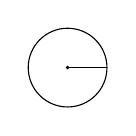
\begin{tikzpicture}[baseline=0cm]
\draw (0,0) circle (0.5);
\fill (0,0) circle (0.025);
\draw (0,0)--(0.5,0);
\end{tikzpicture}
\end{adjustbox}
\quad (круг без радиуса!)

б)
\begin{center}
\begin{adjustbox}{max width=\linewidth}
\begin{tikzpicture}[scale=0.95]
\draw (0.645,0.08) arc (7.07:352.93:0.65)
 -- (3.355,-0.08) arc (187.07:532.93:0.65) -- cycle;
\draw[->] (0,0)--(0.23,0.60);
\node at (-0.10,0.33) {$1$};
\draw[->] (4,0)--(4.58,0.28);
\node at (4.18,0.38) {$1$};
\draw[->] (1.5,0.58)--(1.5,0.08);
\draw[->] (1.5,-0.65)--(1.5,-0.08);
\node at (1.95,0.58) {$10^{-6}$};
\fill (2.25,0) circle (0.025);
\node at (2.52,-0.24) {$A$};
\draw[->] (2.25,-0.18)--(2.25,-1.28);
\draw (2.25,-2.05) circle (0.62);
\draw[->] (2.25,-2.05)--(2.25,-1.43);
\node at (2.07,-1.72) {$1$};
\node at (2.40,-2.08) {$0$};
\node at (4.95,-1.20) {$A\mapsto\text{центр круга}$};
\end{tikzpicture}
\end{adjustbox}
\end{center}

\underline{\textbf{А. Бейлинсон.}} \qquad
\underline{Что нужно знать о теории струн?}

\underline{Конформная теория поля.} \qquad (2-мерная)

Операторное разложение.

Связь с представлениями естественных $\infty$-мерных алгебр Ли.

$W$-алгебры, парафермионы.

[Зачёркнуто: \Unclear{GELFAND-P001425}{vertex-cancellation}{Ве\ldots{} / Вер\ldots{}}]
Алгебра \underline{Вершинных} операторов.
[Начало слова «Вершинных» переписано поверх первоначальных штрихов.]

Различные редукции предст. $\widehat{SL}_2$ к алгебре Вирасоро.

Связь с пространствами модулей алгебро-геометр. структур.

Явные формулы для стат. сумм и
[зачёркнуто: корреляционных функций; над строкой вставлено: корреляторов].

Свойство ветвления характеров.

\SourcePage{GELFAND-P001426}{unlabelled}
\underline{Д. Алексеевский.} \qquad \underline{$G$-структуры}

\underline{Скалярная полевая величина.}

[Зачёркнуто: Поле] — функция от точки $x\in\mathbb{R}^3$ с векторными значениями

(напр. со знач. в $\mathbb{R}$)

\underline{Полевая величина:} зависит от сист. координат

\underline{$G$-структура.}

\underline{Опр. 1}\quad $G\subset GL(V)$, $V=\mathbb{R}^n$.

[Под $G$:] лин. группа.

$G$-структура [вставлено над строкой: на $M^n$] — главное подрасслоение многообразия всех
[зачёркнуто: \Unclear{GELFAND-P001426}{frame-prefix}{ко?}]реперов.

[Справа под «реперов»:] (кореперов) — лучше говорить.

\begin{equation*}
\begin{adjustbox}{max width=\linewidth}
\begin{tikzcd}
M^{(1)} \arrow[r,"GL(V)"] & M
\end{tikzcd}
\end{adjustbox}
\end{equation*}
[Под $M^{(1)}$:] рассл. реперов (главное расслоение)

\begin{equation*}
\begin{adjustbox}{max width=\linewidth}
\begin{tikzcd}
M^{(1)} \arrow[r,"GL(V)"] & M \\
P \arrow[u,phantom,"\cup" description] \arrow[ur,"G"'] &
\end{tikzcd}
\end{adjustbox}
\end{equation*}
$G$ должно действ. на $P$ транзитивно.
\Unclear{GELFAND-P001426}{transitivity}{на $P$ транзитивно}

Тогда это и есть $G$-структура.

\underline{Примеры:} 1) рим. метрика — это $O(V)$-структура

2) Пусть $S$ — тенз. поле, когда оно задаёт $G$-структуру?

Если они все одного кан. вида

(в $\forall$ точке $\exists$ корепер
[зачёркнуто: \Unclear{GELFAND-P001426}{tensor-cancellation}{$\theta$ / $\varphi$?}], прив. $S$ к фикс. виду)

Тогда если $G$ — гр. автоморфизмов кан. вида, то $S$ зад. $G$-структуру.

3) Аффинор зад. $G$-стр., если в $\forall$ точке одинак. жорд. форма

4) Почти компл. структура $J$: $G=GL\left(\frac{n}{2},\mathbb{C}\right)$

5) Почти симпл. структ.: 2-форма $\sigma$ макс. ранга

(симпл. стр.: $d\sigma=0$)

\underline{Опр. 2}\quad $G$-структура — главное $G$-расслоение
$\pi\colon P\overset{G}{\longrightarrow}M$

$G\subset GL(V)$

снабж. векторнозначной 1-формой $\theta\colon TP\to V$,

облад. след. условиями:

\SourcePage{GELFAND-P001427}{2}
а) $G$-эквивариантность

б) $\operatorname{Ker}\theta=T^vP$ (вертик. пр-во), т.е. $\theta$ строго горизонтальна.

\underline{Эквивалентность определений 1 и 2.}

$p\in P$, $x=\pi p$;
\begin{equation*}
\theta_p\colon T_xM\overset{\simeq}{\longrightarrow}V.
\end{equation*}
[Под $T_xM$, со скобкой и стрелкой вниз:]
\Unclear{GELFAND-P001427}{quotient-notation}{$(T_pM/T_p^vM)$}.

[Справа:] это и есть корепер, с к-рым отождествляется точка $p$.

[Зачёркнуто: $\theta_p$ на \Unclear{GELFAND-P001427}{zero-cancellation}{слое?} $0$.]

Корепер $\simeq$ изоморфизм $\theta_p\colon T_xM\overset{\simeq}{\longrightarrow}V$.

$\theta$ наз. \underline{формой смещения}.

Пусть есть $G$-структура
\begin{equation*}
(\pi\colon P\overset{G}{\longrightarrow}M;\theta)
\end{equation*}
Рассм. расслоение 1-струй расслоения $\pi$
\begin{equation*}
\pi'\colon P'\to P
\end{equation*}
$x\to p_x$ — сечение
\begin{equation*}
p'\colon T_xM\to T_{p_x}P
\end{equation*}
\underline{Опр.} 1-струя — отобр. $p'$ — обр. к проекции, $p'=j_x^1(p)$
\begin{equation*}
p'=j_x^1(p)\colon
\begin{adjustbox}{max width=\linewidth}
\begin{tikzcd}
T_xM \arrow[r] & T_{p_x}P \arrow[l,bend left=40]
\end{tikzcd}
\end{adjustbox}
\end{equation*}
т.е. $\pi_*\circ p'=\mathrm{id}$

\underline{Опр.} Горизонтальное подпр-во $H\subset T_pP$
[зачёркнуто: \Unclear{GELFAND-P001427}{horizontal-cancellation}{неразборчиво}]
— такое подпр-во
\begin{equation*}
T_pP=T_p^v\oplus H
\end{equation*}
\underline{Второе опр. 1-струи}

\underline{Элементы $P'$} $=$ \underline{горизонт. подпр-ва}

[Под «Элементы $P'$»:] ($=$ 1-струи)
\begin{equation*}
p'\in P'\quad\Longleftrightarrow\quad H(p')\text{ — горизонт. подпр-во}
\end{equation*}
\underline{Связь:}
\begin{equation*}
p'\colon T_xM\to H(p')\subset T_pP
\end{equation*}
\underline{Опр.} [Зачёркнуто: \Unclear{GELFAND-P001427}{connection-cancellation}{$P'$?}]
$\pi'$ наз. \underline{расслоением связностей};

\SourcePage{GELFAND-P001428}{unlabelled}
\underline{Пр-во связностей:}\quad $\Gamma(\pi')^G$

(т.е. связность — это $G$-эквивар. сечение расслоения $\pi'\colon P'\to P$)

\underline{Связность:}
\begin{equation*}
\begin{aligned}
h\colon P&\to P'\\
p&\mapsto H(p)
\end{aligned}
\end{equation*}
($G$-инв. поле горизонт. подпространств)

Отсюда паралл. перенос (огранич. на кривую)

\underline{Функция кручения}\qquad (аналог структ. констант группы Ли)

Есть вертик. параллелизм:
\begin{equation*}
\begin{aligned}
i_p\colon\mathfrak g&\overset{\simeq}{\longrightarrow}T_p^vP\\
X&\mapsto X_p:=\left.\frac{d}{dt}(\exp tX)p\right|_{t=0}
\end{aligned}
\end{equation*}
\begin{equation*}
\begin{adjustbox}{max width=\linewidth}
\begin{tikzcd}[column sep=small]
p'\in P'\ \Rightarrow\ T_pP={} & T_p^v \arrow[d,"i_p^{-1}"] & {}\oplus H(p') \\
\pi'(p')=p & \mathfrak g &
\end{tikzcd}
\end{adjustbox}
\end{equation*}
[Непосредственно после знака равенства в разложении $T_pP$ зачёркнуто:
\Unclear{GELFAND-P001428}{decomposition-cancellation}{неразборчиво}.]

Возьмём форму $\theta_p\colon T_pP\to V$

и положим
\begin{equation*}
\theta_{H(p')}=\theta|_{H(p')}\colon H(p')\overset{\simeq}{\longrightarrow}V
\end{equation*}
\underline{Опр.}\quad \underline{ф-я кручения} — это отображение
\begin{equation*}
t\colon P'\longrightarrow\operatorname{Hom}(V\wedge V,V)
\end{equation*}
(тензоры типа 1,2)
\begin{equation*}
p'\mapsto t_{p'},\qquad
 t_{p'}(\xi,\eta)=d\theta\bigl(\theta_{H(p')}^{-1}\xi,\theta_{H(p')}^{-1}\eta\bigr)
\end{equation*}
\underline{Свойства ф-и кручения.}

1) $G$-эквивариантность и $G'=\operatorname{Hom}(V,\mathfrak g)$-эквивариантность

\SourcePage{GELFAND-P001429}{3}
\underline{15/II--88 г.}\qquad \underline{Сем. Гельфанда}
(по записям А.К. Звонкина)

В лекциях И.М.Г. о квазилинейных уравнениях (УМН--59, т.14, № 2)
на трёх страницах изложена \underline{вся термодинамика}.

\underline{Конкр. зад. по геометрии:} что такое угол между двумя 2-мерными подпр-вами
в 4-мерном пр-ве?

Угол — инвариант относит. дв-ния (для прямых).

Есть 2 варианта: для ориентир. прямых и для неориентированных.

Для плоскостей: сколько этих инвариантов и каковы они?

\underline{Вопрос:} найти все инварианты двух подпространств гильбертова пространства.

[Зачёркнуто: \Unclear{GELFAND-P001429}{speaker-cancellation}{Зам\ldots{}?}]

\underline{Замолодчиков Саша.}\qquad
\underline{Конформная (2-мерная) теория поля.}

\begin{equation*}
\langle A_1(x_1)A_2(x_2)\ldots A_N(x_N)\rangle,\quad x_i\in\mathbb{R}^2;
\tag{1}
\end{equation*}
— «корреляционные функции»

$\mathcal A\ni A$ — поля (вообще говоря, $\infty$-мерное)

(1) — $N$-линейная ф-я на пр-ве полей $\mathcal A$
(к тому же ф-я от $(x_1,\ldots,x_N)$)

Уточним понятие среднего в (1):
\begin{equation*}
(1)=Z^{-1}\int\mathcal D\varphi\,e^{-S[\varphi]}A_1(x_1)\ldots A_N(x_N),
\tag{2}
\end{equation*}
где $\varphi=\varphi(x)$,
\begin{equation*}
S=\int\sigma\bigl(\varphi(x),\partial\varphi(x)\bigr)\,dx,
\tag{3}
\end{equation*}
\begin{equation*}
Z=\int\mathcal D\varphi\,e^{-S[\varphi]}
\tag{4}
\end{equation*}
[Номер (4) переписан поверх \Unclear{GELFAND-P001429}{equation-number}{3?}.]

\underline{Свойства корреляционных функций.}

1) «Алгебра полей»

Пусть поля образуют ассоц. алгебру;
[зачёркнуто: \Unclear{GELFAND-P001429}{algebra-cancellation}{неразборчиво}]
с \Unclear{GELFAND-P001429}{algebra-ending}{образующими / образующих} $A_i(x)$.
[Над строкой вставлено: (с континуумом); окончание слова «образующими» исправлено.]

Пусть $\{A_i\}$ — базис в $\mathcal A$. Тогда
\begin{equation*}
A_i(x)A_j(y)=\sum_k c_{ij}^k(x,y)A_k(y)
\end{equation*}
[К $c_{ij}^k(x,y)$ проведена стрелка от подписи:] числовые ф-и от $x,y$

Положим
\begin{equation*}
\langle A_k(x)\rangle=a_k(x)
\end{equation*}

\SourcePage{GELFAND-P001430}{unlabelled}
(Знания функций $c_{ij}^k$ и $a_k$ достаточно для вычисления корреляц.
функций: заменяем пару $A_1A_2$ на $\sum c^kA_k$ и т.д.)

2) \underline{«Инвариантность»}

Рассм. поле $T$ вида
\begin{equation*}
T^{\mu\nu},\quad\mu,\nu=1,2;\quad T^{\mu\nu}\in\mathcal A.
\end{equation*}
Кстати
\begin{equation*}
\frac{\partial}{\partial x^\mu}A_i(x)A_j(y)
=\sum\frac{\partial}{\partial x^\mu}c_{ij}^k(x,y)A_k
\tag{5}
\end{equation*}
\begin{equation*}
\frac{\partial T^{\mu\nu}}{\partial x^\mu}=0
\tag{6}
\end{equation*}
Рассм. [зачёркнуто: \Unclear{GELFAND-P001430}{integral-cancellation}{оператор?}] интеграл
\begin{equation*}
\oint T^{\mu\nu}(x)A(y)\,\varepsilon_{\mu\lambda}\,dx^\lambda
\tag{7}
\end{equation*}
[Индекс $\lambda$ у $\varepsilon$ переписан поверх
\Unclear{GELFAND-P001430}{epsilon-first-index}{$\nu$?}.]

[Справа от интеграла:]
\begin{center}
\begin{adjustbox}{max width=\linewidth}
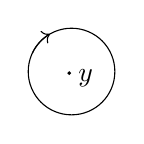
\begin{tikzpicture}
\draw (0,0) circle (0.55);
\draw[->] (155:0.55) arc (155:120:0.55);
\fill (-0.03,-0.02) circle (0.025);
\node at (0.18,-0.08) {$y$};
\end{tikzpicture}
\end{adjustbox}
\end{center}
[Выносная подпись к $\varepsilon$ в (7):]
\begin{equation*}
\varepsilon_{\mu\lambda}=-\varepsilon_{\lambda\mu},\qquad\varepsilon_{12}=1
\end{equation*}
Он определяет линейный оператор в $\mathcal A$.

\underline{Требуется:} $\exists$ поле $T$ такое, что этот оператор равен $\dfrac{\partial}{\partial y}$.

$T^{\mu\nu}:=$ «тензор энергии-импульса»
\begin{equation*}
\oint T^{\mu\nu}(x)A_i(y)\,
\varepsilon_{\mu\nu}
\,dx^\lambda
=\frac{\partial}{\partial y^\nu}A_i(y)
\end{equation*}
\Unclear{GELFAND-P001430}{epsilon-repeat}{$\varepsilon_{\mu\nu}$}
$1')$\quad $c_{ij}^k(x,y)=c_{ij}^k(x-y)$ — функции одной переменной в $\mathbb R^2$.

3) \underline{«Условие положительности»}

$A\mapsto A^+\in\mathcal A$ — инволюция.
\begin{equation*}
A_i^+(x)A_j^+(y)=\sum\overline{c}_{ij}^k(\widetilde x-\widetilde y)A_k^+(y)
\tag{8}
\end{equation*}
\begin{equation*}
x=(x^1,x^2)\quad\Rightarrow\quad\widetilde x=(-x^1,x^2)
\end{equation*}
\underline{Требование:} матрица $\langle A_i^+(\widetilde x)A_j(x)\rangle$
положительно определена для всех $x$.

\underline{Задача} состоит в том, чтобы строить содержательные примеры всего этого.

\SourcePage{GELFAND-P001431}{4}
Введём в $\mathbb R^2$ комплексные координаты
\begin{equation*}
z=x^1+ix^2\qquad ds^2=dz\,d\bar z
\end{equation*}
\begin{equation*}
T^{\nu\mu}=T^{\mu\nu}
\tag{9}
\end{equation*}
\begin{equation*}
\left.\begin{aligned}
T&=T^{zz},\quad\bar T=T^{\bar z\bar z}\\
\Theta&=T^{z\bar z}=0
\end{aligned}\right\}
\quad\begin{gathered}
\text{при этих дополнительных условиях}\\
\text{теория наз. «конформной теорией поля»}
\end{gathered}
\tag{10}
\end{equation*}
\Unclear{GELFAND-P001431}{tensor-components}{$T=T^{zz},\ \bar T=T^{\bar z\bar z}$}

[Стрелка снизу к $\Theta=0$:] Важн. частный случай: безмассовая теория

\underline{Контр. вопрос:} записать $T^{zz}$, $T^{z\bar z}$, $T^{\bar z\bar z}$ через $T^{\mu\nu}$

(это задача линейной алгебры)
\begin{equation*}
\frac{\partial T}{\partial\bar z}=0,\quad
\frac{\partial\bar T}{\partial z}=0
\qquad\text{— уравнения Коши--Римана}
\tag{11}
\end{equation*}
\begin{equation*}
\Updownarrow
\end{equation*}
$T$ — аналитическая функция $z$, $T=T(z)$, $\bar T=\bar T(\bar z)$.
\begin{equation*}
T(z)A_i(z_1,\bar z_1)=\sum f_{ij}(z-z_1)A_j(z_1,\bar z_1)
\tag{12}
\end{equation*}
\underline{В электродинамике:}

$\psi$ — электрон

$A$ — фотон
\begin{equation*}
\{A_i\}=\{\psi,\psi^2,\psi\partial\psi,\ldots,A,A^2,A\psi,\ldots\}
\end{equation*}
$\psi^4$ ещё есть, но $\psi^5=\psi^6=0$ (т.к. всего у спинора 4 компоненты)

у $A$ есть все степени

Но, вообще говоря, $A^2$ не существует.

Не надо брать поля в одной точке, надо в разных.
\begin{equation*}
\oint\frac{dz}{2\pi i}\,z^{n+1}T(z)A_i(z_1,\bar z_1)
=L_nA_i(z_1,\bar z_1)
\tag{13}
\end{equation*}
[Справа от (13):]
\begin{center}
\begin{adjustbox}{max width=\linewidth}
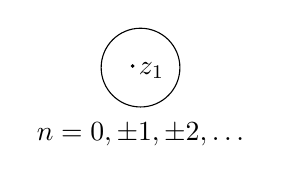
\begin{tikzpicture}
\draw (0,0) circle (0.5);
\fill (-0.10,0.02) circle (0.025);
\node at (0.14,-0.04) {$z_1$};
\node at (0,-0.85) {$n=0,\pm1,\pm2,\ldots$};
\end{tikzpicture}
\end{adjustbox}
\end{center}
\begin{equation*}
L_{-1}=\frac{\partial}{\partial z_1}
\end{equation*}
\begin{equation*}
\bar T(\bar z)\to\bar L_n;\quad
\bar L_{-1}=\frac{\partial}{\partial\bar z_1}
\tag{14}
\end{equation*}
$T(z_1)T(z_2)$ — ф-я от $z_1$, аналитическая везде, кроме точки $z_2$;
разложим её в ряд Лорана.

\SourcePage{GELFAND-P001432}{unlabelled}
\begin{equation*}
T(z_1)T(z_2)=\sum_{m=-\infty}^{\infty}(z_1-z_2)^m T_m(z_2),\quad T_m\in\mathcal A
\tag{15}
\end{equation*}
Сделаем предположение:
\begin{equation*}
(15)=(z_1-z_2)^{-4}T_{-4}+(z-z_2)^{-3}T_{-3}+\ldots
\tag{16}
\end{equation*}
\Unclear{GELFAND-P001432}{laurent-factor}{$(z-z_2)^{-3}$}

(т.е. ряд обрывается внизу на члене $-4$)
\begin{equation*}
T_{-1}=\frac{dT}{dz_2}(z_2)
\tag{17}
\end{equation*}
\begin{equation*}
T_{-2}=2T(z_2)\quad\leftarrow\quad
\text{выводится из того, что $T$ — тензор 2-го ранга}
\tag{18}
\end{equation*}
Важнее всего определить самые сингулярные слагаемые: $T_{-3}$ и $T_{-4}$.

Из условия положительности следует, что
\begin{equation*}
T_{-4}\sim\text{единичн. оператор:}\quad T_{-4}=\frac c2,\quad T_{-3}=0
\tag{19}
\end{equation*}
\begin{equation*}
T(z)T(z')=\frac{c}{2(z-z')^4}+\frac{2T(z')}{(z-z')^2}
+\frac{1}{z-z'}T'(z')+\ldots
\tag{20}
\end{equation*}
[Стрелка к многоточию в (20):] дальнейшие члены не интересны

Из этого разложения получаем
\begin{equation*}
\fbox{$[L_n,L_m]=(n-m)L_{n+m}+\frac{c}{12}(n^3-n)\delta_{n+m,0}$}
\tag{21}
\end{equation*}
Это соотн. \underline{алгебры Вирасоро} (центр. расширение алгебры векторных полей на окружности)

(В обычной квантовой механике — алгебра Ли группы параллельных переносов на прямой: $\frac{d}{dx}$ — малый перенос — импульс)

Вообще тензор энергии-импульса получается из преобразований координат

В этом смысле квантовую механику придумал Софус Ли: он первый заменил преобразования координат на беск. малые преобразования.

(Для алгебры Вирасоро группой служит группа диффеоморфизмов окружности.)

Длины меньше $10^{-31}$ см не имеют смысла — это утверждение уже не зависит
[зачёркнуто: \Unclear{GELFAND-P001432}{lower-cancellation}{от / не}]
ни от какой теории — из соотношений между универсальными константами.

\SourcePage{GELFAND-P001433}{5}
$p$-адическая теория имеет вычислительные преимущества: некоторые детерминанты лучше всего считать адельным способом

Но есть и ещё одно: физика ничего не может сказать не только о далёких точках, но и о близких.

[Следующий абзац выделен двумя вертикальными чертами слева:]
О двумерных многообразиях всё известно, но о трёхмерных и четырехмерных известно столь же мало, как и 2000 лет назад

Это новая комбинаторика.

Как придумать, что такое пространство, если есть запрет на малые расстояния? Не хватает воображения. (Толщина; дискретность; искривления;\ldots)

[Короткая горизонтальная черта.]

Конформная инвариантность: теория не меняется при замене
\begin{equation*}
\begin{cases}
z\mapsto z+\varepsilon(z)\\
\bar z\mapsto\bar z+\bar\varepsilon(\bar z)
\end{cases}
\tag{22}
\end{equation*}
Взяв $\varepsilon(z)\sim z^{n+1}$, получим алгебру Вирасоро

Выясним, как меняется среднее
\begin{equation*}
\langle A_1(x_1)\ldots A_N(x_N)\rangle
=Z^{-1}\int A_1(x_1)\ldots A_N(x_N)e^{-S[\varphi]}\mathcal D\varphi
\tag{23}
\end{equation*}
при заменах
\begin{equation*}
x^\mu\to x^\mu+\varepsilon^\mu(x)
\tag{24}
\end{equation*}
Вариация
\begin{equation*}
\begin{aligned}
\delta\langle A_1(x_1)\ldots A_N(x_N)\rangle
&=\sum_{k=1}^{N}\langle A_1\ldots\delta_\varepsilon A_k\ldots A_N\rangle\\
&\quad+\int\partial_\mu\varepsilon_\nu
\langle T^{\mu\nu}(x)A_1\ldots A_N\rangle\,d^2x=0
\end{aligned}
\tag{25}
\end{equation*}
перебросим (по частям) $\partial_\mu$ на $T^{\mu\nu}$ и воспольз. $\partial_\mu T^{\mu\nu}=0$;

интегрир. по маленьким контурам, окруж. $x_1,\ldots,x_N$, получим
\begin{equation*}
\delta_\varepsilon A_k(y)=\oint_{c_y}\varepsilon_\nu(x)T^{\lambda\nu}(x)
\varepsilon_{\lambda\mu}\,dx^\mu A_k(y),
\end{equation*}
но
\begin{equation*}
\partial_\mu\varepsilon_\nu+\partial_\nu\varepsilon_\mu=\delta_{\mu\nu}\rho(x);
\end{equation*}
\Unclear{GELFAND-P001433}{conformal-factor}{$\rho(x)$ / $g(x)$}

$T^{z\bar z}=T^\mu_\mu$ — след; $=0$.
\Unclear{GELFAND-P001433}{trace-equality}{$T^{z\bar z}=T^\mu_\mu$}

[Внизу справа:]
\begin{center}
\begin{adjustbox}{max width=\linewidth}
\begin{tikzpicture}
\node[align=left] at (0,0) {Что\\получилось};
\draw (1.7,0) ellipse (0.35 and 0.45);
\node at (1.7,0) {?};
\end{tikzpicture}
\end{adjustbox}
\end{center}

\SourcePage{GELFAND-P001434}{unlabelled}
Поля классифицируются по представлениям алгебры Вирасоро.
\begin{equation*}
\left\{\begin{aligned}
L_n\phi_\alpha&=0,\quad n>0;&\qquad\bar L_n\phi_\alpha&=0;\\
L_0\phi_\alpha&=\Delta_\alpha\phi_\alpha;&\qquad
\bar L_0\phi_\alpha&=\bar\Delta_\alpha\phi_\alpha;
\end{aligned}\right.
\tag{26}
\end{equation*}
\begin{equation*}
L_{n_N}\ldots L_{n_1}\phi_\alpha=[\phi_\alpha]
\end{equation*}
\Unclear{GELFAND-P001434}{descendant-bracket}{$L_{n_N}\ldots L_{n_1}\phi_\alpha=[\phi_\alpha]$}
\begin{equation*}
n_i<0;\quad\Delta_\alpha,\bar\Delta_\alpha\text{ — два числа }\geq0
\end{equation*}
\begin{equation*}
\mathcal A=\bigoplus_\alpha[\Phi_\alpha]
\end{equation*}
\begin{equation*}
\mathrm I\in\mathcal A;\qquad\mathrm I\cdot A_i(x)=A_i(x),\quad
\text{для него }\Delta,\bar\Delta=0
\end{equation*}
\begin{equation*}
\begin{gathered}
z\to\lambda z\\
\bar z\to\bar\lambda z
\end{gathered}
\qquad\phi_\alpha\to\lambda^{\Delta_\alpha}\bar\lambda^{\bar\Delta_\alpha}\phi_\alpha,
\end{equation*}
\Unclear{GELFAND-P001434}{barred-coordinate}{$\bar z\to\bar\lambda z$}
\begin{equation*}
\Delta_\alpha-\bar\Delta_\alpha=S_\alpha\text{ — спин }\phi_\alpha.
\end{equation*}


\SourcePage{GELFAND-P001435}{10}
\Unclear{GELFAND-P001435}{heading-date}{22.2.88 / 22.2.82}
\underline{Углы между подпространствами.}

\begin{center}
\underline{Серия задач про углы между подпространствами}

(\underline{И.М. Гельфанд}; по записям А.К. Звонкина)
\end{center}

Нек-рые доступны 8-класснику (задачи в $R^2$ и $R^3$),
другие для доктора наук (задачи в гильб. пр-ве).

Что такое «угол» между двумя прямыми на плоскости?
Это ортогональный инвариант этой пары прямых — т.е. некая
числовая хар-ка, к-рая не меняется при всех ортогональных преобр.
плоскости.

Более того, угол — это \underline{полная система инвариантов}, т.е.
пара прямых тогда и только тогда переводится в другую пару
ортог. пр-ем, когда у этих двух пар прямых одинаковый угол.

В дальнейшем под «углом» понимается полная система
инвариантов нек-рого объекта под действием нек-рой группы.
Иногда это число, иногда — конечное или счетное мн-во чисел,
иногда даже континуум чисел.

(В случаях, когда речь будет идти, скажем, о четверке подпр-в
$\Rightarrow$ [стрелка продолжения строки]
лин. пр-ва, не будем употреблять выражение «\underline{угол между\ldots}»,
т.к. непонятно, между чем?, а будем говорить «\underline{угол для\ldots}».)

Во всех задачах представляет интерес не только то,
\underline{что такое угол}, но также и \underline{какие значения он может
принимать}.

\paragraph*{I. \underline{Задачи для школьников.}}
1. Что такое угол между прямой и плоскостью в трёхмерном
пр-ве.

(Два варианта: прямая ориентирована и не ориентирована).

2. Что такое угол между двумя плоскостями в трёхмерном
пространстве?

\paragraph*{II. \underline{Задачи для студентов.}}
3. Дано 4-мерное линейное пр-во со скал. произведением.
(не $R^4$, т.к. не выделены оси). Что такое угол между двумя его
двумерными подпространствами?

4. Дано $\{L,(\cdot,\cdot)\}$, $\dim L=n$, $v\in L$, $V\subset L$,
$\dim V=k$.

Определить угол между $v$ и $V$.

\SourcePage{GELFAND-P001436}{unlabelled}
5. Дано $\{L,(\cdot,\cdot)\}$, $\dim L=n$, $V,W\subset L$,
$\dim V=k$, $\dim W=m$. Определить угол между $V$ и $W$.

6. Пусть $L$ — просто линейное пространство (без скалярного
произведения). Определить угол для

(а) подпространства $L$

(б) пары подпространств

(в) тройки подпространств.

(Под группой здесь надо понимать $GL(n)$)

7. Дана плоскость Минковского, т.е. $L$, $\dim L=2$
с незнакоопределенным скалярным произведением $-x_1^2+x_2^2$.
Определить угол между двумя прямыми (т.е. инвариант
относительно группы преобразований, сохраняющих это
скалярное произведение).

8. Дальнейшие вариации:
\begin{itemize}
\item[—] для пространства Минковского более высокой размерности
и двух его подпространств
\item[—] для других пространств с неопределенной метрикой
(т.е. когда в скалярном произведении более чем один минус)
\item[—] для пространств с вырожденной формой (например, $R^3$
со скалярным произведением $x_1^2+x_2^2$).
\end{itemize}

Для всех перечисленных задач надо рассмотреть случаи
групп $O(n)$ и $SO(n)$.

\paragraph*{III. \underline{Задачи для аспирантов.}}
9. Дано лин. пр-во $L$ и четверка его подпр-в. Найти угол
этой четверки (это содержание работы Гельфанда и Пономарева)

10. (А.А. Кириллов-младший) Дано $\{L,(\cdot,\cdot)\}$; тогда в тензорных
степенях $L$ тоже определено скалярное произведение. Пусть
$a,b\in L\otimes L$. Найти угол между подпространствами $a\otimes L$ и
$L\otimes b$, вложенными в $L\otimes L\otimes L$.

(Это нужно для алг-р Гекке и ур-я Яна-Бакстера)

\SourcePage{GELFAND-P001437}{11}
\paragraph*{IV. \underline{Задачи для кандидатов и док-торов наук.}}
11. Определить угол для двух подпр-в гильбертова пр-ва.
Привести примеры, когда значением угла является счётное
мн-во чисел, и когда — континуум чисел.

12. Та же задача для гильбертова пр-ва с неопределенной метрикой.

\paragraph*{\underline{Комментарии.}}
1. В этих задачах особенно трудна вторая часть; например,
если дано подпр-во и угол, а требуется построить
другое подпр-во, лежащее под данным углом к данному.

2. Линейный оператор можно задавать с помощью
четверки подпространств.

\SourcePage{GELFAND-P001438}{unlabelled}
\underline{21/III-88} \qquad \underline{Сем. Гельфанда}

\underline{\underline{Радул А.}}

\paragraph*{\underline{Квантовые скобки Гельфанда — Дикого}}
(по С. Лукьянову) \qquad Рассм. на $S^1$ оператор
\begin{equation*}
L=\partial_z^N+\sum_{i=0}^{N-1}u_{N-1}(z)\partial_z^i . \tag{1}
\end{equation*}
\Unclear{GELFAND-P001438}{operator-coefficient}{Индекс коэффициента: $N-1$ / $N-i$.}

и пр-во ф-лов вида
\begin{equation*}
f[u]=\oint P\bigl[z,u_i^{(k)}(z)\bigr]dz \tag{2}
\end{equation*}
и их конечных произведений; $P$ — полином по $u_i^{(k)}$.

На таких ф-лах определены 2 скобки Гельфанда — Дикого
\begin{equation*}
\frac{\delta f}{\delta u_i}\quad
\text{опр. из соотн.:}\quad
\left.\frac{d}{d\varepsilon}f[u+\varepsilon\delta u]\right|_{\varepsilon=0}
=\oint dz\,\frac{\delta f}{\delta u_i}\delta u_i . \tag{3}
\end{equation*}

\underline{И.М. Гельфанд}
\paragraph*{\underline{Отступление о функциональном анализе}}
Вся интуиция функц. анализа исходила из того, что ф-лы — это тоже
ф-и, но на $\infty$-мерном пр-ве.

И.М.Г. изменил свою точку зрения и отсюда два следствия.

1) Бывают ф-лы разных типов и их надо классифицировать.

2) Ф-лы — не ф-и $\Rightarrow$ влияет на геометрию.

1) В вар. исчислении бывают ф-лы
\begin{equation*}
\int_0^L f\bigl(x,u(x),u'(x)\bigr)\,dx \tag{*}
\end{equation*}
\Unclear{GELFAND-P001438}{local-functional-argument}{Аргумент среднего $u$: $x$ / $z$.}

Это ф-л от $u$, но он обладает св-вом:

\SourceFigure{GELFAND-P001438}{locality-diagram}{Наклонная линия с двумя выступами вверх; подписи и стрелки не видны. В вершинах выступов есть разрывы штрихов.}

если есть приращ. [вставлено над строкой, со стрелкой к этому месту: $u$]
в 2-х местах, то
приращ. ф-ла (*) будет суммой
[зачеркнуто: \Unclear{GELFAND-P001438}{locality-cancelled}{2 / начало «двух»?}]
приращений

(локальность!)

\underline{\Unclear{GELFAND-P001438}{general-functional-phrase}{5-й возм. обобщ. ф-й: / Б-й возм. обобщ. ф-й:}}
отсюда вытекает
(и из непрерывности),
что тогда [зачеркнуто: \Unclear{GELFAND-P001438}{general-functional-cancelled}{от / он}]
ф-л имеет такой вид

[зачеркнутый знак: \Unclear{GELFAND-P001438}{type-zero-cancelled}{1 / И}]
Это 0-й тип.

\SourcePage{GELFAND-P001439}{27}
\underline{1-й тип:} если
\begin{equation*}
\frac{\delta}{\delta u}F(u)\quad\text{\underline{локален}.}
\end{equation*}
Таковы ф-лы, встр. в теории Атьи-Зингера

Беда функ. анализа сост. в том, что он \Unclear{GELFAND-P001439}{analysis-verb}{формировался / формулировался / формируется},
когда все [зачеркнуто: \Unclear{GELFAND-P001439}{rationalize-cancelled}{это?}]
\Unclear{GELFAND-P001439}{rationalize-verb}{пытались / пытаешь} рационализировать.

И [зачеркнуто: \Unclear{GELFAND-P001439}{continuity-cancelled}{спектр?}]
в теор. ф-й даже
непрерывность отн. к обл. смерти.

\paragraph*{\underline{Ф-лы:}}
а) длина кривой

б) площадь поверхности \qquad (локальные)

\paragraph*{\underline{Трансценд. ф-лы:}}
(как в анализе — невычисляемые интегралы — эллипт. ф-и)

переход от коэфф. к соб. значениям!!

$\lambda_1$ — такой ф-л.

\underline{Ф-л степ. трансценд. 1} — если вар. производная — лок. ф-л.

и т.д.

\underline{Ф-л [зачеркнуто: \Unclear{GELFAND-P001439}{type-two-cancelled}{ст. / от}]
2-го типа:} если $\dfrac{\delta F}{\delta u}$ — 1-го типа.

Продумывали в раб. Гельфанд, Габриэлов, Лошик,
но заткнулось, т.к. трудно.

В теории [вставлено над строкой: хар.] классов появятся ф-лы всех типов.

Ф-лы надо рассм. на $\infty$-мерных мн-зиях. Но не просто
заменить $n$-мерн. пр-во на $\infty$-мерное!

[зачеркнуто: \Unclear{GELFAND-P001439}{locality-cancelled}{Тут / Род}]
Осн., что локальность играет исключ. роль!

Тогда надо по-другому.

Ф-и образуют алгебру.

Локальные ф-лы не образуют алгебры!!

\underline{Задача:} нужно вариац. исчисление для сумм, произведений
таких ф-лов.

\SourcePage{GELFAND-P001440}{unlabelled}
\begin{equation*}
\int f\bigl(x,y,u_i(x),u_i'(x),v_i(y),v_i'(y)\bigr)\,dx\,dy
\end{equation*}
Поэтому строить дифф. геом. уже нельзя.

Форм. добавить произведения — плохо!

\underline{\Unclear{GELFAND-P001440}{structures-word}{исход.?}}
структуры, введ. \underline{Г. и Дорфман} и
потом изм. \underline{связность}, \underline{когом. де Рама}, скобки Яна-Бакстера\ldots

\underline{Радул} (продолжение)

Работа: препринт ИПМ; перевод в т. 1 собр. соч.

\paragraph*{\underline{Отступление: символы п.д.о.}}
\begin{equation*}
A=\sum a_i(z)\partial_z^i,\qquad
B=\sum b_j(z)\partial_z^j . \tag{4}
\end{equation*}
\begin{equation*}
\partial_z\longrightarrow\xi
\end{equation*}
\begin{equation*}
AB=\left.A(z,\xi)\circ B(z,\xi)\right|_{\xi=\partial_z}, \tag{5}
\end{equation*}
где
\begin{equation*}
A(z,\xi)\circ B(z,\xi):=
\sum_{n\geq0}\partial_\xi^n A(z,\xi)\,\partial_z^n B(z,\xi)/n!.
\end{equation*}

Переключимся на форм. лорановские ряды:
\begin{equation*}
C(z)[[\xi]]=\left\{\sum_{j=-\infty}^{N}c_i(z)\xi^i\right\}. \tag{6}
\end{equation*}
\Unclear{GELFAND-P001440}{laurent-indices}{Под суммой: $j=-\infty$ / $i=-\infty$; в слагаемом видны индексы $i$.}
\Unclear{GELFAND-P001440}{laurent-argument}{Аргумент $c_i$ переписан: виден $z$ поверх неясного знака ($\xi$ / прежний $z$).}

$\xi^{-1}=\partial_z^{-1}$ обладает
[вставлено над строкой: всеми форм.]
св-ми опер. интегрирования

Операции на символах
\begin{equation*}
\left(\sum_{-\infty}^{N}a_i\xi^i\right)_+
=\sum_{0}^{N}a_i\xi^i \tag{7}
\end{equation*}
\begin{equation*}
\operatorname{res}\left(\sum_{-\infty}^{N}a_i\xi^i\right)=a_{-1} \tag{8}
\end{equation*}

\underline{Градиент $f$.}
\begin{equation*}
\nabla f:=\sum_{j=0}^{N-1}\xi^{-j-1}\circ\frac{\delta f}{\delta u_j}. \tag{9}
\end{equation*}

\SourcePage{GELFAND-P001441}{28}
Тогда
\begin{equation*}
\delta f=\oint\operatorname{res}\delta L\circ\nabla f \tag{10}
\end{equation*}
здесь $L$ — оператор (1)

1-я скобка (гам. структура)
\begin{equation*}
1\text{ ГС:}\quad \{f,g\}_1=\oint\operatorname{res}[L,\nabla f]\nabla g \tag{11}
\end{equation*}
2-я скобка:
\begin{equation*}
2\text{ ГС:}\quad \{f,g\}_2=
\oint\operatorname{res}\bigl(L(\nabla f L)_+-(L\nabla f)_+L\bigr)\nabla g \tag{12}
\end{equation*}

(13) \underline{Утв.} $\{\quad\}_i$
[зачеркнуто: \Unclear{GELFAND-P001441}{statement-cancelled}{неразборчиво}]
задает на пр-ве ф-лов структуру алгебры Ли.

(14) \underline{Пример.} $N=2$, $u_1=0$, $\partial_z^2+u_2$.

Пусть
\begin{equation*}
u_2(n)=\frac12\,\frac{1}{2\pi i}\oint u_2(z)z^{n+1}\,dz \tag{15}
\end{equation*}
Тогда
\begin{equation*}
\{u_2(n),u_2(m)\}_2=\frac{n^3-n}{12}\delta_{n+m,0}+(n-m)u_2(n+m) \tag{16}
\end{equation*}
(получ. коммут. соотн. алг. Вирасоро!)

(17) \underline{Пример.} $N=3$, $u_1=0$, $\partial_z^3+u_2\partial_z+u_3$.
\begin{equation*}
\{u_2(n),u_2(m)\}_2=\frac{n^3-n}{6}\delta_{n+m,0}+(n-m)u_2(n+m)
\tag*{$(18)_{\text{а}}$}
\end{equation*}
\begin{equation*}
\{u_2(n),u_3(m)\}_2=3(n+1)u_3(m+n)-(m+n+3)u_3(m+n)
\tag*{$(18)_{\text{б}}$}
\end{equation*}
\begin{equation*}
\{u_3(n),u_3(m)\}_2=\ldots+
\sum_{k=-\infty}^{\infty}(m+n-k)u_2(m+n-k)u_2(k)
\tag*{$(18)_{\text{в}}$}
\end{equation*}
(квадрат тензора энергии-импульса)

Далее всюду $\{\quad\}$ означает $\{\quad\}_2$

Вместе это классич. предел какой-то квантовой
\Unclear{GELFAND-P001441}{final-abbreviation}{алг.?} токов.

\SourcePage{GELFAND-P001442}{unlabelled}
\underline{Мораль.} получается не классич. алгебра Ли, а алгебра с
квадр. соотношениями.

(Хованова Т.)

Дынкин тоже вводил квадр. соотн.

С. Лукьянов заним. квантованием этих скобок.

[Слева под именем: (Сережа)]

(С. Лукьянов — асп. В. Фатеева)

\paragraph*{\underline{Отступление}}
\underline{Преобразование Миуры.} Пусть
\begin{equation*}
L(z)=\partial_z^N+\sum u_{N-i}\partial_z^i
=(\partial_z+v_1)\ldots(\partial_z+v_N) \tag{19}
\end{equation*}
\begin{center}— $\cdot$ —\end{center}
\underline{замеч.} [под пометой: \underline{И.М.Г.}]
Если $(\partial_z+v_1)(\partial_z+v_2)u=f$, то $u$ нах. в квадратурах.

Алг. ур-е в радикалах — теория Галуа

Для дифф. ур-й соотв. теория — теория Пикара-Вессио.

Сейчас этим занимается
[зачеркнуто: \Unclear{GELFAND-P001442}{kolchin-cancelled}{Кол\ldots / Коль\ldots}]
Колчин.
\begin{center}— $\cdot$ —\end{center}
\underline{Р.}

\underline{Разлож.} (19): Миура

\hspace{3em}Купершмидт — Вильсон

\hspace{3em}Дринфельд — Соколов

(20) \underline{Теорема.} Зададим для $v_j$ коммут. соотношения
\begin{equation*}
\{v_i(n),v_j(m)\}=h\delta_{ij}\,n\delta_{m+n,0} \tag{21}
\end{equation*}
(алг. Ли — алг.
\Unclear{GELFAND-P001442}{heisenberg-sign}{$H$ / \#; возможна отмена буквы}
Гейзенберга)

Тогда $u_i$ удовлетворяют алгебр. Г.-Д.
соотнош. (Гельф.-Дикого)

(2-я структура Г.-Д., здесь и ниже)

Получилось, что алг. Ли изоморфна
[зачеркнуто: \Unclear{GELFAND-P001442}{quadratic-cancelled}{квад\ldots / ква\ldots}]
квадр. алгебре, не являющейся алгеброй Ли.

Пусть теперь
\begin{equation*}
L(z)=:(\partial_z+v_1)\ldots(\partial_z+v_N): \tag{22}
\end{equation*}
Какие соотношения?

Введем

\SourcePage{GELFAND-P001443}{29}
\begin{equation*}
M_0=\operatorname{Hol}\bigl((\mathbb C\backslash0)_z\times
(\mathbb C\backslash0)_w\longrightarrow\mathbb C\bigr)
\end{equation*}
[Под $\operatorname{Hol}$: гол. отобр.]
\begin{equation*}
M=\operatorname{Hol}\bigl(((\mathbb C\backslash0)_z\times
(\mathbb C\backslash0)_w\backslash\Delta)\longrightarrow U(v_1,\ldots,v_N)\bigr)
\end{equation*}
[К $U$ проведена черта от пояснения: универ. оберт. алгебра
алгебры Гейзенберга.]

Элемент $M$ — операторнозначная ф-я.

Рассм. еще оператор
\begin{equation*}
r=\frac{\nu}{2}\ln(z-w)^2\sigma,\qquad \sigma f(z,w)=f(w,z).
\end{equation*}
на ф-ях 2-х переменных

\Unclear{GELFAND-P001443}{operator-letter}{Обозначение оператора: $r$ / $\tau$; тот же знак в (23).}

Тогда если $\nu(\nu-1)=h$, то
\begin{equation*}
\exp(-r)L(z)L(w)\exp r\,[f]=\underline{\underline{O}}(1)
\quad\text{при }z\longrightarrow w \tag{23}
\end{equation*}
\begin{equation*}
\forall f\in M_0
\end{equation*}
\Unclear{GELFAND-P001443}{boundedness-symbol}{Знак перед $(1)$ обведен и дважды подчеркнут: $O$ / $0$; возможен прежний знак под обводкой.}

Это набор соотношений на $u_i$ (на коэффициенты)

Результат:
\begin{equation*}
[u_i(z),u_j(w)]=
\left[\sum_{k\geq2}(z-w)^{-k}
\sum_{p+q=i+j-k}c_{ij}^{pq}(k)[u_p(z),u_q(w)]\right] \tag{24}
\end{equation*}
[К правой внешней скобке направлена снизу стрелка от надписи:
«$+$ или $-$».]

$c_{ij}^{pq}(k)$ выраж. через гипергеометрич. ф-и, но сложно

Форма [под словом: \Unclear{GELFAND-P001443}{formula-subline}{скобки.?}]
(23) похожа на соотн. в квант. методе обр. задачи.
\begin{equation*}
L(z)L(w)=R^{-1}L(w)L(z)R. \tag{25}
\end{equation*}

\SourcePage{GELFAND-P001444}{unlabelled}
\paragraph*{\underline{\underline{М. Капранов.}}}
\underline{Представления колчанов и производная категория.}

(\underline{О раб. \Unclear{GELFAND-P001444}{reference-name}{Партасарати / Парнасарати}
о предст. колчанов.})

\underline{Колчан} — ориент. граф без циклов

\begin{center}
\begin{adjustbox}{max width=\linewidth}
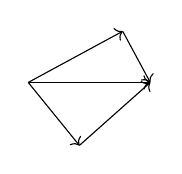
\begin{tikzpicture}
\draw[->] (0,0) -- (1.2,0.65);
\draw[->] (1.2,0.65) -- (1.55,0);
\draw[->] (0,0) -- (1.55,0);
\draw[->] (0,0) -- (0.65,-0.8);
\draw[->] (0.65,-0.8) -- (1.55,0);
\end{tikzpicture}
\end{adjustbox}
\end{center}
$\Lambda$ — граф

$\Omega$ — ориентация

$M(\Lambda,\Omega)$ —
[зачеркнуто: \Unclear{GELFAND-P001444}{category-cancelled}{пр\ldots / кат\ldots}]
категория представлений колчана

$\mathcal D(\Lambda,\Omega)$ — производная категория этой категории.

(1) \underline{Лемма.}

Тогда $\mathcal D(\Lambda,\Omega)$ не зависит от $\Omega$

($\mathcal D(\Lambda,\Omega_1)$ и $\mathcal D(\Lambda,\Omega_2)$ эквивалентны)

при разных $\Omega_1$ и $\Omega_2$

\underline{Д-во:} применение симметрии.

\underline{Задача:} найти такие
[зачеркнуто: \Unclear{GELFAND-P001444}{derived-cancelled}{$\mathcal D^{\ell}(\mathcal A)$ / $\mathcal D^{e}(\mathcal A)$ / $\mathcal D^{b}(\mathcal A)$}]
подкатегории $\mathcal A\subset\mathcal D(\Lambda,\Omega)$,
что
\begin{equation*}
\mathcal D^{\ell}(\mathcal A)=\mathcal D(\Lambda,\Omega)
\end{equation*}
\Unclear{GELFAND-P001444}{subcategory-sign}{Знак между $\mathcal A$ и $\mathcal D(\Lambda,\Omega)$ обведен: $\subset$; внутри виден угловой знак $<$ / прежняя черта.}
\Unclear{GELFAND-P001444}{derived-exponent}{Верхний индекс при $\mathcal D$: $\ell$ / $e$ / $b$.}

Все они найдены и характериз. графами Дынкина.

Используются отражения и склейки (и идеология извращенных пучков)

\underline{Замеч. ИМГ}
Классифик. вект. рассл. на $CP^n$ делается только на языке
производных категорий.

\underline{Гротендик:} тяжелым трудом добыл понятия, ведущие к производной категории
(как Микеланджело).

\underline{\underline{М.К.}}

\SourceFigure{GELFAND-P001444}{reflection-quiver}{Слева колчан с четырьмя вершинами: $V_\alpha$ слева, $V_\beta$ сверху, $V_\gamma$ справа, нижняя вершина без подписи. Стрелки идут слева к верхней, правой и нижней вершинам; от верхней и нижней — к правой. Над ребром $V_\alpha\to V_\beta$ стоит $f$; над горизонтальным ребром имеется обведенный или отмененный знак, неуверенно читаемый как $g$ / $\varphi$. Подпись этого ребра требует сверки с оригиналом.}

\underline{Отражение} а) $s_\alpha\Omega$ — обращаем стрелки,
исходящие из $\alpha$.

б)
\begin{equation*}
(s_\alpha V)_{\beta\ne\alpha}=V_\beta
\end{equation*}
\begin{equation*}
(s_\alpha V)_\alpha=\bigoplus_{\alpha\to\beta}V_\beta/(\text{образу }V_\alpha)
\end{equation*}
с соотв. отображениями

Могут быть векторы из $V_\alpha$, к-рые всюду переходят в $0$

\begin{center}
\begin{adjustbox}{max width=\linewidth}
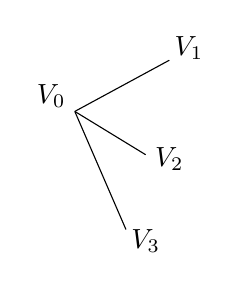
\begin{tikzpicture}
\node at (-0.3,0.2) {$V_0$};
\draw (0,0) -- (1.2,0.65);
\draw (0,0) -- (0.9,-0.55);
\draw (0,0) -- (0.65,-1.5);
\node at (1.45,0.8) {$V_1$};
\node at (1.2,-0.6) {$V_2$};
\node at (0.9,-1.65) {$V_3$};
\end{tikzpicture}
\end{adjustbox}
\end{center}
\begin{equation*}
V_0\longrightarrow V_1\oplus V_2\oplus V_3
\end{equation*}


\SourcePage{GELFAND-P001445}{30}
Построим комплекс по этим данным
\begin{equation*}
\begin{adjustbox}{max width=\linewidth}
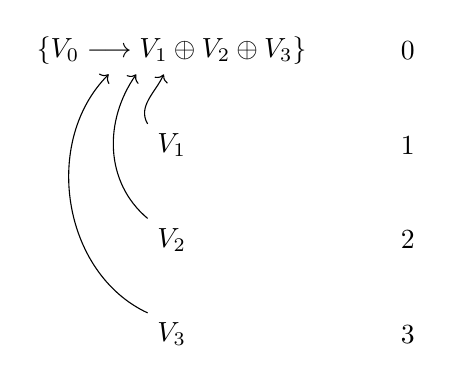
\begin{tikzpicture}
\node (c) at (0,0) {$\{V_0\longrightarrow V_1\oplus V_2\oplus V_3\}$};
\node (v1) at (0,-1.2) {$V_1$};
\node (v2) at (0,-2.4) {$V_2$};
\node (v3) at (0,-3.6) {$V_3$};
\node at (3,0) {$0$};
\node at (3,-1.2) {$1$};
\node at (3,-2.4) {$2$};
\node at (3,-3.6) {$3$};
\draw[->] (v1.north west) to[out=120,in=245] (-0.1,-0.3);
\draw[->] (v2.north west) to[out=140,in=235] (-0.45,-0.3);
\draw[->] (v3.north west) to[out=155,in=225] (-0.8,-0.3);
\end{tikzpicture}
\end{adjustbox}
\end{equation*}
Это объект производной категории (предст. колчана)
\begin{equation*}
\begin{adjustbox}{max width=\linewidth}
\begin{tikzcd}[column sep=large,row sep=small]
 & 1 \arrow[dl]\\
0 & 2 \arrow[l]\\
 & 3 \arrow[ul]
\end{tikzcd}
\end{adjustbox}
\end{equation*}
Факторизации в обычной кат. надо сопоставлять само
отображение (комплекс)

\Unclear{GELFAND-P001445}{bottom-name}{Парти… [фамилия неразборчива]} ставит и решает вопрос о том, когда производная
катег. совп. с этой (для $3^{\text{х}}$, но не для $4^{\text{х}}$).


\SourcePage{GELFAND-P001446}{unlabelled}
\underline{23. III. 88 г.}\qquad \underline{Сем. Гельфанда.}

\underline{Зелевинский А.}\qquad
\underline{Матроиды и теорема Холла}

\underline{И.М.Г.}

Матроид. [Над следующим словом зачёркнуто: \Unclear{GELFAND-P001446}{intro-deletion}{неразборчивые зачёркнутые знаки}.]
\underline{Пример:} линейно независ. системы векторов.
\begin{equation*}
M_1,M_2\text{ — мн-ва},\qquad \varphi\subset M_1\times M_2
\end{equation*}
(отношение)

Пусть на $M_1$ есть структ. матроида.

Как ввести структ. матроида на $M_2$?
\begin{equation*}
A\subset M_2,\qquad \pi_1\bigl(\pi_2^{-1}(A)\cap\varphi\bigr)
\text{ — мн-во}.
\end{equation*}
[Под тире зачёркнуто: \Unclear{GELFAND-P001446}{image-set-deletion}{неразборчиво}.]

Ранг мн-ва $A$ определяется

$1^{\circ}$. \underline{Теор. Радо}
\begin{equation*}
r_{M_2}(A)=\min_{B\subset A}
\bigl(r_{M_1}(\varphi(B))+|A-B|\bigr),\qquad A\subset M_2.
\end{equation*}

$2^{\circ}$. \underline{Теор. Холла} $\equiv$
[Над фамилией вставлено: \Unclear{GELFAND-P001446}{hall-insertion}{Ф. / $\varphi$}.]

[Зачёркнуто слева: \Unclear{GELFAND-P001446}{hall-left-deletion}{неразборчиво}.]
\underline{Зад. о выборе невест}:
[Над строкой вставлено: мн-во $M$ женихов,
$\operatorname{Card}M\geq\operatorname{Card}N$.]

Если [над $N$ вписано: мн-во] $N$ невест и
[зачёркнуто: $M\geq N$ женихов], каждому жениху $m\in M$
нравятся невесты $A(m)\subset N$; причем
[зачёркнуто: $\forall A\subset N$] $\forall$ подмн-ва
$K\subset N$,
[над формулой зачёркнуто: \Unclear{GELFAND-P001446}{card-deletion}{неразборчивый знак}.]
\begin{equation*}
\operatorname{Card}\left(\bigcup_{n\in K}B(n)\right)
\geq \operatorname{Card}K.
\end{equation*}


\SourcePage{GELFAND-P001447}{37}
(Здесь $B(n)\subset M$;
[под $B(n)$ через знак равенства:]
мн-во женихов, к-рым нравится $n$, т.е.
\begin{equation*}
B(n)=
\{m:\ n\in A(m)\}
\end{equation*}
[После $=$ зачёркнуто: \Unclear{GELFAND-P001447}{top-b-deletion}{неразборчивый знак}.])

Тогда $\exists$ вз.-однозн. выбор
[зачёркнуто: \Unclear{GELFAND-P001447}{choice-deletion}{неразборчиво}]:
отображение $f:N\longrightarrow M$, для к-рого
\begin{equation*}
f(n)\subset B(n)\qquad \forall n.
\end{equation*}
\Unclear{GELFAND-P001447}{hall-membership}{В источнике: $f(n)\subset B(n)$.}

[Зачёркнута строка: Теор. Холла\quad $\varphi$ — отношение.]

[Зачёркнуто: Теор.]
Сущ. док-во, содержащее алгоритм.

\underline{Сведение к теор. Радо}: в $N$ надо объявить все мн-ва независимыми.

$2^{\circ}\Rightarrow 3^{\circ}$. \underline{Теор. Биркгофа.}

Из теор. Холла следует, что если есть подгруппа $H\subset G$
[под $G$: кон. группа],
то $\exists$ система общих представителей левых и правых
смежных классов.

\underline{И.М.Г.} Есть неск. знаменитых задач, про к-рые всем очевидна
их бессмысленность.

\underline{Пример.} 1) \underline{Аксиома о параллельности}

(почему именно она?)

[Под этой строкой:] \Unclear{GELFAND-P001447}{parallelism-note}{занимались ими / занимались ними}

[Справа от первых двух строк, за вертикальной чертой:]
$\Rightarrow$ неевкл. геом.

2) \underline{Трисекция угла} и квадратура круга.
\begin{equation*}
\text{Трисекция угла}\ \Downarrow\ \text{теор. Галуа}
\end{equation*}

3) \underline{Теор. Ферма}
\begin{equation*}
\Downarrow
\end{equation*}
теор. [зачёркнуто: \Unclear{GELFAND-P001447}{ideals-deletion}{неразборчивая буква}] идеалов (Куммер)
и алгебр. геометрия.
[Справа, за вертикальной чертой:] раб. Фалтингса.

4) \underline{Задача о $4^{\text{х}}$ красках}
\begin{equation*}
\Downarrow\quad ?
\end{equation*}
Стоит разобрать эти работы.

5) \underline{Гипотеза Римана}


\SourcePage{GELFAND-P001448}{unlabelled}
\underline{А. Рудаков.}\quad
\underline{Векторные расслоения, группы кос и диофантовы уравнения.}

$1^{\circ}$. На $\mathbb{P}^{2}\ (= \mathbb{C}\mathbb{P}^{2})$

рассм. вект. расслоения (или ког. пучки)
\begin{equation*}
E_1,\ E_2,\ E_3 \tag{1}
\end{equation*}
[После $E_1$ зачёркнуто: \Unclear{GELFAND-P001448}{triple-deletion}{неразборчивые знаки}.]
\begin{equation*}
\begin{gathered}
\operatorname{Ext}^{k}(E_j,E_i)=0,\quad j>i,\quad k=0,1,2,\\
\operatorname{Ext}^{k}(E_i,E_i)=
\begin{cases}
0,& k>0,\\
\mathbb{C},& k=0.
\end{cases}
\end{gathered}
\tag{2}
\end{equation*}
[Перед $k=0,1,2$ зачёркнуто: \Unclear{GELFAND-P001448}{ext-deletion}{неразборчивый знак}.]

Такие существуют и если $\dim E_j=x_j$, то
\begin{equation*}
x_1^2+x_2^2+x_3^2=3x_1x_2x_3
\qquad\text{(ур-е Маркова)} \tag{3}
\end{equation*}
(и все [сверху вставлено: целочисл.] решения так реализуются!)

На наборах [сверху вставлено: (1) (их счётное мн-во)]
действ. группа кос и все наборы (1)
сост. 1 орбиту!

$2^{\circ}$.
\begin{equation*}
Q=\mathbb{P}^{1}\times\mathbb{P}^{1}.
\end{equation*}
[После $Q=$ зачёркнуто: \Unclear{GELFAND-P001448}{quadric-deletion}{неразборчивый знак}.]

Тогда берём 4 расслоения $E_1,E_2,E_3,E_4$
с теми же условиями (2); тоже действ. группа кос.

Вместо (3) возникает система диофантовых ур-й
(но соответствие в одну сторону; не доказано, что все реш. получаются).
Это что-то вроде системы корней, где вместо
гр. Вейля возникает группа кос.

$3^{\circ}$. На $\mathbb{P}^{n}$ можно рассм. расслоения
\begin{equation*}
E_1,E_2,\ldots,E_{n+1}\qquad\text{с усл. (2)}
\end{equation*}
и тоже возникает действие группы кос.

\underline{М. Капранов}: о действии группы кос.

\underline{И.М.Г.}

Разрешимые и неразрешимые классификационные задачи.

Нет парам. $\Rightarrow$ классифицируются (ручные)

1 парам $\Rightarrow$
[зачёркнуто: \Unclear{GELFAND-P001448}{classification-correction}{ручные (…)}; над строкой вставлено: полуручные] (tame)

$\geq 2$ парам. $\Rightarrow$ неразреш.
(напр., пары матриц)

и классиф. отн.
[зачёркнуто: \Unclear{GELFAND-P001448}{bottom-deletion}{неразборчиво}]
\begin{equation*}
(A,B)\mapsto(C^{-1}AC,C^{-1}BC).
\end{equation*}


\SourcePage{GELFAND-P001449}{38}
В неразреш. задачах всегда есть разрешимая часть
(открытая орбита!)

[Над инициалами зачёркнуто: \Unclear{GELFAND-P001449}{top-deletion}{Еф / неразборчиво}.]

\underline{М.К.}
\begin{equation*}
\operatorname{Ext}^{1}(E,E)=0\ \Rightarrow\ \text{жёсткость}
\end{equation*}
(и рассл. такие не имеют параметров)

[Над следующей строкой зачёркнуто: \Unclear{GELFAND-P001449}{sequence-deletion}{Пару / неразборчиво}.]
\begin{equation*}
0\longrightarrow R\longrightarrow E\otimes\operatorname{Hom}(E,F)
\longrightarrow F
\end{equation*}

Пару $(E,F)$ назовём исключительной, если
$\operatorname{Ext}^{j}(F,E)=0$.

Тогда пара $(F,R)$ тоже исключительна.

Получ. действие $\mathbb{Z}$ на таких парах;
выполняются соотношения, дающие косы.

\underline{И.М.Г.} Работа Берншт.-Гельф.-Пономарев:
в предст. графов действ. гр. Кокстера.

Что нужно для занятий, напр., спектр. теорией из общего образ.

1) Предст. графов (4-ка подпр-в и т.п.)

2) Произв. категория.

\underline{Бейлинсон А.}\qquad \underline{Извращенные пучки.}

\underline{И.М.Г.} (о Макферсоне)

\SourceFigure{GELFAND-P001449}{circle-diagram}{Круг с внутренним криволинейным треугольником и несколькими дугами между точками окружности; справа нижняя вершина и соседние дуги удвоены. Сопоставить точные соединения с оригиналом.}

Чем параметризовать эти области?
\begin{equation*}
\begin{adjustbox}{max width=\linewidth}
\begin{tikzpicture}
\draw (0,0)--(3,0);
\draw (0.6,0) circle (0.055);
\draw (1.2,0) circle (0.055);
\draw (1.85,0) circle (0.055);
\draw (2.5,0) circle (0.055);
\node[anchor=west] at (3.6,0) {4 точки на проек. прямой};
\draw (0,-0.8)--(3,-0.8);
\draw (0.6,-0.8) circle (0.055);
\draw (1.2,-0.8) circle (0.055);
\draw (1.85,-0.8) circle (0.055);
\end{tikzpicture}
\end{adjustbox}
\end{equation*}
Стратам обл. Зигеля $\Rightarrow$ конфигур. прямых на $\mathbb{R}\mathbb{P}^{2}$.

\underline{Б.}

О раб. Макферсона (о его раб. с Гельфандом и Вилоненом(?))

Извращ. пучки?

Извр. пучку соотв. задачи лин. алгебры, его полностью описывающие,
но неясно, как выделить извращ. пучки.


\SourcePage{GELFAND-P001450}{unlabelled}
$X$ — компл. мн-ие (гладкое)

\underline{Конструктивный пучок}

Задана стратификация $\{X_i\}$ [над $X_i$ с отводной чертой: откр.],
пучок $\mathcal{F}$ на $X$ наз. конструкт.
[под этим словом вписано: отн. неё],
если $\mathcal{F}|_{X_i}$ — локально пост. пучок конечномерных вкт. пр-в

(локально — отн. обычной топ.)

\underline{Конструктивные комплексы пучков}
\begin{equation*}
\ldots\longrightarrow\mathcal{F}^{-1}
\longrightarrow\mathcal{F}^{0}
\longrightarrow\mathcal{F}^{1}
\longrightarrow\mathcal{F}^{2}\longrightarrow\ldots \tag{1}
\end{equation*}
комплекс пучков наз. конструктивным, если все пучки
$H^{i}(\mathcal{F}^{\bullet})$ конструктивны.

(на $\mathcal{F}^{i}$ условий нет!)

\underline{Синг. носитель} пучка или комплекса

$\mathcal{F}^{\bullet}$ — констр. комплекс.
\begin{equation*}
SS(\mathcal{F})\subset T^{*}X \tag{2}
\end{equation*}
[Под $SS(\mathcal{F})$: подмн-ие]
определяется след. образом.

Пусть $\nu\in T_x^{*}X$, $\nu\ne0$.
\Unclear{GELFAND-P001450}{covector-letter}{Буква ковектора: $\nu$ / $v$.}

(3) \underline{Опр.}
\begin{equation*}
\nu\notin SS(\mathcal{F})\ \Longleftrightarrow
\end{equation*}
[После знака, над строкой вставлено: если]
выб. малую окр. $U\ni x$, голом. ф-ю $f$ на $U$,
для к-рой $df_x=\nu$, $f(x)=0$, то $\forall$ близкой к $0$
точки $\varepsilon\in\mathbb{C}$
\begin{equation*}
H^{*}\bigl(U,f^{-1}(\varepsilon);\mathcal{F}\bigr)=0. \tag{4}
\end{equation*}
[Под $f^{-1}(\varepsilon)$ дописано: $\cap\,U$.]

(относит. гр. когом. mod слоя)

(точнее, надо перех. к индукт. пределу)

([Зачёркнуто: \Unclear{GELFAND-P001450}{cycles-deletion}{появл. / неразборчиво}]
$\ne0\ \Longleftrightarrow$ появл. исчез. циклов)

(4) от выбора $f$ не зависит

0-е сечение?

Добавляем 0-е сечение, если $\mathcal{F}^{\bullet}$ — ненулевой комплекс.

$\mathcal{F}^{\bullet}$ — нулевой
$\Rightarrow SS(\mathcal{F}^{\bullet})\overset{\mathrm{df}}{=}\varnothing$.


\SourcePage{GELFAND-P001451}{39}
(5) \underline{Теорема.}
$SS(\mathcal{F})$ — коническое лагранжево подмн-ие

(аналитич. подмн-ие, у к-рого неособые точки лагранжевы в
обычном смысле [зачёркнут знак: \Unclear{GELFAND-P001451}{sense-correction}{закрывающая скобка / неразборчивый знак}];
равносильное условие — инволют. идеала)

Структура: объед. непривод. компонент (конечн. числа)

(6) \underline{Лемма.}
Если $Y\subset T^{*}X$ — неприв. лагранжево
конич. подмн-ие, то
\begin{equation*}
Y=N^{*}Z\qquad
\text{для нек-рого неприводимого }Z\subset X. \tag{7}
\end{equation*}
(конормальное расслоение)

(тогда $Z=\pi(Y)$, $\pi:T^{*}X\longrightarrow X$)

Здесь $N^{*}Z$ поним.
[зачёркнуто: \Unclear{GELFAND-P001451}{closure-deletion}{неразборчиво}]
как замыкание по Зарискому от
$N^{*}(\text{гл. часть }Z)$.
[После открывающей скобки зачёркнуто: \Unclear{GELFAND-P001451}{smooth-deletion}{неразборчивый знак}.]

[Зачёркнуто перед заголовком: \Unclear{GELFAND-P001451}{definition-deletion}{Извращ… / неразборчиво}.]

(8) \underline{Опред.}
Пусть зад. коническое лагр. подмн-ие $Y\subset T^{*}X$,
$f$ — голом. ф-я на $X$.

$f$ наз. морсовской отн. $Y$, если она облад. след. св-вом:

$df(X)$ (лагр. подмн-ие (не коническое!)) трансверсально $Y$,
\Unclear{GELFAND-P001451}{morse-bracket}{Перед пояснением: скобка с коротким горизонтальным штрихом.}

т.е. $df(X)$ перес. $Y$ только по гладким точкам, причем
перес. трансверсально.

\underline{Примеры.}

1. $Y=X$ — нулевое сечение.

Тогда морсовость $f$ отн. $Y$ = морсовость в обычном смысле.

2. $Y$ = конормаль к $Z$, $Y=N^{*}Z$, $Z$ — гладкое мн-ие.

Тогда морсовость означ. вып. [зачёркнуто: 2-х]
\Unclear{GELFAND-P001451}{condition-ending}{условие / условий}.

[Обозначение «а)» зачёркнуто.]
$g=f|_Z$ — морсовская ф-я (в обычн. смысле).

[Следующие две строки обведены рамкой и перечёркнуты двумя диагоналями:]
\begin{equation*}
\text{б)}\quad dg(z)=0\ \Rightarrow\ df(z)\ne0.\qquad (?)
\end{equation*}
(Если $Y$ содержит 0-е сеч., то это верно)


\SourcePage{GELFAND-P001452}{unlabelled}
(9) \underline{Опред.}
Пусть $\mathcal{F}^{\bullet}$ — конструкт. комплекс, рассм.
$SS(\mathcal{F}^{\bullet})$, $f$ — морсовская отн.
$SS(\mathcal{F}^{\bullet})$ и пусть $x$ —
критич. точка отн. $SS(\mathcal{F}^{\bullet})$
$\bigl(\overset{\mathrm{df}}{\Longleftrightarrow}
df(x)\in SS(\mathcal{F}^{\bullet})\bigr)$.
Тогда
\begin{equation*}
H^{*}\bigl(U,f^{-1}(\varepsilon);\mathcal{F}\bigr)\ne0.
\end{equation*}
Комплекс $\mathcal{F}$ наз. извращ. пучком,
если все такие группы возник. только в одной степени
(напр. 0) [зачёркнуто: \Unclear{GELFAND-P001452}{definition-deletion}{если / неразборчиво}], т.е. если
\begin{equation*}
H^{j}\bigl(U,f^{-1}(\varepsilon);\mathcal{F}\bigr)=0
\quad\text{при }j\ne0. \tag{10}
\end{equation*}
(исчез. циклы есть только в 1-й степени)
\Unclear{GELFAND-P001452}{vanishing-degree}{В источнике: «в 1-й степени».}

\underline{Примеры.}
а. $\mathbb{C}_{x_0}$ — извр. пучок.
[Под обозначением: соср. в точке.]
(слой $\mathbb{C}$ над $x_0$, $0$ на дополн.)

б. $\mathbb{C}_X[n]$ — пост. пучок над $X$
(сдвинутый по градуир.) — извращ. пучок.
\begin{equation*}
n=\dim_{\mathbb{C}}X.
\end{equation*}

в. $Z\subset X$ [с отводной чертой: гладкое подмн-ие]
\begin{equation*}
\mathbb{C}_Z[\dim Z]
\end{equation*}
[Под обозначением:]
пост. пучок на $Z$, прод. нулем вне $Z$.

(или: сдвиг комплекса Горески—Макферсона)

\underline{Замечание} (приблизительное).
Страты, отн. к-рых пучок $\mathcal{F}$ конструктивен,
суть проекции на базу неприв. компонент его $SS(\mathcal{F})$.

\underline{Конструкция 1.}
Пусть $\mathcal{F}$ — извр. пучок.
Построим лок. систему [вписано: $\Phi(\mathcal{F})$]
на гладких точках его $SS(\mathcal{F})$.

Пусть [зачёркнуто: \Unclear{GELFAND-P001452}{point-deletion}{неразборчивый знак}]
$z$ — гладкая точка $SS(\mathcal{F})$.
Тогда
\begin{equation*}
\Phi(\mathcal{F})=
H^{0}\bigl(U,f^{-1}(\varepsilon),\mathcal{F}\bigr),
\qquad df(\pi(z))=z. \tag{11}
\end{equation*}
(от выбора $f$ ничего не зависит)

\underline{След. раз — через 2 недели.}


\SourcePage{GELFAND-P001453}{unlabelled}
\Unclear{GELFAND-P001453}{page-label}{Номер листа: 42 или 48.}

\underline{11/IV--88}\quad \underline{Сем. Гельфанда}

\underline{\underline{Фукс Д.Б.}}\quad
\underline{\underline{Проблема $4^{\text{х}}$ красок.}}\quad
(Аппель; Хакен)

\underline{Опр.} Конфигурация — триангуляция диска.

[Справа зачёркнуто: «— разбиение сферы (\Unclear{GELFAND-P001453}{top-cancelled-definition}{диска?; плоск.?})
(триангуляция)».]

\SourceFigure{GELFAND-P001453}{diagram-disk}{Рисунок справа от определения: многоугольный контур с внутренними рёбрами. В нескольких местах штрихи не сходятся; точное соединение внутренних рёбер требует проверки по оригиналу.}

(1) Надо док., что вершины можно так закрасить в 4 цвета
[\Unclear{GELFAND-P001453}{line-one-cancellation}{зачёркнутый короткий фрагмент неразборчив}],
чтобы соседние вершины были раскрашены в разные цвета.

[Мелкая приписка:] (это двойств. задача к раскр. граней; поэтому
\Unclear{GELFAND-P001453}{parenthetical-tail}{другая только?; другие только?}

(2) Мн-во конфигур. наз. \underline{неизбежным}, если в каждой триангул.
одна из них встречается.

(3) Конфиг. наз. \underline{приводимой}, если она не может входить в
триангуляцию сферы, не раскрашиваемую в 4 цвета и
имеющую среди таких триангуляций наименьшее число вершин.

\underline{Привод. триангуляция $K$:}
[зачёркнуто: \Unclear{GELFAND-P001453}{reducibility-cancelled-if}{если?}; вписано сверху: «пусть»]
есть триан. $T\supset K$ и известно,
что $\forall$ конфигур. [\Unclear{GELFAND-P001453}{reducibility-cancelled-word}{зачёркнутое слово неразборчиво}]
с меньшим числом вершин (чем $T$)
раскрашивается в 4 цвета; тогда и $T$ тоже раскрашивается.

Индукция по числу вершин $N$.

\underline{Пусть для $N-1$ вершин уже доказано.}

Конфиг. [зачёркнуто: \Unclear{GELFAND-P001453}{induction-cancelled-word}{это?}] $K$ наз. \underline{приводимой}, если
[вписано сверху: «из»] её присутствия в $T$ с
$|T|=N$ следует, что $T$ раскрашивается.

[Зачёркнуто: «Пример.»]

Основная идея — соединение определений (2) и (3).

[Зачёркнуто: «Нужно»; вписано сверху: «Достаточно»]
построить неизбежный набор приводимых конфигураций.

(4) \underline{Пример.}

\begin{center}
\begin{adjustbox}{max width=\linewidth}
\begin{tikzpicture}[x=1cm,y=1cm]
\draw (0,0)--(.8,1.3)--(1.8,.1)--cycle;
\draw (.8,.55)--(0,0) (.8,.55)--(.8,1.3) (.8,.55)--(1.8,.1);
\fill (0,0) circle (2pt);
\fill (.8,1.3) circle (2pt);
\fill (1.8,.1) circle (2pt);
\fill (.8,.55) circle (2pt);
\node[anchor=west] at (2.2,.65) {— приводимая конфигурация.};
\end{tikzpicture}
\end{adjustbox}
\end{center}

\begin{center}
\begin{adjustbox}{max width=\linewidth}
\begin{tikzpicture}[x=1cm,y=1cm]
\draw (0,0)--(.8,1.3)--(1.8,.1)--cycle;
\draw (.8,.55)--(0,0) (.8,.55)--(.8,1.3) (.8,.55)--(1.8,.1);
\draw (-.65,.8)--(-.2,.4) (.4,1.9)--(.7,1.4)
      (1.6,1.8)--(1.2,1.35) (2.4,1.15)--(1.9,.55)
      (-.3,-.65)--(-.25,-.45) (.85,-.6)--(.95,-.2)
      (1.4,-.65)--(1.4,-.25) (2.25,-.5)--(2.1,-.05);
\draw[->] (2.9,.65)--(4.6,.65);
\draw (6.1,.1)--(6.9,1.2)--(7.55,.1)--cycle;
\draw (5.35,1.35)--(5.95,.55) (6.05,1.85)--(6.6,1.05)
      (7.8,1.85)--(7.55,1.2) (8.45,1.3)--(7.8,.65)
      (8.65,.3)--(7.95,-.2) (6.9,-.85)--(7.1,-.25)
      (5.85,-.9)--(6.25,-.4) (5.2,-.6)--(5.55,-.3);
\node[align=center] at (7,-1.45) {тоже\\триангуляция};
\end{tikzpicture}
\end{adjustbox}
\end{center}


\SourcePage{GELFAND-P001454}{unlabelled}
\underline{И.М.Г.} Всё надо придумывать на простейших примерах.
(И. Бернштейн этому науч. от И.М.Г.)

Теор. сферич. ф-й И.М.Г. придумал всю на ф-ле
\begin{equation*}
\cos(\alpha+\beta)+\cos(\alpha-\beta)=2\cos\alpha\cdot\cos\beta.
\end{equation*}
На $\mathbb R$ надо рассм. группу, порожденную паралл. переносами и
отражениями.

[Над следующим заголовком зачёркнуто: \Unclear{GELFAND-P001454}{cancelled-theorem-heading}{Утв.?}]

(5) \underline{Теорема}
\begin{center}
\begin{adjustbox}{max width=\linewidth}
\begin{tikzpicture}[x=1cm,y=1cm]
\draw (0,0)--(.25,1.4)--(1.7,1.45)--(1.5,.1)--cycle;
\draw (0,0)--(.88,.73)--(1.7,1.45);
\draw (.25,1.4)--(.88,.73)--(1.5,.1);
\fill (0,0) circle (2pt);
\fill (.25,1.4) circle (2pt);
\fill (1.7,1.45) circle (2pt);
\fill (1.5,.1) circle (2pt);
\fill (.88,.73) circle (2pt);
\node[anchor=west] at (2.5,.75) {приводима};
\end{tikzpicture}
\end{adjustbox}
\end{center}

(Кемпе; $\sim 100$ лет назад)

Заменим на

(6)
\begin{center}
\begin{adjustbox}{max width=\linewidth}
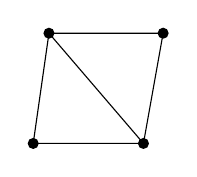
\begin{tikzpicture}[x=1cm,y=1cm]
\draw (0,0)--(.2,1.4)--(1.65,1.4)--(1.4,0)--cycle;
\draw (.2,1.4)--(1.4,0);
\fill (0,0) circle (2pt);
\fill (.2,1.4) circle (2pt);
\fill (1.65,1.4) circle (2pt);
\fill (1.4,0) circle (2pt);
\end{tikzpicture}
\end{adjustbox}
\end{center}
и раскрасим получившуюся триангуляцию.

(*) Если среди 4-х есть одинаковые, то центр раскр. в свободную.
\begin{center}
\begin{adjustbox}{max width=\linewidth}
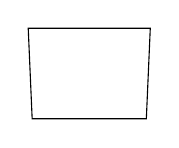
\begin{tikzpicture}[x=1cm,y=1cm]
\draw (0,0)--(-.05,1.15)--(1.5,1.15)--(1.45,0)--cycle;
\end{tikzpicture}
\end{adjustbox}
\end{center}

остаётся рассм. случай

(7)
\begin{center}
\begin{adjustbox}{max width=\linewidth}
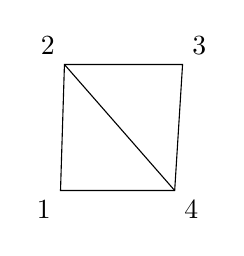
\begin{tikzpicture}[x=1cm,y=1cm]
\draw (0,0)--(.05,1.6)--(1.55,1.6)--(1.45,0)--cycle;
\draw (.05,1.6)--(1.45,0);
\node[below left] at (0,0) {$1$};
\node[above left] at (.05,1.6) {$2$};
\node[above right] at (1.55,1.6) {$3$};
\node[below right] at (1.45,0) {$4$};
\end{tikzpicture}
\end{adjustbox}
\end{center}

Рассм. подмн-во $K$, сост. из вершин, раскр. в 1 и 3
и рёбер
\begin{adjustbox}{max width=\linewidth}
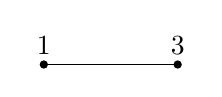
\begin{tikzpicture}[baseline=0pt,x=1cm,y=1cm]
\draw (0,0)--(1.7,0);
\fill (0,0) circle (1.5pt);
\fill (1.7,0) circle (1.5pt);
\node[above] at (0,0) {$1$};
\node[above] at (1.7,0) {$3$};
\end{tikzpicture}
\end{adjustbox}

(8) 1 может а) соединяться с 3 в $K$

или б) не соединяться.

Случай б): в этой связной компоненте вершины 1
меняем 1 и 3 местами и сводим к пред. случаю (*).

(9)
\SourceFigure{GELFAND-P001454}{diagram-path}{Квадрат с диагональю из верхней левой вершины к нижней правой; у углов подписи: слева внизу 1, слева вверху 2, справа вверху 3, справа внизу 4. Снаружи снизу и справа проходит линия со сплошной начальной частью и отдельными штрихами продолжения; у её нижних изломов видны 3, 1 и исправленная цифра, похожая на 3. Точный вид последней подписи и примыкания штрихового продолжения проверить по оригиналу.}

[Справа от рисунка:]

Пусть случай 8а).

Тогда не сущ. пути из 2 в 4
с [зачёркнуто: \Unclear{GELFAND-P001454}{cancelled-before-two}{зачёркнутый фрагмент неразборчив}] 2 и 4.

\SourceFigure{GELFAND-P001454}{diagram-excluded-edge}{Два маленьких рисунка: квадрат с диагональю и отдельно наклонное ребро. На диагонали и на отдельном ребре одинаковый петлеобразный знак исключения. Подпись справа: «— это ребро не считаем». Точный рисунок петлеобразной пометы проверить по оригиналу.}

(т.к. не может пересечь путь из 1 и 3)

и дальше опять сводим к 8б).



\SourcePage{GELFAND-P001455}{49}
% Original scan inspected directly. Reproducible review coordinates are retained in completion.json.
% Diagram (10): [100,50,645,435], 3x. Visible contour gaps and two unattached inner strokes retained.
\begin{center}
\begin{adjustbox}{max width=\linewidth}
\begin{tikzpicture}[x=0.012cm,y=-0.012cm,line width=0.5pt]
\node at (145,215) {(10)};
\draw (255,217)--(256,160)--(310,87);
\draw (345,78)--(425,72)--(510,107)--(555,160)--(550,216)--(527,270);
\draw (507,303)--(402,321);
\draw (315,278)--(280,269)--(256,231);
\draw (360,155)--(410,200);
\draw (402,250)--(472,210);
\draw (550,216)..controls (620,196) and (652,394)..(539,429)..controls (480,426) and (433,376)..(402,321);
\draw (550,216) circle (6);
\draw (402,321) circle (6);
\node at (600,186) {$1$};
\node at (390,384) {$3$};
\end{tikzpicture}
\end{adjustbox}
\end{center}
Рассм. более сложную конфигурацию
и все возможные раскраски контур.
(в 4 цвета)

Нек-рые из них продолжаются внутрь,
а нек-рые нет.

Можно пробовать перекраски как в (9) (с пол. успех).
Этим способом компьютер ищет приводимые конфигурации.

% Diagram (11): [350,660,810,1085], 4x. Nodes, unarrowed edges and embedding directly checked.
\begin{center}
\begin{adjustbox}{max width=\linewidth}
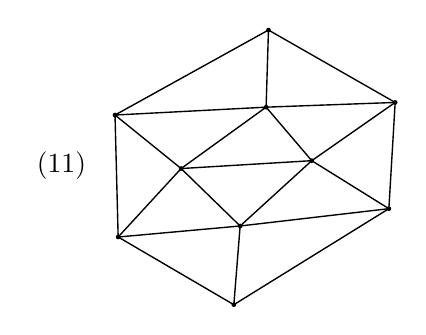
\begin{tikzpicture}[x=0.01cm,y=-0.01cm,line width=0.5pt]
\node at (335,870) {(11)};
\coordinate (a) at (598,698);
\coordinate (b) at (759,790);
\coordinate (c) at (751,925);
\coordinate (d) at (554,1047);
\coordinate (e) at (407,961);
\coordinate (f) at (403,806);
\coordinate (g) at (595,796);
\coordinate (h) at (487,874);
\coordinate (i) at (653,864);
\coordinate (j) at (562,947);
\draw (a)--(b)--(c)--(d)--(e)--(f)--(a);
\draw (a)--(g)--(b);
\draw (f)--(g)--(h)--(f);
\draw (h)--(e);
\draw (g)--(i)--(b);
\draw (h)--(i)--(c);
\draw (h)--(j)--(i);
\draw (e)--(j)--(c);
\draw (j)--(d);
\fill (a) circle (3);
\fill (b) circle (3);
\fill (c) circle (3);
\fill (d) circle (3);
\fill (e) circle (3);
\fill (f) circle (3);
\fill (g) circle (3);
\fill (h) circle (3);
\fill (i) circle (3);
\fill (j) circle (3);
\end{tikzpicture}
\end{adjustbox}
\end{center}
Приводимая конфигурация
(но Фуксу [зачёркнуто: \Unclear{GELFAND-P001455}{configuration-cancel}{у / д}] не удалось доказать)

И.М.Г. \underline{Задача} \Unclear{GELFAND-P001455}{task-number}{6 / в}.
Написать программу опред. приводимости для
параллельного компьютера.

Одна из конфигур. Аппеля и Хакена (из 1700) была проверена
вручную (Allaire), т.к. не бралась машиной.

\underline{Неизбежное мн-во.}

Их построение основано на теор. Эйлера
\begin{equation*}
\mathrm{В}-\mathrm{Р}+\mathrm{Г}=2.\tag{12}
\end{equation*}
\underline{Кемпе:} пусть \Unclear{GELFAND-P001455}{vertex-count-symbol}{$\nu_i$ / $v_i$} — число вершин, к-рые соед. ровно
с $i$ другими вершинами (из них вых. $i$ рёбер)
\begin{equation*}
\mathrm{В}=\nu_3+\nu_4+\nu_5+\ldots\tag{13}
\end{equation*}
\begin{equation*}
\mathrm{Р}=\frac{1}{2}(3\nu_3+4\nu_4+5\nu_5+\ldots)\tag{14}
\end{equation*}
% Small incident-pair sketch: original approximately [280,2500,440,2610], reviewed in equations-middle at 3x.
\begin{center}
\begin{adjustbox}{max width=\linewidth}
\begin{tikzpicture}[x=0.01cm,y=-0.01cm,line width=0.5pt]
\draw (298,2590) circle (5);
\draw (302,2585)--(430,2520);
\end{tikzpicture}
\end{adjustbox}
\end{center}
\begin{equation*}
2\mathrm{Р}=\text{число таких пар}=3\nu_3+4\nu_4+\ldots
\end{equation*}
(вершина и исх. из нее ребро)
\begin{equation*}
3\mathrm{Г}=2\mathrm{Р}\qquad\text{(т.к. триангуляция)}\tag{15}
\end{equation*}
отсюда
\begin{equation*}
\mathrm{Г}=\frac{3\nu_3+4\nu_4+5\nu_5+\ldots}{3}\tag{15'}
\end{equation*}
Из (12) находим:
\begin{equation*}
3\nu_3+2\nu_4+\nu_5-\nu_7-2\nu_8-3\nu_9-\ldots=12,\tag{16}
\end{equation*}
т.е.

[Зачёркнут номер: \Unclear{GELFAND-P001455}{cancelled-equation-number}{(17) / (16)}]
\begin{equation*}
\sum_{i=3}^{\infty}(6-i)\nu_i=12\tag{16'}
\end{equation*}

\SourcePage{GELFAND-P001456}{unlabelled}
% Original scan inspected directly. Reproducible review coordinates are retained in completion.json.
(17) Отсюда одно из чисел \Unclear{GELFAND-P001456}{vertex-count-symbol}{$\nu_3,\nu_4,\nu_5$ / $v_3,v_4,v_5$} отлично от $0$.

Получаем неизбежное мн-во

% Figure (18), first two sketches: [80,300,1680,710], 3x. The second crossing is not supplied with an invented central dot.
\begin{center}
\begin{adjustbox}{max width=\linewidth}
\begin{tikzpicture}[x=0.018cm,y=-0.018cm,line width=0.5pt]
\node at (300,390) {(18)};
\draw (377,433)--(432,328)--(484,421)--(377,433);
\draw (377,433)--(430,391)--(484,421);
\draw[line width=1pt] (432,328)--(430,391);
\fill (430,391) circle (3);
\draw (405,490)--(405,550);
\node at (435,590) {привод.};
\draw (609,372)--(667,325)--(761,355)--(657,434)--(609,372);
\draw (609,372)--(761,355);
\draw (667,325)--(657,434);
\draw (685,490)--(685,550);
\node at (685,590) {привод.};
\end{tikzpicture}
\end{adjustbox}
\end{center}
\SourceFigure{GELFAND-P001456}{diagram-18-right}{Третий рисунок в (18): пятиугольный контур с верхней вершиной, двумя боковыми и двумя нижними вершинами; внутри отмечен узел, от которого проведены пять отрезков к вершинам контура. Верхняя правая сторона обведена густым клиновидным штрихом; у её правого конца есть короткий выступ, характер которого неясен. Под рисунком вертикальный указатель к надписи «не удаётся сразу / док. приводимость».}

Теперь можно рассм. лишь триангул. с
\begin{equation*}
\nu_3=\nu_4=0\tag{19}
\end{equation*}
\underline{Discharging} (разрядка)

(20) Начальный заряд: вершине, из к-рой исх. $i$ рёбер,
припиш. заряд [зачёркнуто: \Unclear{GELFAND-P001456}{initial-charge-cancel}{$60-i$ / $6-i$}] $60(6-i)$

\underline{Процедура перезарядки:} строим другую ф-ю на вершинах.
\begin{equation*}
(16')\Longleftrightarrow\text{сумма всех зарядов}=720.
\end{equation*}
(21) Хотим [надстрочная вставка: «сделать»], чтобы все заряды были $\leq0$.

(что невозможно [зачёркнуто: \Unclear{GELFAND-P001456}{impossible-cancel}{неразборчиво}] ввиду равенства (16'))

\underline{1 процедура.}

% Figure (22): line without an arrowhead, open left endpoint and dark right endpoint; [65,1565,2210,2150], 3x.
\begin{center}
\begin{adjustbox}{max width=\linewidth}
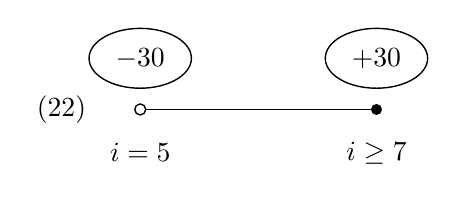
\begin{tikzpicture}[line width=0.5pt]
\node at (-1,0) {(22)};
\draw (0.07,0)--(3,0);
\draw (0,0) circle (0.07);
\fill (3,0) circle (0.07);
\draw (0,0.65) ellipse (0.65 and 0.38);
\node at (0,0.65) {$-30$};
\draw (3,0.65) ellipse (0.65 and 0.38);
\node at (3,0.65) {$+30$};
\node at (0,-0.55) {$i=5$};
\node at (3,-0.55) {$i\geq7$};
\end{tikzpicture}
\end{adjustbox}
\end{center}
(в 1-й вершине уменьшаем на 30,
во 2-й — увелич. на 30)

\underline{Неск. ситуаций, когда остается полож. заряд где-то}

(23) $1^{\circ}$.
\begin{adjustbox}{max width=\linewidth}
\begin{tikzpicture}[baseline=0pt]
\draw (0,0) circle (0.055);
\node at (0.3,0.45) {5 рёбер};
\end{tikzpicture}
\end{adjustbox}
соед. с $0$ или $1$ [зачёркнуто: \Unclear{GELFAND-P001456}{situation-one-cancel}{рёбр / рёбер}] верш. с числом рёбер $\geq7$

($\Rightarrow$ ост. вершина с полож. зарядом

[Отдельно зачёркнут знак: \Unclear{GELFAND-P001456}{cancelled-enumeration}{2 / неразборчиво}]

(24) $2^{\circ}$.
\begin{adjustbox}{max width=\linewidth}
\begin{tikzpicture}[baseline=0pt]
\fill (0,0) circle (0.055);
\node at (0,-0.5) {кр. 7};
\end{tikzpicture}
\end{adjustbox}
соед. [зачёркнуто: \Unclear{GELFAND-P001456}{situation-two-cancel}{ребра с / ребро с}] с $\leq2$ вершин кратности $5$

В итоге получ. конечный набор конфигур., к-рый неизбежен,
т.к. если нет ни одной из них, то можно сделать все
заряды $\leq0$.

\SourcePage{GELFAND-P001457}{50}
% Original scan inspected directly. Reproducible review coordinates are retained in completion.json.
Теперь надо проверить их на приводимость.

Авторы (Аппель и Хакен) в 1977 г. благодарят администр.
за 12000 часов маш. времени.
[Число 12000 волнисто подчёркнуто; под ним: «(1200?)».]

Дальше конфигур. перестраиваются в более сложные и
правила переноса тоже.

\underline{\underline{А. Бейлинсон}} (продолжение)

(о раб. К. Вилонен, С. Гельфанд, Р. Д. Макферсон)

[Под «Д.» указателем приписано: «Дункан».]

$X$ — гладкое [надстрочная вставка: «комплексное»] алгебр. мн-зие,

$\mathcal{F}$ — конечномерный констр. [зачёркнуто: «пучок»; надстрочная замена: «комплекс пучков»] на $X$.

По этим данным строится

$\mathrm{SS}(\mathcal{F})$ — лагранжево коническое мн-зие в
[зачёркнуто: $T^*X$] $\Omega X=T^*X$.

$\mathrm{SS}(\mathcal{F})=\text{нулевое сеч.}\Longleftrightarrow H^i(\mathcal{F})$ гладкий, т.е. локально постоянен

\underline{Опр.} $\mathrm{SS}\mathcal{F}$

\begin{equation*}
H^\bullet(\mathcal{F})=0\quad\Rightarrow\quad\mathrm{SS}(\mathcal{F})=\varnothing\tag{1}
\end{equation*}
\begin{equation*}
H^\bullet(\mathcal{F})\neq0\quad\Rightarrow\quad\mathrm{SS}(\mathcal{F})\supset\text{нулевое сечение},\quad\text{а}
\end{equation*}
$\mathrm{SS}(\mathcal{F})\setminus(\text{нулевое сечение})$ опис. следующим образом
\begin{equation*}
\nu\in\Omega_x^1,\qquad\text{выберем }f:\quad df_x=\nu,\quad f(x)=0
\end{equation*}
[Под $\nu$ указателем приписано: «вектор».]

Пусть $U$ — маленькая окр. точки $x$
\begin{equation*}
H^\bullet(U,U\cap f^{-1}(\varepsilon)\text{[зачёркнуто: }\mathcal{F}\text{]};\mathcal{F})
=\Phi_f^\bullet(\mathcal{F})_x\tag{2}
\end{equation*}
(пр-во исчезающих [зачёркнуто: \Unclear{GELFAND-P001457}{vanishing-cycles-cancel}{коциклов / когомол.}] циклов)

$\varepsilon\neq0$ мало

(\Unclear{GELFAND-P001457}{hypercohomology-word}{гипергомологии / гиперкогомологии})

(относит. когом. опред. через конус)
отобр., т.е. надо напис. бикомплекс и
свернуть

% Commutative square: [240,2855,2350,3410], 3x. Both upper exponents read as 1 after 10x reviews [425,3010,515,3130] and [850,3000,950,3110].
\begin{equation*}
\begin{adjustbox}{max width=\linewidth}
\begin{tikzcd}
\mathcal{F}^1(U) \arrow[r] & \mathcal{F}^1(U\cap f^{-1}(\varepsilon)) \\
\mathcal{F}^0(U) \arrow[r] \arrow[u] & \mathcal{F}^0(U\cap f^{-1}(\varepsilon)) \arrow[u]
\end{tikzcd}
\end{adjustbox}
\end{equation*}
(если $\mathcal{F}$ достаточно
ацикличен)

\SourcePage{GELFAND-P001458}{unlabelled}
% Original scan inspected directly. Reproducible review coordinates are retained in completion.json.
объяснение того, [зачёркнуто: \Unclear{GELFAND-P001458}{top-cancellation}{почему / зачем}; над строкой вставлено: при чём] здесь исчезающие циклы.

\SourceFigure{GELFAND-P001458}{vanishing-cycle-sketch}{Вверху слева несколько дуг сходятся в одну точку; справа узкий заштрихованный овал между двумя дугами. Ниже горизонтальный овал с двумя точками и соединяющим их штрихом с головкой у левой точки. От верхнего правого овала к правой нижней точке идёт прерывистая линия. Точная геометрия и направление отдельных штрихов требуют сверки с оригиналом.}

[Справа от рисунка:] цикл \Unclear{GELFAND-P001458}{cycle-caption}{стян. / стяг.} в точку

\underline{Df.} $\nu\notin SS(\mathcal F)\Longleftrightarrow$ исчез. циклы в $\nu$ равны $0$, т.е. \Unclear{GELFAND-P001458}{vanishing-cycles-degree}{$\Phi_f^i(\mathcal F)_x=0$ / $\Phi_f^\bullet(\mathcal F)_x=0$ / $\Phi_f^*(\mathcal F)_x=0$}.

Рассм. прямой образ $\mathcal F|_U$ при отобр. $U\overset{f}{\longrightarrow}\text{диск}$.

Исчез. циклы меряют, насколько слой в т. $0$ отличается от соседних слоёв.

$f$ наз. \underline{морсовской} ф-ей на $X$, если [над строкой вставлено: $f$ голоморфная ф-я на $X$ и] график $df(X)\subset$ [зачёркнуто: \Unclear{GELFAND-P001458}{cotangent-cancellation}{неразборчивый знак}] $\Omega^1$ трансверсально пересекает $SS(\mathcal F)$.

Комплекс наз. \underline{извращ. пучком}, если $\forall$ морсовской отн. $\mathcal F$ ф-и имеются исчез. циклы лишь в размерности $0$.

(только $\Phi_f^0(\mathcal F)\neq0$)

$\mathcal F$ — извращ. пучок.

По нему строится \underline{лок. система на рег. точках син. носителя}.

Её слой над точкой $\nu$:
\begin{equation*}
\Phi(\mathcal F)_\nu=\Phi_f^0(\mathcal F)_x
\end{equation*}
для морсовской ф-и $f$ с $df(x)=\nu$, \Unclear{GELFAND-P001458}{normalization-argument}{$f(0)=0$}.

Что происходит в особых точках?

\underline{Задача}: описать извр. пучки микролокальным способом,
т.е. в терминах исчез. циклов.

Она решена в работе наполовину.

\underline{Смысл}: откуда берутся извращ. пучки?

$1^\circ$. $\mathcal M$ — переопр. система

[Под словом «система»:] (голон.)

[Справа:] $\sum f_i\partial^i$

[Под $f_i$ вертикальная черта к подписи:] голом.

\begin{equation*}
\mathcal F^{0,0}\overset{\bar\partial}{\longrightarrow}\mathcal F^{0,1}\longrightarrow\cdots
\end{equation*}

[Над началом следующей строки отдельный знак:] \Unclear{GELFAND-P001458}{lower-detached-mark}{4 / знак вставки}

если $u\in\mathcal F^{0,0}$ — решение $\mathcal M$, то $\bar\partial u$ тоже

Система переопред, $\Rightarrow$ комплекс решений — извращ. пучок.

\SourcePage{GELFAND-P001459}{51}
% Original scan inspected directly. Reproducible review coordinates are retained in completion.json.
$2^\circ$. Комбинаторный способ

(Горески — Макферсон)

Есть [вставлено над строкой: общий] способ продолжения пучков в особ. точки $\Rightarrow$ получаются [зачёркнуто: \Unclear{GELFAND-P001459}{upper-cancellation}{неразборчивое слово}] извращ. пучки.

Работа посвящена $3$-му способу.

\underline{След. раз} $(18/\mathrm{IV})$ докл. \underline{Решетихина} о квант. группах.

[Ниже горизонтальная черта. Под ней у нижнего края текстового фрагмента: \Unclear{GELFAND-P001459}{bottom-cutoff}{обрезанные штрихи, возможно «М...»}.]

\SourcePage{GELFAND-P001460}{unlabelled}
% Original scan inspected directly. Reproducible review coordinates are retained in completion.json.
\underline{18.4.1988 г.}\qquad \underline{\underline{Сем. Гельфанда.}}

% The following heading has a wavy underline in the source. The author names in the left margin have broken underlines.
\underline{Назв. докладов сем. Бурбаки} $(87-88\text{ г.})$

\underline{Лернер.}\quad "Принцип неопр. и микролокализация" (по Феферману и Фонгу)

"Геом. полиномов и метод Ньютона" (по Смейлу и Шубу)

"Смешанные нелин. задачи"

"Некоммут. стох. исчисление"

"Метаплектич. предст. и гипотеза Хау"

"Пробл. Шоттки и гип. Новикова"

\underline{Дуади.}\quad "Диски Зигеля и кольцо Хермана"

"Деформации плоских кривых"

"Большие уклонения"

"Классиф. унитарных предст. вещ. групп"

"Теория классификации"

"Стаб. пучки и [зачёркнуто: \Unclear{GELFAND-P001460}{stable-cancellation}{неразборчивое слово}]
% No clear closing quotation mark survives after the cancelled material.

"Moonshine"

\underline{Вердье.}\quad "Квант. группы\Unclear{GELFAND-P001460}{quantum-title-mark}{[надстрочный знак: зачёркнутые кавычки / звёздочка]} (по Дринфельду)"

\underline{Мальгранж.}\quad "Геометрич. преобр. Фурье"

"Новые инварианты гомологич. сфер разм. $3$"

"Эллиптич. когомологии"

"Посл. достижения в теор. Ферма".

\SourcePage{GELFAND-P001461}{63}
% Original scan inspected directly. Reproducible review coordinates are retained in completion.json.
% Source has a straight underline under the surname and a wavy underline under «о раб. Атьи».
\underline{Бейлинсон} \underline{о раб. Атьи} и кого-то ещё.

\underline{Полубесконечная теория Морса.}

В $\infty$-мерном случае есть 2 вар. теории Морса (для вычисл. гомологий).

1) Зад. о геодезич. с ф-лом энергии похожа на конечномерную.
Отриц. индекс инерции конечен и равен числу сопр. точек на геодезической.

2) $\infty$-мерн. мн-зие, ф-л типа энергии
с изолир. критич. точками, но с $\infty$ числом $+$ и $\infty$ числом $-$.
Но оказ., что у двух разных крит. точек число $-$ отлич. на конечное
число; строятся гомологии, отсчит. от $\infty/2$
(топ. вариант Фейгина и Цыгана)

% «Сенсация» is wavy-underlined in the source.
\underline{Сенсация}: эти инвар. связаны с инвариантами Дональдсона
4-мерных мн-зий.

% Diagram at source (250,1285,910,1515): vertical oval, wider partly dashed outline, right arrow to M.
\begin{center}
\begin{adjustbox}{max width=\linewidth}
\begin{tikzpicture}[x=1cm,y=1cm]
\draw (0,0) ellipse (0.30 and 0.43);
\draw (-0.30,0.44) .. controls (-0.18,0.47) and (-0.08,0.44) .. (0.01,0.44);
\draw (0.02,0.49) .. controls (0.39,0.66) and (0.67,0.30) .. (0.48,-0.04);
\draw (-0.76,0.17) .. controls (-0.88,0.11) and (-0.85,0.00) .. (-0.84,-0.11);
\draw (-0.82,-0.33) .. controls (-0.72,-0.39) and (-0.62,-0.43) .. (-0.55,-0.45);
\draw (-0.34,-0.51) .. controls (-0.20,-0.50) and (-0.13,-0.58) .. (-0.04,-0.53);
\draw (0.19,-0.46) -- (0.39,-0.35);
\draw[->] (0.98,0.02) -- (2.38,0.02);
\node at (2.84,0.02) {$M$};
\node at (0.40,-0.91) {$S^1\subset\mathbb C P^1$};
\node at (2.93,-0.91) {(напр. $\mathbb C$)};
\end{tikzpicture}
\end{adjustbox}
\end{center}

Выделим для $S^1\to\mathbb C$ 2 половинки (продолж. внутрь и наружу);
они пересек. по конечномерному мн-зию.

\SourceFigure{GELFAND-P001461}{surface-sketch}{Слева овальный контур с двумя маленькими петлеобразными штрихами внутри; снаружи более широкий, частично пунктирный контур. Точное соединение верхнего внутреннего штриха с контуром и смысл внутренних петель требуют сверки с оригиналом.}
[Под рисунком:] рим. пов. $\subset$ сфера

[Справа от рисунка:] калибр. поля; ф-л Я.-М.
крит. точки — плоские связности.

\underline{И.М.Г.} Разлож. $C^\infty(S^1)$ эксплуатировалось нами ($\sim20$ лет)
(в т.ч. $\tau$-ф-и Хирота-Сато, $\frac12$-когомологии)

Замечательно, что можно заменить $S^1$ другими мн-зиями.
Это будет в след. раз.

\underline{\underline{Решетихин}} \underline{Коля}.

[Зачёркнуто и подчёркнуто: Квантовые группы.]

$\underline{U_q(SU(2))}$ \underline{и инварианты зацеплений и предст. группы кос.}

\begin{equation*}
A=\underset{\text{ассоц. алг.}}{U_q(SU(2))};\qquad
1,H,X^\pm\quad\text{— образующие}
\end{equation*}
\begin{equation*}
[X^\pm,H]=\mp2X^\pm;
\tag{1}
\end{equation*}
\begin{equation*}
[X^+,X^-]=\frac{\operatorname{sh}\left(\frac h2 H\right)}{\operatorname{sh}(h/2)};
\qquad q=e^h
\end{equation*}

\SourcePage{GELFAND-P001462}{unlabelled}
% Original scan inspected directly. Reproducible review coordinates are retained in completion.json.
% Basis monomial is wavy-underlined in source; denominator of the exponent is 4 (7x review).
\begin{equation*}
\underline{\left(q^{H/4}\right)^\ell H^n(X^+)^m(X^-)^k}
\quad\text{— базис как лин. пр-ва}
\tag{2}
\end{equation*}

\begin{equation*}
\Delta:A\to A\otimes A
\end{equation*}
\begin{equation*}
\Delta(H)=H\otimes1+1\otimes H
\tag{3}
\end{equation*}
\begin{equation*}
\Delta(X^\pm)=X^\pm\otimes q^{H/4}+q^{-H/4}\otimes X^\pm
\end{equation*}

1. $\Delta$ — гом. алгебр. $\Delta(ab)=\Delta(a)\Delta(b)$

2. $\Delta$ — коассоц., т.е.
\begin{center}
\begin{adjustbox}{max width=\linewidth}
\begin{tikzcd}[column sep=large,row sep=large]
& A\otimes A \arrow[dr,"\mathrm{id}\otimes\Delta"] & \\
A \arrow[ur,"\Delta"] \arrow[dr,"\Delta"'] & & A\otimes A\otimes A \\
& A\otimes A \arrow[ur,"\Delta\otimes\mathrm{id}"'] &
\end{tikzcd}
\end{adjustbox}
\end{center}
[Справа:] (ал. Хопфа)

3. [Зачёркнуто: \Unclear{GELFAND-P001462}{antipode-cancelled-sign}{неразборчивый знак}.]
$S:A\to A$ антигомоморфизм (аналог перех. к обр.
элементу в алгебре ф-й на группе)

\begin{equation*}
S(X^\pm)=q^{H/2}X^\pm q^{-H/2}
\tag{4}
\end{equation*}
\Unclear{GELFAND-P001462}{antipode-formula}{[Формула (4): так в источнике.]}
\begin{equation*}
S(H)=-H
\end{equation*}
\begin{equation*}
\epsilon(H)=\epsilon(X^\pm)=0
\end{equation*}

\begin{center}
\begin{adjustbox}{max width=\linewidth}
\begin{tikzcd}[column sep=large,row sep=large]
& A\otimes A \arrow[r,shift left=1.2ex,"S\otimes\mathrm{id}"] \arrow[r,shift right=1.2ex,"\mathrm{id}\otimes S"'] & A\otimes A \arrow[dr,"m"] & \\
A \arrow[ur,"\Delta"] \arrow[drr,"\epsilon"'] & & & A \\
& & \mathbb C \arrow[ur,"e"'] &
\end{tikzcd}
\end{adjustbox}
\end{center}
[Справа:] (можно брать любую из стрелок)

Превр. в квадр. алгебру в [Вставлено над строкой: других] образующих
[Зачёркнуто: \Unclear{GELFAND-P001462}{cancelled-generators}{возможно, $K,X^\pm$, затем неразборчивые штрихи}.]

Рассм.
\begin{equation*}
K=q^{H/2},\qquad K,X^\pm
\end{equation*}
[Слева зачёркнуто: $K,X^\pm$.]
\begin{equation*}
KX^\pm=q^{\pm1}X^\pm K
\end{equation*}
\begin{equation*}
X^+X^- -X^-X^+=\frac{K-K^{-1}}{q-q^{-1}}
\end{equation*}
\Unclear{GELFAND-P001462}{commutator-normalization}{[Знаменатель $q-q^{-1}$: так в источнике.]}

\SourcePage{GELFAND-P001463}{64}

(5) инволюция
\begin{equation*}
(X^+)^*=X^-,\qquad H^*=H
\end{equation*}

конечномерные предст.
\begin{equation*}
\pi_j(X^{\pm})e_m^j=
\sqrt{\frac{\operatorname{sh}\bigl(\frac h2(j\mp m)\bigr)
\operatorname{sh}\bigl(\frac h2(j\pm m+1)\bigr)}
{\operatorname{sh}^{2}\bigl(\frac h2\bigr)}}\,e_{m\pm1},
\qquad j\in\mathbb Z/2,
\qquad -j\le m\le j
\tag{6}
\end{equation*}
\begin{equation*}
\dim V^j=2j+1\quad\text{(как для $\mathrm{SL}_2$)}
\end{equation*}

Склянин писал в квадр. алгебрах.

\underline{Упражн.} \underline{(И. М. Г.)} $q=1\ \Rightarrow$ ф-лы из кн. Гельф.-Минлос-Шапиро

[Справа, выделено скобкой:] \underline{конкр. зад.}: как разл. вект. поля на сфере по сферич. \Unclear{GELFAND-P001463}{exercise-harmonics}{гар-ям / гар-м}

начать с $\mathrm{SU}(2)$

(7) \underline{Теор.} Положим
\begin{equation*}
R=\exp\left(\frac h4 H\otimes H\right)
\sum_{n\ge0}\frac{q^n}{[n]_q!}\,e^n\otimes f^n
\tag{8}
\end{equation*}
\Unclear{GELFAND-P001463}{r-coefficient}{Коэффициент в (8): $q^n/[n]_q!$ [так в записи].}
\begin{equation*}
R\in U_q(\mathrm{SU}(2))^{\otimes2},
\end{equation*}
где
\begin{equation*}
e=q^{H/4}X^+,\qquad f=q^{-H/4}X^-,
\tag{9}
\end{equation*}

(10) 1.
\begin{equation*}
(\Delta\otimes\mathrm{id})R=R_{23}R_{13},
\qquad (\in U_q(\mathrm{SU}(2))^{\otimes3})
\end{equation*}
[Перед скобкой справа зачёркнуто: \Unclear{GELFAND-P001463}{cancelled-before-membership}{неразборчиво}.]
\begin{equation*}
(\mathrm{id}\otimes\Delta)R=R_{12}R_{13};
\end{equation*}
\begin{equation*}
2.\quad \sigma\circ\Delta(a)=R\,\Delta(a)R^{-1};\qquad\text{(см. (12))}
\end{equation*}
\begin{equation*}
3.\quad R_{12}R_{13}R_{23}=R_{23}R_{13}R_{12}.
\end{equation*}
[Справа:] (ур-е Янга-Бакстера со знач. в тенз. произв. 3-х экз. $A$)

В ф-ле (8)
\begin{equation*}
[n]_q!=[n]_q\ldots[1]_q\qquad\text{($q$-факториал)}
\tag{11}
\end{equation*}

\underline{И. М. Г.} Квантовая мех. — правильный способ вводить $q$.

\underline{\underline{Упр.}} что такое $\Gamma_q$?

\begin{equation*}
\sigma\colon A^{\otimes2}\longrightarrow A^{\otimes2},\qquad
\sigma(f\otimes g)=g\otimes f
\tag{12}
\end{equation*}
В частности, из $(10)_2$ следует, что $\sigma\circ\Delta$ — тоже коумножение.

\SourcePage{GELFAND-P001464}{unlabelled}

Определим
\begin{equation*}
R^{j_1j_2}\colon V^{j_1}\otimes V^{j_2}\longrightarrow V^{j_2}\otimes V^{j_1}
\end{equation*}
\Unclear{GELFAND-P001464}{definition-separator}{После $R^{j_1j_2}$ исправленный знак: $:$; первоначальные штрихи неразборчивы.}

$V^j$ — пр-во конечномерн. предст.

\begin{equation*}
R^{j_1j_2}=P^{j_1j_2}\,\pi^{j_1}\otimes\pi^{j_2}(R)
\tag{13}
\end{equation*}
[Под $P^{j_1j_2}$, соединено чертой:] опер. перестановки пр-в

\begin{equation*}
\begin{aligned}
&(1\otimes R^{j_1j_2})(R^{j_1j_3}\otimes1)(1\otimes R^{j_2j_3})=\\
&\qquad=(R^{j_2j_3}\otimes1)(1\otimes R^{j_1j_3})(R^{j_1j_2}\otimes1)
\end{aligned}
\tag{14}
\end{equation*}

$q$-аналоги [зачёркнуто: \Unclear{GELFAND-P001464}{cancelled-coefficient}{неразборчивый знак}] коэфф. Клебша-Гордана.

все конечномерн. предст. вполне прив.

\begin{equation*}
V^{j_1}\otimes V^{j_2}=\sum_{|j_1-j_2|\le j_3\le j_1+j_2}^{\oplus}V^{j_3}
\tag{15}
\end{equation*}
\Unclear{GELFAND-P001464}{sum-mark}{Знак над суммой: $\oplus$; возможно, исправление $\otimes$ на $\oplus$.}

$V_j$ нашли Кулиш и Решетихин (1981)

В базисе:
\begin{equation*}
e_{m_1}^{j_1}\otimes e_{m_2}^{j_2}=
\sum_{|j_1-j_2|\le j_3\le j_1+j_2}
\begin{bmatrix}
j_1&j_2&j_3\\
m_1&m_2&m_3
\end{bmatrix}e_{m_3}^{j_3}
\tag{16}
\end{equation*}
[От квадратной скобки проведена черта к подписи:] коэфф. Клебша-Гордана

где
\begin{equation*}
m_3=m_1+m_2
\end{equation*}

Графич. запись:
\begin{equation*}
A\colon V^{j_1}\otimes\ldots\otimes V^{j_N}
\longrightarrow V^{j'_1}\otimes\ldots\otimes V^{j'_L}
\end{equation*}

(17)
\begin{center}
\begin{adjustbox}{max width=\linewidth}
\begin{tikzpicture}[x=1cm,y=1cm]
\draw (0,0.08)--(0,1.65)--(3.25,1.65)--(3.25,0)--(0,0);
\node at (1.63,0.82) {$A$};
\draw (0.35,1.65)--(0.35,2.55);
\draw (1.25,1.65)--(1.25,2.55);
\draw (3.1,1.65)--(3.1,2.55);
\node[left] at (0.25,2.28) {$j'_1$};
\node[left] at (1.15,2.28) {$j'_2$};
\node at (2.2,2.15) {$\ldots$};
\node[right] at (3.1,2.28) {$j'_L$};
\draw (0.4,0)--(0.4,-1);
\draw (1.35,0)--(1.35,-1);
\draw (2.97,0)--(2.97,-0.87);
\node[below] at (0.13,-1.04) {$j_1$};
\node[below] at (1.17,-1.04) {$j_2$};
\node[below] at (3.15,-1.04) {$j_N$};
\end{tikzpicture}
\end{adjustbox}
\end{center}

\begin{equation*}
A^{m'_1\ldots m'_N}_{m_1\ldots m_L}
\end{equation*}
\Unclear{GELFAND-P001464}{coefficient-range}{Индексы коэффициента: сверху $m'_1\ldots m'_N$, снизу $m_1\ldots m_L$ [так в записи].}
\begin{equation*}
-j_i\le m_i\le j_i;
\end{equation*}

[Справа внизу:]
\SourceFigure{GELFAND-P001464}{diagram-02}{Прямоугольник с $A$ и тремя вертикальными выводами сверху и снизу, без стрелок. У верхних выводов: $j'_1$, $j'_2$, $j'_L$; над ними: $m'_1$, $m'_2$, многоточие, $m'$ с исправленным последним индексом ($L$ или $N$). У нижних выводов: $j_1$, $j_2$, $j_N$; ниже: $m_1$, $m_2$, $m_N$. Требует проверки исходный знак под исправленным верхним правым индексом.}


\SourcePage{GELFAND-P001465}{65}
Произведение $BA$ изображ. соединением:

(18) \SourceFigure{GELFAND-P001465}{eq18-composition}{Слева прямоугольник с надписью $BA$, с тремя нитями сверху и тремя снизу. Над верхними концами стоят $m'_1,m'_2,m'_M$; у верхних нитей — $j'_1,j'_2,j'_M$; у нижних — $j_1,j_2,j_L$, ниже — $m_1,m_2,m_L$. После знака равенства два прямоугольника, $B$ над $A$, соединённые тремя нитями. У верхних нитей $B$ видны $j''_1,j''_2$ и $j_M$ с неуверенно читаемым штрихом; над правой нитью — $m'_M$. Первые два верхних конца подходят к строке заголовка. На соединяющих нитях — $j'_1,j'_2,j'_L$. У нижних нитей $A$ — $j_1,j_2$ и знак, похожий на $j_M$; ниже — $m_1,m_2,m_L$. Далее равенство, сумма с подписью $m'_1\ldots m'_L$ и два раздельных, не подписанных внутри прямоугольника один над другим. У каждого по три конца сверху и снизу; между прямоугольниками подписи $m'_1,m'_2,m'_L$. Число штрихов при части $j$ и последний нижний индекс у $A$ требуют сверки с оригиналом.}

\begin{equation*}
V^j\overset{id}{\longrightarrow}V^j
\quad\text{изображ. ниткой}\quad
\begin{adjustbox}{max width=\linewidth}
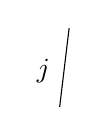
\begin{tikzpicture}[baseline=(current bounding box.center),x=1cm,y=1cm]
\draw (0,0)--(0.12,1);
\node[left] at (0,0.45) {$j$};
\end{tikzpicture}
\end{adjustbox}
\tag{19}
\end{equation*}

(20) \SourceFigure{GELFAND-P001465}{eq20-crossing}{Две пересекающиеся нити. Сверху слева $j_2$, сверху справа $j_1$; снизу слева $j_1$, снизу справа $j_2$. Нить от верхнего левого к нижнему правому концу непрерывна; другая прервана у пересечения. У нижнего правого конца есть утолщённый острый штрих, направление стрелки по нему не установлено.}
\Unclear{GELFAND-P001465}{eq20-v-indices}{$R^{j_1j_2}:V^{j_1}\otimes V^{j_1}\longrightarrow V^{j_1}\otimes V^{j_1}$}

\begin{equation*}
\begin{adjustbox}{max width=\linewidth}
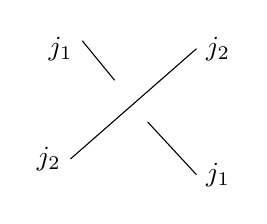
\begin{tikzpicture}[baseline=(current bounding box.center),x=1cm,y=1cm]
\draw (-0.8,-0.7)--(0.8,0.7);
\draw (-0.65,0.8)--(-0.24,0.30);
\draw (0.18,-0.23)--(0.8,-0.9);
\node[left] at (-0.65,0.7) {$j_1$};
\node[right] at (0.8,0.7) {$j_2$};
\node[left] at (-0.8,-0.7) {$j_2$};
\node[right] at (0.8,-0.9) {$j_1$};
\end{tikzpicture}
\end{adjustbox}
\qquad (R^{j_2j_1})^{-1}\qquad\text{в том же пр-ве.}
\tag{20'}
\end{equation*}

\begin{equation*}
RR^{-1}=I\qquad
\begin{adjustbox}{max width=\linewidth}
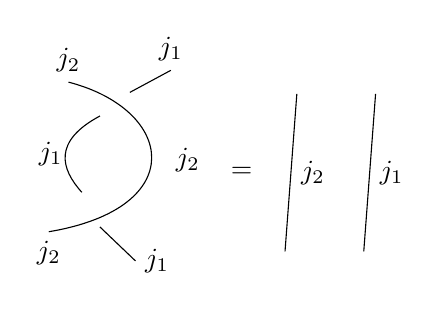
\begin{tikzpicture}[baseline=(current bounding box.center),x=1cm,y=1cm]
\draw (-0.55,1.15).. controls (0.8,0.8) and (1.0,-0.45)..(-0.8,-0.75);
\draw (0.75,1.3)--(0.23,1.02);
\draw (-0.15,0.72).. controls (-0.75,0.4) and (-0.65,0.05)..(-0.38,-0.25);
\draw (-0.15,-0.69)--(0.30,-1.12);
\node[above] at (-0.55,1.15) {$j_2$};
\node[above] at (0.75,1.3) {$j_1$};
\node[left] at (-0.50,0.24) {$j_1$};
\node[right] at (0.69,0.16) {$j_2$};
\node[below] at (-0.8,-0.75) {$j_2$};
\node[right] at (0.30,-1.12) {$j_1$};
\node at (1.65,0) {$=$};
\draw (2.2,-1)--(2.35,1);
\draw (3.2,-1)--(3.35,1);
\node[right] at (2.28,0) {$j_2$};
\node[right] at (3.28,0) {$j_1$};
\end{tikzpicture}
\end{adjustbox}
\end{equation*}

$j_1,j_2$ — цвета ниток

% В источнике заголовок подчёркнут волнистой линией.
\underline{Соотн. Янга-Бакстера}

\begin{equation*}
\begin{adjustbox}{max width=\linewidth}
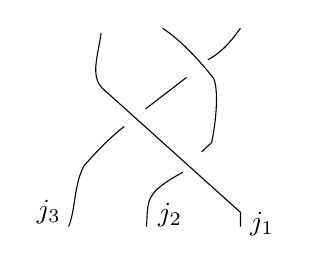
\begin{tikzpicture}[baseline=(current bounding box.center),x=0.006cm,y=-0.006cm]
\draw (70,10).. controls (62,65) and (45,106)..(78,132)
 --(365,390)--(365,420);
\draw (200,0).. controls (243,28) and (286,78)..(308,106)
 .. controls (319,130) and (314,195)..(304,242)--(283,262);
\draw (243,305).. controls (160,350) and (170,365)..(166,420);
\draw (1,420).. controls (16,385) and (12,330)..(34,291)
 .. controls (64,257) and (86,234)..(119,208);
\draw (164,171)--(251,104);
\draw (296,67).. controls (333,46) and (350,20)..(365,0);
\node[left] at (5,389) {$j_3$};
\node[right] at (170,396) {$j_2$};
\node[right] at (365,414) {$j_1$};
\end{tikzpicture}
\end{adjustbox}
\quad =\quad
\begin{adjustbox}{max width=\linewidth}
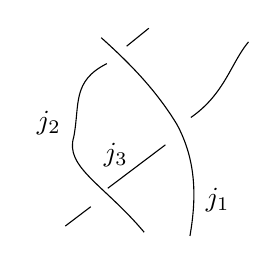
\begin{tikzpicture}[baseline=(current bounding box.center),x=0.006cm,y=-0.006cm]
\draw (90,20).. controls (164,86) and (212,141)..(250,203)
 .. controls (292,280) and (292,360)..(278,440);
\draw (191,0)--(144,38);
\draw (102,75).. controls (28,112) and (45,161)..(32,230)
 .. controls (12,294) and (96,331)..(181,432);
\draw (14,419)--(68,378);
\draw (104,339)--(226,247);
\draw (280,189).. controls (352,139) and (365,73)..(402,29);
\node[left] at (25,200) {$j_2$};
\node at (121,268) {$j_3$};
\node[right] at (291,364) {$j_1$};
\end{tikzpicture}
\end{adjustbox}
\tag{21}
\end{equation*}

Доп. вершины

\begin{equation*}
\begin{adjustbox}{max width=\linewidth}
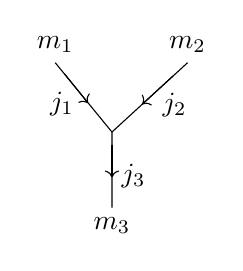
\begin{tikzpicture}[baseline=(current bounding box.center),x=0.8cm,y=0.8cm]
\draw (-0.9,1.1)--(0,0)--(0,-1.2);
\draw (1.2,1.1)--(0,0);
\draw[->] (-0.75,0.92)--(-0.38,0.46);
\draw[->] (0.97,0.89)--(0.48,0.44);
\draw[->] (0,-0.2)--(0,-0.72);
\node[above] at (-0.9,1.1) {$m_1$};
\node[above] at (1.2,1.1) {$m_2$};
\node[left] at (-0.45,0.45) {$j_1$};
\node[right] at (0.65,0.43) {$j_2$};
\node[right] at (0,-0.7) {$j_3$};
\node[below] at (0,-1.2) {$m_3$};
\end{tikzpicture}
\end{adjustbox}
\overset{\text{изобр.}}{\longrightarrow}
\begin{bmatrix}j_1&j_2&j_3\\m_1&m_2&m_3\end{bmatrix}_q
\overset{\text{или}}{\longleftarrow}
\begin{adjustbox}{max width=\linewidth}
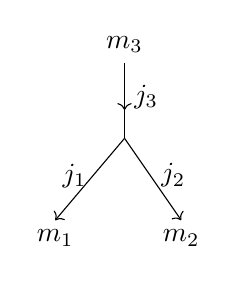
\begin{tikzpicture}[baseline=(current bounding box.center),x=0.8cm,y=0.8cm]
\draw (0,1.2)--(0,0);
\draw[->] (0,0.95)--(0,0.45);
\draw[->] (0,0)--(-1.1,-1.3);
\draw[->] (0,0)--(0.9,-1.3);
\node[above] at (0,1.2) {$m_3$};
\node[right] at (0,0.65) {$j_3$};
\node[left] at (-0.45,-0.60) {$j_1$};
\node[right] at (0.43,-0.59) {$j_2$};
\node[below] at (-1.1,-1.3) {$m_1$};
\node[below] at (0.9,-1.3) {$m_2$};
\end{tikzpicture}
\end{adjustbox}
\tag{22}
\end{equation*}

\SourcePage{GELFAND-P001466}{unlabelled}
\begin{equation*}
\begin{adjustbox}{max width=\linewidth}
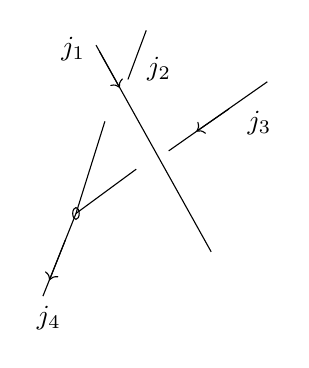
\begin{tikzpicture}[baseline=(current bounding box.center),x=0.75cm,y=0.75cm]
\draw (-0.5,2.6)--(1.45,-0.9);
\draw[->] (-0.44,2.49)--(-0.10,1.88);
\draw (0.35,2.85)--(0.04,2.02);
\draw (-0.35,1.31)--(-0.84,-0.25)--(-1.4,-1.65);
\draw[->] (-1.02,-0.70)--(-1.29,-1.38);
\draw (2.40,1.98)--(0.73,0.81);
\draw[->] (1.75,1.52)--(1.20,1.14);
\draw (0.18,0.50)--(-0.84,-0.25);
\draw (-0.84,-0.25) ellipse (0.055 and 0.10);
\node[left] at (-0.52,2.54) {$j_1$};
\node[right] at (0.20,2.20) {$j_2$};
\node[right] at (1.90,1.28) {$j_3$};
\node[below] at (-1.30,-1.66) {$j_4$};
\end{tikzpicture}
\end{adjustbox}
\quad =\quad
\begin{adjustbox}{max width=\linewidth}
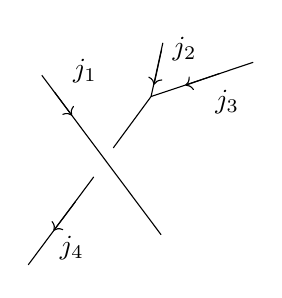
\begin{tikzpicture}[baseline=(current bounding box.center),x=0.75cm,y=0.75cm]
\draw (-1.4,1.8)--(0.62,-0.9);
\draw[->] (-1.18,1.51)--(-0.89,1.12);
\draw (0.65,2.35)--(0.45,1.44);
\draw[->] (0.63,2.24)--(0.50,1.64);
\draw (2.18,2.02)--(0.45,1.44)--(-0.19,0.57);
\draw[->] (1.61,1.83)--(1.03,1.63);
\draw (-0.52,0.08)--(-1.63,-1.41);
\draw[->] (-0.83,-0.34)--(-1.20,-0.83);
\node[above] at (-0.67,1.50) {$j_1$};
\node[right] at (0.65,2.25) {$j_2$};
\node[below] at (1.74,1.71) {$j_3$};
\node[right] at (-1.26,-1.13) {$j_4$};
\end{tikzpicture}
\end{adjustbox}
\tag{23}
\end{equation*}

\begin{equation*}
\begin{adjustbox}{max width=\linewidth}
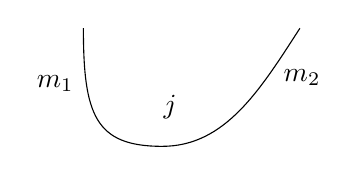
\begin{tikzpicture}[baseline=(current bounding box.center),x=1cm,y=1cm]
\draw (-1.2,0.8).. controls (-1.2,-0.3) and (-1.05,-0.7)..(-0.2,-0.7)
 .. controls (0.6,-0.7) and (1.04,0.01)..(1.55,0.8);
\node[left] at (-1.2,0.1) {$m_1$};
\node[right] at (1.22,0.17) {$m_2$};
\node at (-0.10,-0.20) {$j$};
\end{tikzpicture}
\end{adjustbox}
\longrightarrow (-1)^{m_1}q^{m_1}\delta_{m_1,-m_2}
\tag{24}
\end{equation*}
$-j\le m_i\le j,\quad i=1,2.$

(25)
\begin{center}
\begin{adjustbox}{max width=\linewidth}
\begin{tikzpicture}[baseline=(current bounding box.center),x=1cm,y=1cm]
\draw[->] (0.9,-0.1).. controls (0.7,1.2) and (-0.1,0.7)..(-0.9,-0.1);
\node[below] at (-0.9,-0.1) {$m_1$};
\node[below] at (0.9,-0.1) {$m_2$};
\end{tikzpicture}
\end{adjustbox}
$\longrightarrow$
\Unclear{GELFAND-P001466}{eq25-cancelled-exponent}{$(-1)^{m_1}q^{-m_1/2}\delta_{m_1,-m_2}$}
\end{center}
[В показателе степени при $(-1)$ справа от $m$ — густо перечёркнутый знак.]

Имеют место рв-ва:

(26) \SourceFigure{GELFAND-P001466}{eq26-vertex-arrow}{Равенство двух трёхвалентных рисунков. Слева к вершине сверху слева идёт $j_1$ со стрелкой вниз вправо; $j_2$ поднимается справа, загибается влево дугой и приходит в вершину, со стрелками вверх на правом участке и влево на дуге; $j_3$ выходит из вершины вниз со стрелкой вниз. Справа $j_1$ идёт сверху вниз в вершину; $j_3$ выходит вниз влево со стрелкой от вершины. Ветвь $j_2$ направлена геометрически вниз вправо, но её стрелка густо обведена. Видимые выступающие штрихи допускают стрелку к вершине, вверх влево; окончательное направление по оригиналу не установлено.}

\begin{equation*}
\begin{adjustbox}{max width=\linewidth}
\begin{tikzpicture}[baseline=(current bounding box.center),x=0.9cm,y=0.9cm]
\draw (-0.4,1.65).. controls (0.05,0.8) and (0.4,-0.7)..(1.15,-0.8)
 .. controls (2.9,-1.0) and (2.7,2.45)..(1.05,1.3)--(0.40,0.85);
\draw[->] (-0.32,1.49)--(-0.09,1.04);
\draw[->] (0.80,-0.69)--(1.24,-0.83);
\draw[->] (1.29,1.44)--(0.91,1.20);
\draw (-0.02,0.45).. controls (-0.58,0.06) and (-0.91,-0.50)..(-1.50,-0.90);
\draw[->] (-0.52,-0.01)--(-0.96,-0.48);
\node[left] at (-0.66,0.30) {$j$};
\end{tikzpicture}
\end{adjustbox}
=(-1)^j q^{\frac{j(j+1)}{2}}\quad
\begin{adjustbox}{max width=\linewidth}
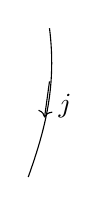
\begin{tikzpicture}[baseline=(current bounding box.center),x=0.9cm,y=0.9cm]
\draw (0.05,1.1).. controls (0.15,0.3) and (0,-0.3)..(-0.25,-1.0);
\draw[->] (0.05,0.35)--(-0.02,-0.16);
\node[right] at (0.04,0) {$j$};
\end{tikzpicture}
\end{adjustbox}
\tag{27}
\end{equation*}

(28)
\begin{center}
\begin{adjustbox}{max width=\linewidth}
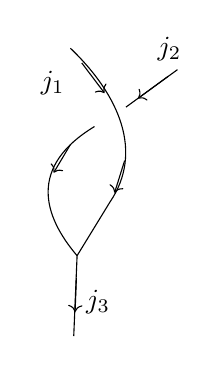
\begin{tikzpicture}[baseline=(current bounding box.center),x=0.85cm,y=0.85cm]
\draw (-0.45,2.2).. controls (0.28,1.5) and (0.65,0.65)..(0.14,-0.10)
 --(-0.35,-0.9)--(-0.40,-2.1);
\draw[->] (-0.28,1.98)--(0.06,1.53);
\draw[->] (0.36,0.52)--(0.21,0.04);
\draw[->] (-0.36,-1.23)--(-0.38,-1.74);
\draw (1.15,1.88)--(0.38,1.32);
\draw[->] (1.01,1.78)--(0.56,1.45);
\draw (-0.09,1.03).. controls (-1.08,0.43) and (-0.86,-0.30)..(-0.35,-0.9);
\draw[->] (-0.45,0.76)--(-0.70,0.34);
\node[left] at (-0.39,1.68) {$j_1$};
\node[above] at (1.03,1.87) {$j_2$};
\node[right] at (-0.36,-1.59) {$j_3$};
\end{tikzpicture}
\end{adjustbox}
$=$
\Unclear{GELFAND-P001466}{eq28-coefficient-j}{$(-1)^{j_1+j_2-j}q^{\frac{j(j+1)-j_1(j_1+1)-j_2(j_2+1)}{4}}$}
\begin{adjustbox}{max width=\linewidth}
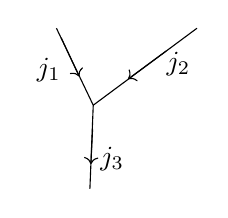
\begin{tikzpicture}[baseline=(current bounding box.center),x=0.85cm,y=0.85cm]
\draw (-0.55,1.15)--(0,0)--(-0.05,-1.25);
\draw (1.55,1.15)--(0,0);
\draw[->] (-0.48,1.01)--(-0.21,0.43);
\draw[->] (1.09,0.81)--(0.52,0.39);
\draw[->] (-0.01,-0.36)--(-0.035,-0.88);
\node[left] at (-0.34,0.53) {$j_1$};
\node[right] at (0.95,0.62) {$j_2$};
\node[right] at (-0.04,-0.80) {$j_3$};
\end{tikzpicture}
\end{adjustbox}
\end{center}

Это дает возм. строить инвар. зацеплений, кос,
заузленных ленточек.

\SourcePage{GELFAND-P001467}{66}
\underline{Инв. зацеплений.}

Фикс. ориентацию и направл. $t$.

(29)
\SourceFigure{GELFAND-P001467}{x58-y247-x646-y638}{Слева вертикальная стрелка вверх с подписью $t$. Справа криволинейная петля: верхний и нижний изгибы и два места в верхней средней части обведены овалами. Над левым средним местом стоит $m_i$, справа от петли --- $j$. На кривой видны стрелки; в средней части линии пересекаются, справа имеются разрывы. Точное прохождение ветвей и всех стрелок в наложенных штрихах не установлено.}

\underline{Элементарные фрагменты:}

1) фикс. точки, где нормаль $\parallel$ оси $t$ (выбранному напр.)

2) точки пересеч.

Расставляем числа $m_i$ в соединениях элем. фрагментов так, что
\begin{equation*}
-j\leq m_i\leq j \qquad (j\ \text{выб. любое})
\end{equation*}

\begin{equation*}
\sum_{\{m\}}\prod_{\substack{\text{по всем}\\\text{элем.}\\\text{фрагментам}}}
v(\{m\})=\varphi_{j_1\ldots j_k}(D_L,q)
\tag{30}
\end{equation*}
\Unclear{GELFAND-P001467}{x656-y1355-x935-y1489}{В (30) буква перед $(\{m\})$: $v$ или $\nu$.}

\textit{[От этой буквы отведён указатель к подписи:]} вычисл. выше матр. элементы

(31) \underline{Теорема}
\begin{equation*}
I_{j_1\ldots j_k}(L,q)
=q^{\sum_i N_+^i(D_L)-N_-^i(D_L)}\varphi_{\{j\}}(D_L,q)
\end{equation*}
\Unclear{GELFAND-P001467}{x1935-y1670-x2000-y1726}{[После $N_-^i(D_L)$ в показателе степени зачёркнут небольшой надстрочный знак; его чтение не установлено.]}

--- инвариант зацепления (не зав. от проекции узла на плоскость)

$N_\pm^i$ --- сколько раз $i$-я нитка прох. \underline{под} и \underline{над}

Здесь сод. инвар. Джонса.

Можно \Unclear{GELFAND-P001467}{x520-y2610-x734-y2730}{[Зачёркнутое слово неразборчиво]} строить инв. узлов по $\forall$ пр. алгебре Ли.

Есть гипотеза, что $SL_2$-инвариантов достаточно

Есть ещё $6j$-символы.

\SourcePage{GELFAND-P001468}{unlabelled}
\underline{25.4.88.}\quad\underline{Сем. Гельфанда}
\qquad
\underline{Ушверидзе}
\Unclear{GELFAND-P001468}{x1260-y33-x1400-y148}{[Зачёркнутые знаки неразборчивы]}
\underline{Александр Григорьевич.}
\Unclear{GELFAND-P001468}{x2040-y40-x2310-y150}{[Зачёркнутая запись неразборчива]}

\underline{Уравнение Риккати и квазиточнорешаемые задачи.}

\begin{equation*}
y'(\lambda)+y^2(\lambda)+2B(\lambda)y(\lambda)+C(\lambda)=0,
\tag{1}
\end{equation*}
\begin{equation*}
B(\lambda)=\sum_{\alpha=1}^N b_\alpha\Delta(\lambda-a_\alpha),
\tag{2}
\end{equation*}
\begin{equation*}
C(\lambda)=\sum_{\alpha=1}^N c_\alpha\Delta(\lambda-a_\alpha).
\tag{3}
\end{equation*}

Ищем решение (1) в виде
\begin{equation*}
y(\lambda)=\sum_{i=1}^M\Delta(\lambda-\lambda_i)
\tag{4}
\end{equation*}

Тогда при нек-рых
\textit{[вставка над строкой:]} условиях на $\Delta$
\Unclear{GELFAND-P001468}{x1000-y1240-x1248-y1328}{нахожд.}
\textit{[конец вставки]}
знач. параметров свод. к алгебр. ур-ям:
\begin{equation*}
\left\{
\begin{aligned}
&\sum_{i=1}^{M}{}'\Delta(\lambda_i-\lambda_k)
 +\sum_{\alpha=1}^{N}b_\alpha(\lambda_i-a_\alpha)=0\\
&\text{(сумма по }i\neq k\text{)}\\
&c_\alpha=2b_\alpha\sum_{i=1}^{M}\Delta(\lambda_i-a_\alpha)
\end{aligned}
\right.
\tag{5}
\end{equation*}
\Unclear{GELFAND-P001468}{x350-y1390-x1615-y1675}{[В первой строке (5) после $b_\alpha$ непосредственно стоят $(\lambda_i-a_\alpha)$; в первом суммировании написано $i=1$, в аргументе $\Delta$ --- $\lambda_i-\lambda_k$. Так в источнике.]}

(6) \underline{Св-ва $\Delta$ и $\Omega$}
\qquad (обобщ. теор. слож. для элл. ф-й)

\begin{equation*}
\begin{aligned}
1)\quad &\Delta(\lambda_1)\Delta(\lambda_2)+\Delta(\lambda_2)\Delta(\lambda_3)
+\Delta(\lambda_3)\Delta(\lambda_1)\\
&\qquad +\Omega(\lambda_1)+\Omega(\lambda_2)+\Omega(\lambda_3)=0\\
&\text{при }\lambda_1+\lambda_2+\lambda_3=0
\end{aligned}
\end{equation*}
\begin{equation*}
2)\quad \Delta(\lambda)+\Delta(-\lambda)=0
\end{equation*}

3) \Unclear{GELFAND-P001468}{x435-y2450-x570-y2578}{[Зачёркнутая формула; различим знак, похожий на $\Delta$, остальное не установлено]}
$\Omega(\lambda)-\Omega(-\lambda)=0$

(7) \underline{Примеры решений сист. (6)}

\begin{equation*}
1)\quad \Delta(\lambda)=\frac{1}{\lambda},\qquad \Omega(\lambda)=0;
\end{equation*}
\Unclear{GELFAND-P001468}{x1335-y2810-x1494-y2960}{[Справа от первой пары формул зачёркнуты знаки; различим треугольный знак, похожий на $\Delta$.]}

\begin{equation*}
2)\quad \Delta(\lambda)=\omega\operatorname{ctg}\omega\lambda,
\qquad \Omega(\lambda)=\frac{\omega^2}{3}
\end{equation*}
\begin{equation*}
3)\quad \Delta(\lambda)=\zeta(\lambda),
\qquad \Omega(\lambda)=\zeta^2(\lambda)-\wp(\lambda)
\end{equation*}
\textit{[Под $\zeta(\lambda)$, с коротким указателем:]} ф-я Вейерштрасса
\qquad (квазиперио

\SourcePage{GELFAND-P001469}{67}
\underline{Прилож.}

А. $y=\dfrac{f'}{f}\quad\Rightarrow$ ур-е Шредингера для $f$;

Решение (6) с сингулярностью в $0$ удовлетворяет ур-ю
\begin{equation*}
\Delta'(\lambda)+\Delta^2(\lambda)=2\Omega(\lambda)+\Omega(0)
\tag{8}
\end{equation*}

\begin{center}
\begin{adjustbox}{max width=\linewidth}
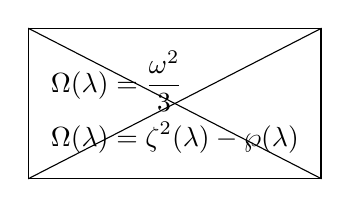
\begin{tikzpicture}
\node[draw,inner sep=8pt] (cancelled) at (0,0) {$\begin{aligned}
\Omega(\lambda)&=\frac{\omega^2}{3}\\
\Omega(\lambda)&=\zeta^2(\lambda)-\wp(\lambda)
\end{aligned}$};
\draw (cancelled.north west) -- (cancelled.south east);
\draw (cancelled.south west) -- (cancelled.north east);
\end{tikzpicture}
\end{adjustbox}
\end{center}

(9) $\Delta_0(b\lambda)+a\lambda$ --- общее решение сист. (6), где

$\Delta_0$ --- одна из ф-й примера (6)
\Unclear{GELFAND-P001469}{x438-y860-x2110-y1115}{[В (9) перед $\Delta_0(b\lambda)$ внешнего множителя нет; в следующей строке написано «примера (6)». Так в источнике.]}

Б. Отсюда ещё получ. реш. Бете-анзаца для спин. систем.

В. $(5)\Leftrightarrow$
\textit{[вставка над строкой:]} в случае
\Unclear{GELFAND-P001469}{x825-y1238-x1030-y1340}{[Зачёркнутая запись перед $(7)_1$ неразборчива]}
$(7)_1$ \textit{[конец вставки]}
усл. равновесия классич. сист. заряж. частиц, к-рых
\underline{2 сорта:} неподв. частицы с коорд. $a_\alpha$ и зарядами $b_\alpha$;
подвижные с
\Unclear{GELFAND-P001469}{x800-y1425-x1005-y1558}{[Зачёркнутое слово неразборчиво; над ним вписано «коорд.»]}
$\lambda_i$ и зарядом $1$.

\textit{[Справа:]} \underline{Потенциал:}
$q_iq_k\ln|\lambda_i-\lambda_k|$

В случае $(7)_2$
частицы на окружности с потенциалом
\begin{equation*}
q_iq_k\ln|\sin(\lambda_i-\lambda_k)|
\end{equation*}

В случае $(7)_3$ потенц. взаимодействия
\begin{equation*}
q_iq_k\ln\theta(\lambda_i-\lambda_k)
\end{equation*}

(10) \underline{Для ур-я Шредингера}

$\lambda_i$ --- узлы волновой ф-и

В кулоновской сист.

\Unclear{GELFAND-P001469}{x500-y2640-x570-y2745}{[Перед $\lambda_i$ зачёркнут знак; его чтение не установлено]}
$\lambda_i$ --- коорд. заряж. частиц

В ур-и Бете $\lambda_i$ --- быстроты

\begin{center}
\rule{2cm}{0.4pt}\quad$\cdot$\quad\rule{2cm}{0.4pt}
\end{center}

Устойчивость квантовомех. сист. $\Leftrightarrow$ устойч. кулоновской системы

\begin{center}
\rule{2cm}{0.4pt}\quad$\cdot$\quad\rule{2cm}{0.4pt}
\end{center}

\underline{Что делать с частичной интегрируемостью?}
(с неполн. сист. интегралов)

\begin{equation*}
H=H_0+L_1(H_1-c_1)+L_2(H_2-c_2),
\qquad L_j\text{ --- операторы}
\tag{11}
\end{equation*}
Пусть $H_j$ коммутируют $j=0,1,2$.

\SourcePage{GELFAND-P001470}{unlabelled}
\Unclear{GELFAND-P001470}{top-left-label}{[зачёркнутая помета на левом поле; неразборчиво]}

Рассм. общ. соб. вектор $H_0,H_1,H_2$; тогда
\Unclear{GELFAND-P001470}{top-line-cancellation}{[зачёркнуто; неразборчиво]}

Если $c_j$ — соб. знач. $H_j$, то по ним строится соб. знач.
\Unclear{GELFAND-P001470}{top-right-cancellation}{[зачёркнуто; неразборчиво]} $H$
(и \Unclear{GELFAND-P001470}{top-eigenvectors-verb}{знаем} соб. вект. — \underline{столько, какова} кратность вырождения)

На этом языке
\begin{equation*}
\begin{aligned}
\text{квант. нелин. Шредингер}&\ \Longleftrightarrow\ \text{гарм. осциллятору}\\
\text{[зачёркнуто: опер.] энергия}&\ \Longleftrightarrow\ \text{опер. числа частиц}
\end{aligned}
\end{equation*}

\begin{center}— . —\end{center}

Спектр $H_i$ нах. из ур-й анзаца Бете

\begin{center}— . —\end{center}

\underline{Ссылка:}

Краткие сообщ. по физике ФИАН.

\underline{Переход от ур-я Риккати к ур-ю Шредингера}

Это можно бесчисл. кол-вом способов
\begin{equation*}
y=\frac{f'}{f}\quad\Longrightarrow
\end{equation*}
\begin{equation*}
f''+2Bf'+Cf=0
\qquad\text{(незав. перем. здесь $\lambda$)}
\tag{12}
\end{equation*}

Умножим [вставлено над строкой: (12)] на произвольную ф-ю $A$ и потом избавл. от $f'$
$\Longrightarrow$ [под строкой: (заменой независ. перем.!)]
$\Longrightarrow$ получ. ур-е Шредингера
\begin{equation*}
\left[-\frac{\partial^2}{\partial x^2}+V(x)\right]\Psi(x)=0
\tag{13}
\end{equation*}

По каждому $A$ получ. свой потенциал $V$.

Ф-ю $A$ можно подобрать так, чтобы информация о числах
\Unclear{GELFAND-P001470}{lower-number-cancellation}{[зачёркнуто; неразборчиво]}
$c_\alpha,\lambda_i$ сосредот. в не зав. от $x$ части потенциала:
\begin{equation*}
V(x)=U(x)-E(\lambda_i)
\tag{14}
\end{equation*}

Тогда (13) \Unclear{GELFAND-P001470}{lower-equation-cancellation}{[зачёркнуто; неразборчиво]}
$\sim$ ур-ю Шредингера

Для этого нужно, чтобы было
\begin{equation*}
A(\lambda)=\prod_{\alpha=1}^{N}\Xi(\lambda-a_\alpha),
\qquad\frac{\Xi'(\lambda)}{\Xi(\lambda)}=\Delta(\lambda)
\tag{15}
\end{equation*}

Переход к $x$;
\begin{equation*}
x=\int^{\lambda(x)}\frac{d\lambda}{\sqrt{A(\lambda)}}
\tag{16}
\end{equation*}

\SourcePage{GELFAND-P001471}{68}
(17) \Unclear{GELFAND-P001471}{top-initial-cancellation}{[зачёркнуто; неразборчиво]}
В случае $(7)_1$:
\begin{equation*}
A(\lambda)=\prod_{\alpha=1}^{N}(\lambda-a_\alpha)
\end{equation*}
\Unclear{GELFAND-P001471}{top-line-cancellation}{[зачёркнуто: лин. ф-я от $\lambda$]}

($\Xi$ — лин. ф-я от $\lambda$)

отсюда получ. преобр. Якоби (16)

\underline{Использ. кулон. аналогию для классификации}
точно реш. и квазиточно решаемых зад.

Пусть $N=2$ в (2)–(3)

\begin{center}
\begin{adjustbox}{max width=\linewidth}
\begin{tikzpicture}[x=1cm,y=1cm]
\draw (0,0) -- (5.2,0);
\draw (1.2,-0.10) -- (1.2,0.10);
\draw (3.2,-0.10) -- (3.2,0.10);
\node[above] at (1.2,0.20) {$b_1$};
\node[above] at (3.2,0.20) {$b_2$};
\node[below] at (1.2,-0.15) {$a_1$};
\node[below] at (3.2,-0.15) {$a_2$};
\node[right] at (5.35,-0.28) {$\lambda$};
\end{tikzpicture}
\end{adjustbox}
\end{center}

$a_1,a_2$ — коорд. неподв. частиц (классических)

Подв. частицы $\underset{\text{коорд.}}{\{\lambda_i\}}$ — их $M$ штук

(18) \Unclear{GELFAND-P001471}{middle-potential-cancellation}{[зачёркнуто; неразборчиво]}
Потенц. $V$ не содержит $M$ (!) $\Longrightarrow$ имеем точно реш. модель.

(19) Пусть $b_1,b_2>0$

\begin{center}
\begin{adjustbox}{max width=\linewidth}
\begin{tikzpicture}[x=1cm,y=1cm]
\draw (0,0) -- (4.2,0);
\draw (0,-0.16) -- (0,0.18);
\draw (4.06,-0.18) -- (4.22,0.19);
\node[above] at (0,0.22) {$b_1$};
\node[above] at (4.2,0.22) {$b_2$};
\draw (1.08,-0.12) -- (1.10,0.17);
\draw (1.62,-0.13) -- (1.68,0.16);
\draw (2.12,-0.13) -- (2.20,0.12);
\draw (2.47,-0.13) -- (2.56,0.12);
\draw (2.85,-0.13) -- (2.95,0.10);
\draw (3.25,-0.15) -- (3.37,0.17);
\end{tikzpicture}
\end{adjustbox}
\end{center}

Частицы внутри не выйдут из-за отталкивания
$\Longrightarrow\ \exists\min\ \Longrightarrow\ \exists$ реш. ур-я Шредингера
с $M$ узлами $\Longrightarrow$ интегрируемость!!!

(находятся все волн. ф-и!!)

Другой случай

(20)
\begin{center}
\begin{adjustbox}{max width=\linewidth}
\begin{tikzpicture}[x=1cm,y=1cm]
\draw (0,0) -- (7.0,0);
\fill (1.0,0) circle (0.075);
\draw (3.0,0) circle (0.065);
\node[above] at (1.0,0.20) {$-$};
\node[above] at (3.0,0.20) {$+$};
\draw (3.92,-0.14) -- (3.94,0.10);
\draw[<-] (4.12,0) -- (4.32,0);
\draw (4.55,-0.15) -- (4.55,0.17);
\draw (5.00,-0.13) -- (5.08,0.13);
\draw (6.10,-0.14) -- (6.18,0.18);
\draw (6.52,-0.11) -- (6.54,0.10);
\draw (7.06,-0.16) -- (7.14,0.14);
\node[below] at (5.85,-0.24) {$M$ частиц};
\end{tikzpicture}
\end{adjustbox}
\end{center}
\SourceFigure{GELFAND-P001471}{diagram20-faint-strokes}{В схеме (20) левый конец горизонтальной линии утолщён и снабжён наклонными штрихами; уверенно выделить наконечник стрелки нельзя. Под этим концом и под левой тёмной точкой видны слабые штрихи вниз влево; их точное назначение и связь с жирными штрихами неясны.}
\Unclear{GELFAND-P001471}{margin-below20}{[на левом поле под (20): короткий отдельный наклонный штрих]}

Усл. устойчивости системы $M$ частиц справа от $b_2$:
\begin{equation*}
\underline{b_1+b_2+M<0}
\tag{21}
\end{equation*}

(не подх. к $b_2$, но и не уходят на $\infty$)

Но это усл. нарушится при большом $M$!
$\Longrightarrow$ возникает лишь конеч. число уровней.

\SourcePage{GELFAND-P001472}{unlabelled}
Выбирая по разному интервалы, получим разные задачи.

Здесь получ. точно реш. модели (магнетики).

\underline{\underline{Бейлинсон А.}}

\underline{о раб. \Unclear{GELFAND-P001472}{upper-atiya-name}{Ати}}

\underline{Новые инварианты 3-х и 4-хмерных мн-зий}

(полубеск. теор. Морса)

\begin{equation*}
\underset{\substack{\text{естеств.}\\\infty\text{-мерн. мн-зия}}}{X}
\overset{f}{\longrightarrow}\mathbb{R}
\qquad\text{— морсовская ф-я.}
\end{equation*}

Критич. точки будут сод. $\infty$ число $+$ и $-$ квадратов, но
у разных точек отличие — на конечное число.

Возникают новые гомологии.

На мн-зии $X$ зададим рим. метрику

Пусть сначала $\dim X<\infty$ и $X$ компактно

$g$ — метрика,
\begin{equation*}
\tau=\operatorname{grad}f
\end{equation*}

Рассм. \Unclear{GELFAND-P001472}{middle-flow-cancellation}{[зачёркнуто; неразборчиво]}
[вставлено над строкой: траектории] поля $\tau$

Они 2-х типов: точки [под строкой: (крит.)] и траект., соединяющие 2 крит. точки.

Если метрика — общего положения, то рассм. пр-во $T(x_1,x_2)$
всех траект., идущих из $x_1$ в $x_2$. Тогда
\begin{equation*}
\dim T(x_1,x_2)=\operatorname{ind}_{x_1}f-\operatorname{ind}_{x_2}f-1
\tag{1}
\end{equation*}

В частности, \underline{если индексы отл. на 1, то дискретное мн-во.}

Пусть
\begin{equation*}
\operatorname{ind}_{x_1}f=\operatorname{ind}_{x_2}f+1
\tag{2}
\end{equation*}

Тогда с $\forall$ траект., соед. $x_1$ и $x_2$, связывают число $\pm1$,
завис. от данных ориентац.
\Unclear{GELFAND-P001472}{bottom-orientation-cancellation}{[зачёркнуто; неразборчиво]}
[вставлено над строкой: $T(x_1,x_2)$] Теперь строим комплекс

\SourcePage{GELFAND-P001473}{69}
\begin{equation*}
\longrightarrow C_i\overset{d}{\longrightarrow}C_{i-1}\longrightarrow\ldots
\tag{3}
\end{equation*}

$C_i$ — вект. пр-во с базисом $\{x_\alpha\}$, $\operatorname{ind}x_\alpha=i$

$d$ зад. матрицей;

индекс элем. = пара точек соседн. индекса $x_1,x_2$
\begin{equation*}
d=\Vert d_{x_1x_2}\Vert,
\end{equation*}
\begin{equation*}
d_{x_1x_2}=\sum_{\substack{\text{траект.,}\\\text{соед. }x_1,x_2}}\pm1
\tag{4}
\end{equation*}

\begin{center}
\rule{12mm}{0.4pt}\quad$\cdot$\quad\rule{12mm}{0.4pt}
\end{center}

Пусть $M$ — 3-мерное компактное мн-ие.

Рассм. пр-во всех [вставка над строкой: неприводимых] связностей $C$
[зачёркнуто: \Unclear{GELFAND-P001473}{mid-cancelled-after-c}{неразборчиво}]

[Под словом «связностей»: (эрмитовых)]

на тривиальном 2-мерном расслоении на $M$

Такая связность имеет вид $d+A$, где
\begin{equation*}
A\in\Omega^1(M)\otimes\mathrm{su}_2
\end{equation*}

Будем их рассм. с точн. до калибр. эквивалентности
\begin{equation*}
G\text{ — калибр. группа }SU_2^M;\qquad
X=C/G\text{ — пр-во орбит}
\end{equation*}
$X$ — основное мн-ие.

На $X$ зададим ф-ю Морса, точнее её дифференциал
$\nu$ — 1-форму на $C$.

% В источнике слова «Касат. вектор к C» подчёркнуты волнистой линией.
\underline{Касат. вектор к $C$}: матричнозначная 1-форма

($C$ — аффинное пр-во)
\begin{equation*}
B\in\Omega^1(M)\otimes\mathrm{su}_2.
\end{equation*}
\begin{equation*}
\langle\nu,B_\nabla\rangle
=\int_M\operatorname{Tr}(F_\nabla\cdot B),
\qquad B\in\Omega^1(M)\otimes\mathrm{su}_2
\tag{5}
\end{equation*}
[Под $F_\nabla$ с указателем: кривизна $A$]

[Справа:] $F_\nabla\cdot B$ — внешнее произв-о, (3-форма !!)
\begin{equation*}
F_\nabla=dA+\frac{1}{2}[A,A]
\tag{6}
\end{equation*}

\SourcePage{GELFAND-P001474}{unlabelled}
% В источнике «Св-ва ν» подчёркнуто волнистой линией.
(7) \underline{Св-ва $\nu$}.

1. $\nu$ поднимается с $X$

2. $\nu$ — замкнутая 1-форма

3. [Вставка над строкой перед $\nu$: Первообр.] $\nu$ — вторичный хар. класс для
\Unclear{GELFAND-P001474}{upper-class-symbol}{$c_2$} (кл. Чжена)

— класс Черна-Саймонса для $c_2$:
\begin{equation*}
\int_{M\times[0,1]}\operatorname{Tr}(F_{\widetilde\nabla})^2
\tag{8}
\end{equation*}
где

(9) [Зачёркнуто: \Unclear{GELFAND-P001474}{mid-cancelled-notation}{$A_\nabla$}]
$\widetilde\nabla$ — связность на трив. расслоении на $M\times[0,1]$

с потенциалом в точке $(x,t)$, равным $tA$.

Эта связность на $C$, а не на $X$.

[Мелкая вставка между строками:]
\underline{Замеч. \Unclear{GELFAND-P001474}{mid-remark-initials}{И. М. Г.}}:
Это все сод. в «простой» части раб. Габр.-Гельф.-Лосик

Посмотрим на критич. точки.

[Зачёркнута короткая строка:
\Unclear{GELFAND-P001474}{mid-cancelled-line}{неразборчиво}]

Это связности с кривизной 0, т.е. интегрируемые, т.е.
представления $\pi_1(M)$

% В источнике «Гессиан» подчёркнут волнистой линией.
\underline{Гессиан}.
\begin{equation*}
\nabla\in C,\qquad
T_{C,\nabla}=\Omega^1(M)\otimes\mathrm{su}_2
\overset{\text{проекция}}{\longrightarrow}T_{X,\overline\nabla}
\tag{10}
\end{equation*}
Введем

[Номер формулы переправлен:
(\Unclear{GELFAND-P001474}{lower-equation-label}{11})]
\begin{center}
\Unclear{GELFAND-P001474}{lower-m-x-notation}{$\nabla_{ad}:\Omega^0(X)\otimes\mathrm{su}_2
\longrightarrow\Omega^1(X)\otimes\mathrm{su}_2,$}
\end{center}
по ф-ле
\begin{equation*}
\nabla_{ad}(\varphi)=d\varphi+[A,\varphi]
\tag{12}
\end{equation*}
и тогда
\begin{equation*}
T_{X,\nabla}=
\frac{\Omega^1(X)\otimes\mathrm{su}_2}
{\nabla_{ad}\bigl(\Omega^0(X)\otimes\mathrm{su}_2\bigr)}
\tag{13}
\end{equation*}
Это верно для любой связности.


\SourcePage{GELFAND-P001475}{70}
Гессиан — квадр. форма на пр-ве (13), инвар.
опред. в крит. точке.
\begin{equation*}
H(\varphi)=\int_M\operatorname{Tr}(\nabla_{ad}\varphi\cdot\varphi),
\qquad \varphi\in T_{X,\nabla}, \tag{14}
\end{equation*}
\begin{equation*}
\Omega^1(M)\otimes\mathrm{su}_2
\overset{\nabla_{ad}}{\longrightarrow}
\Omega^2(M)\otimes\mathrm{su}_2. \tag{15}
\end{equation*}
Если связность была интегрир., то $\nabla_{ad}$ — комплекс
([зачёркнут знак:
\Unclear{GELFAND-P001475}{complex-cancel}{$\varphi$ / $\Phi$ / неразборчиво}]
$\nabla_{ad}^{2}=0$)
корректно опред. $\nabla_{ad}\varphi$ (не зависит от представителя
в факторе (13))

\underline{ф-я} [вставлено над строкой:
\Unclear{GELFAND-P001475}{morse-function-insert}{$\int\nu$ / $\int v$}]
\underline{— морсовская} $\Longleftrightarrow$ $\nabla_{ad}$ не имеет
1-мерных когомологий, т.е.
\begin{equation*}
H^1(M,\text{любое предст. }\pi_1)=0 \tag{16}
\end{equation*}
[Под словами «любое предст. $\pi_1$» дописано: «или $\forall$ лок. сист.»]

Это равносильно тому, что
\begin{equation*}
M\text{ — гомологич. сфера, т.е. }H_1(X,\mathbb Z)=0 \tag{17}
\end{equation*}
\Unclear{GELFAND-P001475}{homology-equivalence}{[В (17) написано $X$; утверждение о равносильности сохранено по источнику.]}

По станд. схеме надо рассм. градиентные потоки.

2 крит. точки $\longleftrightarrow$ 2 предст. $\pi_1$.

Соед. их траекторией из неинтегрир. связностей.

В окр. кривой выб. единую коорд. систему
\begin{center}
\begin{adjustbox}{max width=\linewidth}
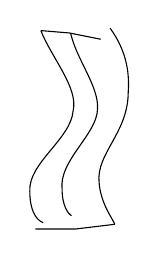
\begin{tikzpicture}[x=1cm,y=1cm]
\draw (0.04,2.50) .. controls (0.18,2.15) and (0.52,1.77) .. (0.45,1.48)
 .. controls (0.42,1.12) and (-0.12,0.82) .. (-0.10,0.46)
 .. controls (-0.10,0.23) and (-0.03,0.10) .. (0.07,0.06);
\draw (0.92,2.53) .. controls (1.11,2.27) and (1.17,2.00) .. (1.15,1.72)
 .. controls (1.15,1.20) and (0.74,0.94) .. (0.78,0.57)
 .. controls (0.80,0.31) and (0.94,0.13) .. (0.98,0.04);
\draw (0.04,2.50) -- (0.40,2.47) -- (0.80,2.39);
\draw (0.42,2.46) .. controls (0.50,2.12) and (0.78,1.79) .. (0.76,1.50)
 .. controls (0.75,1.18) and (0.27,0.85) .. (0.31,0.49)
 .. controls (0.31,0.27) and (0.39,0.17) .. (0.43,0.15);
\draw (-0.03,-0.02) -- (0.48,-0.02) -- (0.98,0.04);
\end{tikzpicture}
\end{adjustbox}
\end{center}
и следим за изменением матр. 2-х производных.
\begin{equation*}
\begin{aligned}
\text{Разница [вставлено: индексов]}&=
\text{числу точек [вставлено: на пути], когда возникает 0-я мода}\\
&=\text{спектр. асимметрия.}
\end{aligned}\tag{18}
\end{equation*}
Это делается с
\Unclear{GELFAND-P001475}{index-theorem-cancel}{[зачёркнутое слово неразборчиво]}
пом. обычн. теор. об индексе.
\begin{equation*}
\text{Разность индексов, }\underline{\mathrm{mod}\ 8},\quad
\text{корректно определена!!} \tag{19}
\end{equation*}

\SourcePage{GELFAND-P001476}{unlabelled}
\underline{Следующий пример.}

Вычисл. индекса с точки зрения конечномерной ситуации.
(Тоже для гомологич. сферы).

\begin{center}
\begin{adjustbox}{max width=\linewidth}
\begin{tikzpicture}[x=1cm,y=1cm]
\node at (0,1.4) {$N$};
\node[anchor=west] at (0.45,1.4) {— симплектич. мн-зие};
\node[rotate=-35] at (-0.50,0.68) {$\cup$};
\node[rotate=25] at (0.50,0.68) {$\cup$};
\node at (-0.95,0) {$L_1$};
\node at (0.90,0) {$L_2$};
\node[anchor=west] at (1.30,0) {— лагранжевы подмн-зия};
\node[anchor=east] at (-1.60,0.7) {(20)};
\end{tikzpicture}
\end{adjustbox}
\end{center}
Пусть
\begin{equation*}
L_1\cap L_2\quad\text{конечно.}\tag{21}
\end{equation*}
Хотим вычислить взвешенное число точек пересеч.

(22) \underline{Пример.} $N=$
\Unclear{GELFAND-P001476}{cotangent-cancel}{[зачёркнуто: $\Omega$ / неразборчивый знак]}
$T^*L$,
\begin{center}
\begin{adjustbox}{max width=\linewidth}
\begin{tikzcd}[column sep=large]
L_1=L \arrow[r,hook,"{\text{0-е сеч.}}"] & N &
L=L_2 \arrow[l,hook',"df"]
\end{tikzcd}
\end{adjustbox}
\end{center}
[Под $L_1=L$ зачёркнуто:
\Unclear{GELFAND-P001476}{below-section-cancel}{$H_2$ / $L_2$ / неразборчиво}.]
$f$ — морсовская

$L_1\cap L_2$ — крит. точки $f$

пересеч. трансверсально.

точке пересеч. — индекс
\begin{equation*}
L_1\cap L_2\overset{\mathrm{index}}{\longrightarrow}
\{0,1,\ldots,\dim L\}
\end{equation*}
\begin{equation*}
\chi(N)=\sum_{x\in L_1\cap L_2}(-1)^{\mathrm{index}\,x}\tag{23}
\end{equation*}
\underline{Общая ситуация (20)}: опред. относительный индекс!

(24) $X$ — пути, соед. $L_1$ и $L_2$
\begin{equation*}
\begin{aligned}
[0,1]&\longrightarrow N\\
0&\longrightarrow L_1\\
1&\longrightarrow L_2
\end{aligned}
\end{equation*}
На таком $X$ есть многозначная ф-я Морса

Крит. точки — точки пересеч. $L_j$

$\varphi\in X$, $\tau$ — кас. вектор в $\varphi$, т.е. векторное поле вдоль $\varphi$

[От $\varphi$ проведена вниз короткая черта к подписи «путь».]

\SourcePage{GELFAND-P001477}{71}

Тогда
\begin{equation*}
\langle \nu,\tau\rangle := \int_0^1 \omega(\dot{\varphi},\tau),
\tag{25}
\end{equation*}
\Unclear{GELFAND-P001477}{one-form-symbol}{Знак, переданный как $\nu$, может быть латинским $v$; тот же знак стоит ниже перед «морсовская».}

где

$\omega$ — симп. форма.

$\nu$ — морсовская, если $L_1$ и $L_2$ пересек. трансверсально.

Разность индексов опред., но есть и элем. конструкция

(через индекс Маслова)

Рассм. мн.-ие $M$ — гомол. сфера. !

(26) \underline{Теорема}

$M$ можно разрезать по рим. поверхности $Z$,

(разбиение Хегора)

$$
W=W_1\cup W_2,\qquad \partial W_i=Z.
$$
\Unclear{GELFAND-P001477}{decomposition-letter}{В формуле написано $W$, тогда как в предшествующем тексте — $M$; отношение обозначений не пояснено.}

(27)
\begin{center}
\begin{adjustbox}{max width=\linewidth}
\begin{tikzcd}[row sep=small,column sep=large]
& \pi_1(W_1) \arrow[dr] & \\
\pi_1(Z) \arrow[ur] \arrow[dr] & & \pi_1(M) \\
& \pi_1(W_2) \arrow[ur] &
\end{tikzcd}
\end{adjustbox}
\end{center}

общим опред. $\pi_1(M)$

$\pi_1(W_j)$ — своб. группа с $g$ образующими

Предст. $\pi_1(M)$ [зачёркнуто: \Unclear{GELFAND-P001477}{cancelled-representation-word}{одно неразборчивое слово}]
— в нем $\pi_1(W_j)$ — лагранжевы мн.-ия.

Рассмотрим

(28)
\SourceFigure{GELFAND-P001477}{cylinder-decomposition}{Горизонтальный рисунок: две выпуклые наружные части соединены сверху и снизу почти прямыми линиями; у соединений видны дуги, частью слабые. Над левой частью стоит $W_1$, над правой — $W_2$, под средней частью — «цилиндр». Короткие наклонные штрихи у верхних соединений не позволяют уверенно установить, являются ли они стрелками или частью контура.}

[зачёркнуто: \Unclear{GELFAND-P001477}{cancelled-before-path}{одно неразборчивое слово перед «Путь»}]
Путь — сем-во связностей.

2-я половина раб.:

замена плоских связностей на инстантоны,

переход к $M^4$ и

инварианты Дональдсона

($M^4$ разрезается на 2 трёхмерных).
\Unclear{GELFAND-P001477}{four-dimensional-cut}{Фраза «$M^4$ разрезается на 2 трёхмерных» передана буквально; размерностный смысл не уточнён.}

\SourcePage{GELFAND-P001478}{unlabelled}

\underline{12.9.88 г.}\qquad \underline{\underline{Сем. Гельфанда.}}

1. «В пр-ве какого наименьшего числа измерений две двумерные плоскости
могут скрещиваться?»

2. \underline{\underline{Что такое детерминант?}}

2 ур-я 1-го пор. можно заменить [вставлено над строкой: одним]
ур-ем 2-го порядка. Как?

\begin{equation*}
\begin{cases}
\left(\dfrac{d}{dx}+q_{11}\right)\varphi_1+q_{12}\varphi_2=0\\
q_{21}\varphi_1+\left(\dfrac{d}{dx}+q_{22}\right)\varphi_2=0
\end{cases}
\tag{1}
\end{equation*}

а) \underline{1-й способ}: выражаем из 1-го $\varphi_2$ и подст. во 2-е

\underline{2-й способ}: выражаем из 2-го $\varphi_1$ и подст. в 1-е

Получ. разные ур-я!

но решив одно, можно решить 2-е.

Это известно под назв. «преобразование Бэклунда».

Можно взять лин. комб. $\varphi_1$ и $\varphi_2$ и тогда возник. семейство ур-й.

Ответы очень красивые

б) Что для 3-х ур-й 1-го порядка?

Это уже сложнее и красота пропадает.

Сделали Гельфанд и Ретах.

Есть раб. Сато, Кашивары о некоммут. определителях.

в) Пусть $q_{ij}=\mathrm{const}$

[слева зачёркнуто: \Unclear{GELFAND-P001478}{cancelled-margin-label}{неразборчивый знак пункта с правой скобкой}]
Тогда есть детерминант

\begin{equation*}
\begin{vmatrix}
\dfrac{d}{dx}+q_{11}&q_{12}\\
q_{21}&\dfrac{d}{dx}+q_{22}
\end{vmatrix}
=\left(\frac{d}{dx}\right)^2+(q_{11}+q_{22})\frac{d}{dx}
+(q_{11}q_{22}-q_{12}q_{21})
\tag{2}
\end{equation*}

$$
\frac{d}{dx}\longleftrightarrow\lambda
\qquad\Longrightarrow\qquad\text{получ. характ. опред. матрицы}
$$

в общем случае получ. [вставлено над строкой: (некоммут. аналог)]
характеристич. определителя.

$$
\begin{vmatrix}
a_{11}&a_{12}\\
a_{21}&a_{22}
\end{vmatrix}
\quad\text{— ?}
$$

$a_{ij}$ — отображение $E_j\to E_i$,

так что $a_{11}a_{22}-a_{12}a_{21}$ не имеет смысла.

Всего 4 определителя:

\begin{equation*}
a_{11}-a_{12}a_{22}^{-1}a_{21}
\tag{3}
\end{equation*}

[зачёркнуто: \Unclear{GELFAND-P001478}{cancelled-final-symbol}{один знак, похожий на $a$ или «и»}]
и т.п.

\SourcePage{GELFAND-P001479}{84}

3-й порядок: 36 способов записи.

Возникает некоммут. $K$-теория и некоммут. гомологии.

\Unclear{GELFAND-P001479}{overwritten-section-label}{в) / г)}
8 букв расположены кубиком $2\times2\times2$

Что такое определитель?

Это сделал Кэли.

Считалось, что после Гильберта результаты Гордана, Кэли, Клебша и др.
потеряли интерес. Они были объявлены старомодной чепухой. Но это
неверно.

\underline{\underline{Мур.}}\quad (\underline{GREGORY MOORE})\quad (\underline{I,AS. Princeton})

\underline{Конформная} \underline{теория} \underline{поля.}\quad (CFT)

Модель Изинга

\begin{center}
\begin{adjustbox}{max width=\linewidth}
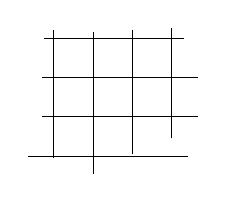
\begin{tikzpicture}[scale=0.5]
\draw (0,-0.05)--(0,3.2);
\draw (1,-0.45)--(1,3.15);
\draw (2,0.05)--(2,3.2);
\draw (3,0.45)--(3,3.25);
\draw (-0.25,3)--(3.3,3);
\draw (-0.3,2)--(3.65,2);
\draw (-0.3,1)--(3.65,1);
\draw (-0.65,0)--(3.4,0);
\end{tikzpicture}
\end{adjustbox}
\end{center}

2-мерн. решётка, в $\forall$ точке — переменная $\sigma :=$
[зачёркнуто: \Unclear{GELFAND-P001479}{cancelled-spin-value}{короткая запись, закрытая плотными косыми штрихами}] $\pm1$

[под словом «решётка»: (квадратная)]

\begin{equation*}
\text{Энергия}\quad E=\sum_{\langle ij\rangle}\sigma_i\sigma_j
\tag{1}
\end{equation*}

$\langle ij\rangle$ — соседние точки

Статсумма

\begin{equation*}
Z=\sum e^{-\beta E}
\tag{2}
\end{equation*}

\SourceFigure{GELFAND-P001479}{ising-cylinder}{Вертикальный цилиндр: замкнутый верхний овал, две боковые линии и нижняя дуга. Внутри идут несколько почти вертикальных линий; внизу видны короткий наклонный штрих слева и поперечный штрих правее. Точное соединение внутренних линий и значение коротких штрихов неясны; подписей у рисунка нет.}

Рассм. на цилиндре и измельчаем решётку

Асимптотика выраж. через ф-и

[слева зачёркнуто: \Unclear{GELFAND-P001479}{cancelled-before-eta}{знак, похожий на $Z$, и следующие неразборчивые штрихи}]

$$
\eta(\tau)=q^{1/24}\prod(1-q^n),\qquad q=e^{i\pi\tau}
$$
\Unclear{GELFAND-P001479}{eta-q-normalization}{В источнике $q=e^{i\pi\tau}$ вместе с $q^{1/24}\prod(1-q^n)$; согласование нормировок не уточнено.}

$$
\theta_3(\tau)=\sum e^{i\pi\tau n^2}
$$

и аналог. $\theta_2,\theta_4$

[над строкой: $\tau=i\beta$]

Инвар. относительно замены

$$
\tau\longrightarrow-1/\tau
$$

$$
Z\longrightarrow
\left|\frac{\theta_2}{\eta}\right|
+\left|\frac{\theta_3}{\eta}\right|
+\left|\frac{\theta_1}{\eta}\right|
\qquad\text{(с точн. до множителя)}
$$
\Unclear{GELFAND-P001479}{last-theta-index}{Последний индекс наиболее похож на $1$; возможно $4$. Выше отдельно написано $\theta_2,\theta_4$.}

$$
Z(\beta)=Z\left(\frac{1}{\beta}\right)
$$

\SourcePage{GELFAND-P001480}{unlabelled}
In CFT we associate real analytic functions
to surfaces

\SourceFigure{GELFAND-P001480}{top-torus-cycles}{Тор с отверстием; внизу дуга с подписью $\alpha$, справа поперечная дуга с подписью $\beta$. Виден наконечник влево на нижней дуге и наконечник вниз-вправо у наружного контура. Штрихи около верхнего края отверстия и разрывы поперечной дуги требуют сверки с оригиналом.}
$$
=\sum_{i=1}^{N} f_i(\tau)\bar g_i(\tau),\qquad
f_i:=\left\{\sqrt{\frac{\theta_2}{\eta}},
\sqrt{\frac{\theta_3}{\eta}},
\sqrt{\frac{\theta_4}{\eta}}\right\}
$$
$$
\tau\to-\frac{1}{\tau},\qquad
\begin{pmatrix}f_1\\f_2\\f_3\end{pmatrix}
\to
\begin{pmatrix}0&0&1\\0&1&0\\1&0&0\end{pmatrix}
\begin{pmatrix}f_1\\f_2\\f_3\end{pmatrix}
$$

\underline{Другие варианты:}

\begin{adjustbox}{max width=\linewidth}
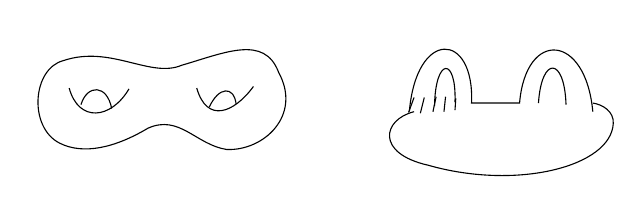
\begin{tikzpicture}[x=1cm,y=1cm]
\draw (0,0) .. controls (-.4,.2) and (-.35,.95) .. (.05,1.05)
.. controls (.65,1.25) and (1.15,.82) .. (1.55,.99)
.. controls (2.1,1.15) and (2.6,1.38) .. (2.78,.9)
.. controls (3.08,.35) and (2.59,-.1) .. (2.12,-.08)
.. controls (1.73,-.02) and (1.52,.37) .. (1.12,.19)
.. controls (.7,-.06) and (.3,-.15) .. (0,0);
\draw (.12,.7) .. controls (.24,.26) and (.65,.3) .. (.88,.69);
\draw (.27,.49) .. controls (.35,.75) and (.6,.75) .. (.66,.44);
\draw (1.74,.7) .. controls (1.87,.25) and (2.21,.38) .. (2.46,.72);
\draw (1.9,.46) .. controls (2.02,.72) and (2.21,.73) .. (2.24,.5);
\draw (4.5,.4) .. controls (4.1,.3) and (4.01,-.13) .. (4.68,-.28)
.. controls (5.8,-.6) and (7,-.3) .. (7.03,.25)
.. controls (7.04,.4) and (6.9,.49) .. (6.77,.51);
\draw (4.44,.4) .. controls (4.53,1.46) and (5.27,1.42) .. (5.23,.51)
-- (5.84,.51) .. controls (5.92,1.45) and (6.68,1.4) .. (6.77,.4);
\draw (4.76,.47) .. controls (4.77,1.1) and (5.04,1.1) .. (5.02,.52);
\draw (6.08,.51) .. controls (6.12,1.11) and (6.41,1.1) .. (6.43,.49);
\draw (4.43,.39)--(4.5,.58);
\draw (4.58,.38)--(4.63,.58);
\draw (4.74,.4)--(4.78,.59);
\draw (4.88,.4)--(4.9,.59);
\draw (5.02,.42)--(5.03,.57);
\end{tikzpicture}
\end{adjustbox}

На $\forall$ поверхности есть соотв. модель CFT!!

\SourceFigure{GELFAND-P001480}{middle-cut-torus}{Разрезанный тор: два близких овальных торца внизу, подпись $\theta$ под разрезом, подпись $\beta$ наверху. Внутри видна изогнутая линия и плотный штрих у левого внутреннего края; различение стрелки и линии поверхности неуверенно.}
$$
=f(\beta+i\theta,\beta-i\theta)\qquad
\text{(вещ. аналит. ф-и)}
$$
можно подкрутить по $\theta$

Параметры тора — 2 вещ. числа
$$\tau=L+i\theta$$

\begin{adjustbox}{max width=\linewidth}
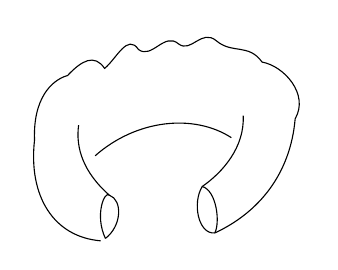
\begin{tikzpicture}[x=1cm,y=1cm]
\draw (.7,0) .. controls (.1,.05) and (-.22,.57) .. (-.14,1.28)
.. controls (-.16,1.8) and (.07,2.04) .. (.28,2.1)
.. controls (.46,2.29) and (.62,2.38) .. (.75,2.19)
.. controls (.9,2.31) and (1.04,2.64) .. (1.18,2.43)
.. controls (1.35,2.3) and (1.51,2.66) .. (1.69,2.5)
.. controls (1.85,2.38) and (1.98,2.7) .. (2.17,2.54)
.. controls (2.37,2.37) and (2.58,2.51) .. (2.75,2.27)
.. controls (3.03,2.22) and (3.35,1.86) .. (3.17,1.55)
.. controls (3.11,.85) and (2.71,.36) .. (2.15,.1);
\draw (.76,.03) .. controls (.97,.19) and (.98,.52) .. (.81,.58)
.. controls (.75,.64) and (.62,.33) .. (.76,.03);
\draw (2.15,.1) .. controls (1.94,.08) and (1.86,.48) .. (1.99,.69)
.. controls (2.17,.64) and (2.22,.24) .. (2.15,.1);
\draw (.81,.58) .. controls (.48,.87) and (.38,1.18) .. (.42,1.47);
\draw (.63,1.08) .. controls (1.15,1.54) and (1.88,1.62) .. (2.36,1.31);
\draw (1.99,.69) .. controls (2.25,.87) and (2.53,1.19) .. (2.51,1.59);
\end{tikzpicture}
\end{adjustbox}

\begin{adjustbox}{max width=\linewidth}
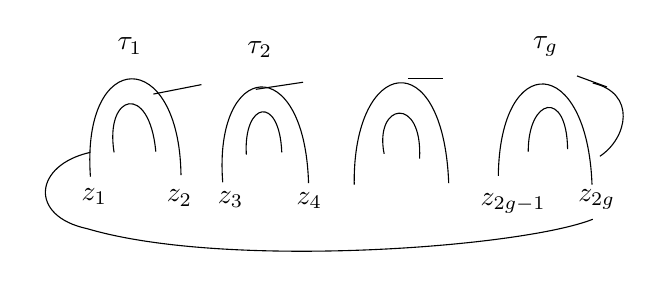
\begin{tikzpicture}[x=1cm,y=1cm]
\draw (0,.45) .. controls (-.72,.29) and (-.79,-.36) .. (-.04,-.52)
.. controls (1.72,-1.04) and (5.47,-.76) .. (6.38,-.4);
\draw (6.47,.4) .. controls (6.82,.63) and (6.94,1.2) .. (6.38,1.33);
\draw (.8,1.19)--(1.41,1.31);
\draw (2.1,1.25)--(2.7,1.34);
\draw (4.03,1.39)--(4.48,1.39);
\draw (6.18,1.42)--(6.56,1.28);
\draw (0,.14) .. controls (-.12,1.79) and (1.13,1.8) .. (1.15,.16);
\draw (.3,.45) .. controls (.18,1.2) and (.75,1.34) .. (.83,.46);
\draw (1.68,.07) .. controls (1.56,1.62) and (2.72,1.75) .. (2.77,.06);
\draw (1.98,.42) .. controls (1.94,1.09) and (2.4,1.19) .. (2.43,.45);
\draw (3.35,.04) .. controls (3.33,1.66) and (4.48,1.86) .. (4.55,.06);
\draw (3.73,.43) .. controls (3.6,1.08) and (4.22,1.18) .. (4.18,.37);
\draw (5.18,.15) .. controls (5.2,1.75) and (6.31,1.7) .. (6.37,.04);
\draw (5.56,.46) .. controls (5.56,1.14) and (6.05,1.26) .. (6.06,.49);
\node at (.5,1.8) {$\tau_1$};
\node at (2.15,1.76) {$\tau_2$};
\node at (5.78,1.79) {$\tau_g$};
\node at (.05,-.11) {$z_1$};
\node at (1.13,-.13) {$z_2$};
\node at (1.78,-.15) {$z_3$};
\node at (2.78,-.16) {$z_4$};
\node at (5.37,-.2) {$z_{2g-1}$};
\node at (6.43,-.15) {$z_{2g}$};
\end{tikzpicture}
\end{adjustbox}

важны длины и повороты подкрутки ручек (handles)
$$
\begin{array}{ccc}
0&1&\infty\\
\uparrow&\uparrow&\uparrow\\
z_1&z_2&z_3
\end{array}
$$
Получ. $3g-3$ компл. параметра.\qquad $(g\ge2)$
$$f(z_i,\tau_i;\bar z_i,\bar\tau_i)$$

\Unclear{GELFAND-P001480}{bottom-point-pair}{$(z_{2j-1},z_{2j})$ или $(z_{j-1},z_{2j})$ или $(z_{2j+1},z_{2j})$}
— точки, в к-рые
[зачёркнуто: \Unclear{GELFAND-P001480}{bottom-cancelled-word}{неразборчивое слово перед «приклеив.»}]
приклеив. ручки (тонкие)

$\tau_j$ — как в торе.

\SourcePage{GELFAND-P001481}{85}
\SourceFigure{GELFAND-P001481}{top-cft-sets}{Внешний овал с надписью CFT's; внутри меньший овал с надписью RCFT's. Под ним ISING, от этой надписи вверх проходит линия, оканчивающаяся в малом овале около маленького крестика или наконечника. Точная форма последнего знака неуверенна.}

R — Rational

I [зачёркнуто: \Unclear{GELFAND-P001481}{rational-cancelled-prefix}{неразборчивые буквы после I}]
\underline{RATIONAL.}\qquad (назв. — историческое)
$$
f(z_i,\tau_i,\bar z_i,\bar\tau_i)
=\sum_{j=1}^{N<\infty}\mathcal F_j(z_i,\tau_i)
\overline{\mathcal F}_j(\bar z_i,\bar\tau_i)
$$

\underline{Тор:}
$$\theta\to\theta+2\pi$$
$$\mathcal F_j(\tau)\ne\mathcal F_j(\tau+2\pi i)$$
$$\mathcal F_j(\tau)=\sum_\ell M_{j\ell}\mathcal F_\ell(\tau+2\pi i)$$
\Unclear{GELFAND-P001481}{torus-period-convention}{В обеих строках написано $\tau+2\pi i$; внизу этой страницы написано $T:\tau\to\tau+1$.}

$M=$ monodromy matrix.
[зачёркнуто: \Unclear{GELFAND-P001481}{monodromy-cancelled-word}{неразборчивое слово}]

E.g. Ising
$$
Z(\tau,\bar\tau)=
\left|\sqrt{\frac{\theta_2}{\eta}}\right|^2+
\left|\sqrt{\frac{\theta_3}{\eta}}\right|^2+
\left|\sqrt{\frac{\theta_4}{\eta}}\right|^2
$$
$$\sqrt{\frac{\theta_2}{\eta}}=q^{1/8}\prod(1+q^n),\qquad q=e^{2\pi i\tau}$$
$$\sqrt{\frac{\theta_3}{\eta}}=\prod(1-q^{n-1/2})$$
$$\sqrt{\frac{\theta_4}{\eta}}=\prod(1+q^{n-1/2}).$$
\Unclear{GELFAND-P001481}{ising-product-conventions}{Показатель $1/8$, знак минус в строке $\theta_3$ и знак плюс в строке $\theta_4$ воспроизведены по источнику; нормировка не уточнена.}

\underline{И.М.Г.} Эллиптич. ф-и — это тригонометрия с параметром $q$.

$\mathcal F_j$ — не инвариантны, но $f$ уже инвариантно

($\overline{\mathcal F}_j$
не обязательно компл. сопряжены к $\mathcal F_j$!)

Возникает группа кос.

\begin{adjustbox}{max width=\linewidth}
\begin{tikzpicture}[x=1cm,y=1cm]
\draw (0,.4) .. controls (-.25,1.06) and (.7,1.2) .. (1.2,1.13)
.. controls (1.75,1.02) and (2.55,1.53) .. (2.78,.92)
.. controls (3.16,-.12) and (2.33,-.29) .. (1.58,-.05)
.. controls (.89,.05) and (.12,.33) .. (0,.4);
\draw (.41,.57) .. controls (.14,.9) and (.87,1.02) .. (.98,.73)
.. controls (1.02,.49) and (.6,.47) .. (.41,.57);
\draw (2.06,.5) .. controls (1.65,.66) and (2.29,1.14) .. (2.43,.88)
.. controls (2.5,.63) and (2.23,.42) .. (2.06,.5);
\draw (.63,.49) .. controls (.84,.45) and (.79,.24) .. (.55,.24);
\draw (2.11,.44) .. controls (2.33,.58) and (2.53,-.07) .. (2.25,-.14)
.. controls (2.12,-.19) and (2.03,-.1) .. (2.05,.06);
\end{tikzpicture}
\end{adjustbox}

Generalize.

$g=1$
\begin{adjustbox}{max width=\linewidth}
\begin{tikzpicture}[x=1cm,y=1cm]
\draw (0,0) ellipse (1.1cm and .56cm);
\draw (-.48,.21) .. controls (-.57,-.12) and (.2,-.25) .. (.53,.22);
\draw (-.28,.01) .. controls (-.02,.22) and (.2,.16) .. (.29,-.02);
\draw (.12,-.12) .. controls (.5,-.2) and (.33,-.61) .. (.08,-.51)
.. controls (-.02,-.47) and (.01,-.22) .. (.12,-.12);
\end{tikzpicture}
\end{adjustbox}
$$
S:\tau\to-1/\tau\qquad
T:\tau\to\tau+1
$$
$$S^2=1,\qquad (ST)^3=I$$

\SourcePage{GELFAND-P001482}{unlabelled}
\underline{``DEHNTWIST''}

\underline{$g=2$}
\SourceFigure{GELFAND-P001482}{top-genus-two-twists}{Двуручная поверхность с кривыми и подписями $\alpha_1,\beta_1$ у левой ручки, $\alpha_2$ вдоль средней части и $\beta_2,\alpha_3$ у правой ручки. Часть кривых перекрывает края отверстий; разрывы и соединения штрихов не позволяют уверенно восстановить все прохождения.}
$$z_i,\tau_i\to\tilde z_i,\tilde\tau_i$$

$$\alpha_1\beta_1\alpha_1=\beta_1\alpha_1\beta_1$$
$$\alpha_2\beta_2\alpha_2=\beta_2\alpha_2\beta_2$$
$$\alpha_2\beta_1\alpha_2=\beta_1\alpha_2\beta_1\qquad(\beta_1\to\beta_2)$$
$$\alpha_1\alpha_2=\alpha_2\alpha_1$$
$$\beta_1\beta_2=\beta_2\beta_1\qquad\text{etc.}$$
$$ (\alpha_1\beta_1\alpha_2)^4=\alpha_3^2 $$
$$ (\alpha_3\beta_2\alpha_2\beta_1\alpha_1^2\beta_1\alpha_2\beta_2\alpha_3)^2=1 $$
$$ \beta_1^{-1}\alpha_1\beta_1=\alpha_1\beta_1\alpha_1^{-1}. $$

[Две горизонтальные черты с точкой между ними.]

CFT.
$$\mathcal A=\{(\sigma,\Delta)\ \text{fields}\}=\text{operator algebra}$$
$$\mathcal A\qquad\{T(z),T'(z),\ldots\}$$
$$
\mathcal H=\bigoplus_{i=1}^{N}
\underset{\mathcal A}{\mathcal H_i}\otimes
\underset{\bar{\mathcal A}}{\mathcal H_{\bar i}}
$$
$$\Delta:\mathcal A\to\mathcal A\otimes\mathcal A$$
$$ L_n=\oint_c\zeta^{n+1}T(\zeta) $$
$$ \to\oint\zeta^{n+1}T(\zeta)\otimes1+1\otimes\oint\zeta^{n+1}T(\zeta) $$
\Unclear{GELFAND-P001482}{ln-integration-symbol}{Буква переменной похожа на $\zeta$ или $\xi$; под первым контурным интегралом $c$ или $C$. Дифференциал в этих строках не написан.}

$\rho_i:\mathcal A\to\operatorname{End}\mathcal H_i$,\qquad
\Unclear{GELFAND-P001482}{rho-trailing-fragment}{$\rho_i\,C$ или $\rho_i\,O$; короткий фрагмент без видимого продолжения}

[Разделительная строка из мелких штрихов.]

\begin{adjustbox}{max width=\linewidth}
\begin{tikzpicture}[x=1cm,y=1cm]
\draw (0,0) .. controls (.08,.76) and (.27,1.6) .. (.48,2.1);
\draw (1.04,-.17) .. controls (1.49,.49) and (1.99,1.36) .. (2.03,2.05);
\draw (0,0) .. controls (.25,.2) and (.72,.06) .. (.9,-.08);
\draw (.49,.39)--(.85,1.77);
\draw[->] (.69,1.1)--(.85,1.77);
\draw[->] (.29,.75)--(1.41,.58);
\node at (1.01,1.8) {$\tau$};
\node at (1.59,.74) {$\sigma$};
\end{tikzpicture}
\end{adjustbox}
$$
S=\int g_{\mu\nu}(X)
[(\partial_\sigma X^\mu)(\partial_\sigma X^\nu)
-(\partial_\tau X^\mu)(\partial_\tau X^\nu)]
$$
Conformal Invariance $\to R_{\mu\nu}=0$.

\SourcePage{GELFAND-P001483}{86}

\underline{И.М.Г.} Что должно заменить понятие пр-ва при квантовании?

(планковская длина есть $\sim 10^{-33}$ м)
\Unclear{GELFAND-P001483}{planck-unit}{Единица после $10^{-33}$: м.}

\underline{1 вар.}: нечто дискретное.

Риман понимал, что это важно, и продумывал понятие пр-ва.

Тонкая пленка около 4-мерной поверхности.

\underline{Разумное упр.}: наивная геометрия 4-мерных многогранников.

\begin{center}
\begin{adjustbox}{max width=\linewidth}
\begin{tikzpicture}[x=1cm,y=1cm]
\draw (0,0) -- (0.75,-0.03);
\draw (1.07,0.01) -- (1.04,-0.12);
\draw (1.43,0.01) -- (2.47,-0.04);
\end{tikzpicture}
\end{adjustbox}
\end{center}

$$
S=\int_{R^4}g_{\mu\nu}(X)
\bigl[(\partial_\sigma X^\mu)(\partial_\sigma X^\nu)
-(\partial_\tau X^\mu)(\partial_\tau X^\nu)\bigr]+S_K
$$

[Под интегральным членом фигурная скобка; под ней и справа:]
$$
\begin{array}{ccc}
c_{R^4}&+c_K=&26\\
\Vert&&\\
4&&
\end{array}
$$

[От $S_K$ короткая черта к помете:]
компактный
\Unclear{GELFAND-P001483}{sk-annotation}{конд. на утолщ. пр-ва / конд. на уплотн. пр-ва / конд. на уполщ. пр-ва / конд. на уплощ. пр-ва}

можно заменить на $\forall$ другую модель с нек-рыми
св-вами инвариантности

$$
c\left(\begin{gathered}\text{conformal Field}\\\text{Theory}\end{gathered}\right)\text{ — }?
$$

[Под «Theory» короткая вертикальная черта и помета «любая»;
к «любая» снизу проведена фигурная линия от пометы слева «тоже им. смысл.».]

Поэтому [зачеркнуто:
\Unclear{GELFAND-P001483}{cft-cancellation}{имеет / имеют}]
это интересно.

\underline{19.9.88 г.}\qquad\underline{Сем. Гельфанда.}

\underline{\underline{Морозов А.}}

\underline{Конформная теория поля}
(по мотивам докл. Мура).

Теория струн развивается с 1984 года.

\underline{Исходная картинка}

\begin{center}
\begin{adjustbox}{max width=\linewidth}
\begin{tikzpicture}[x=1cm,y=1cm]
\draw (0,2.14) .. controls (0.24,2.25) and (0.32,1.97) .. (0.21,1.91)
 .. controls (0.03,1.80) and (0.37,1.71) .. (0.27,1.50);
\fill (0,2.14) circle (0.04);
\fill (0.27,1.50) circle (0.055);
\node[anchor=west] at (1.40,1.85) {в $R^{26}$};
\node[anchor=west] at (4.25,1.85) {$x^\beta,\quad\varphi(x)$ — поле};
\node[anchor=west] at (-0.05,0.83) {$x^\mu(\sigma)$};
\node[anchor=west] at (3.05,0.66) {$\Phi\{x_\mu(\sigma)\}$};
\node[anchor=west] at (6.25,0.66) {$\mu=1,\ldots,26$};
\node[anchor=west] at (-0.05,-0.23) {$\Phi\{C\}$};
\draw[->] (2.85,0.48) -- (1.60,-0.06);
\node[anchor=west] at (1.80,-0.35) {— ф-л от};
\end{tikzpicture}
\end{adjustbox}
\end{center}

\Unclear{GELFAND-P001483}{field-overwrite}{В строке «поле» знак перед $(x)$ переписан: $\varphi$ / $\Phi$.}
\Unclear{GELFAND-P001483}{contour-ending}{После «ф-л от»: контура / контуров; конец слова переписан.}

\begin{equation*}
(1)\quad
\langle\varphi(x_1)\ldots\varphi(x_n)\rangle
=\int D\varphi\,e^{\Sigma(\varphi)}\varphi(x_1)\ldots\varphi(x_n)
\end{equation*}

\Unclear{GELFAND-P001483}{eq1-first-symbol}{Первый знак поля в (1) переписан: $\varphi$ / $\Phi$.}

\SourceFigure{GELFAND-P001483}{particle-diagram}{Три линии с подписями $x_1$, $x_2$, $x_3$ слева. Верхняя линия волнистая; средняя и нижняя поднимаются вправо к двум местам на верхней линии. В первом месте темная точка; справа темная точка или наконечник. Точные соединения штрихов в этих местах неясны.}

(Вначале было 3 частицы, в конце ничего не осталось)

$\Sigma(\varphi)$ наз. квантовое действие

\SourcePage{GELFAND-P001484}{unlabelled}

Хотим то же в теор. струн

\begin{equation*}
(2)\quad
\langle\Phi(C_1)\ldots\Phi(C_n)\rangle
\longrightarrow
\int D\Phi\,e^{\Sigma(\Phi)}\Phi(C_1)\ldots\Phi(C_n);
\end{equation*}

\Unclear{GELFAND-P001484}{eq2-relation}{Переписанный знак перед интегралом: $\longrightarrow$ / $\Rightarrow$ / $=$.}

но в этом напр. никакого разумного прогресса нет!

Но: левую часть (2) можно опис. в других терминах.

\begin{equation*}
(3)\quad
\Phi(C)=\sum\varphi_n(x)e^{in\sigma}\qquad(\text{замкн. струна})
\end{equation*}

$\varphi_n$ — отожд. с полями в (1)

Рассмотрим

\begin{equation*}
(4)\quad
\langle\varphi_{N_1}(x_1)\ldots\varphi_{N_n}(x_n)\rangle
\end{equation*}

и для нее пишем другое предст.

\begin{equation*}
(5)\quad
\langle\varphi(x_1)\varphi(x_2)\rangle
=\int Dx\,e^{-mL},\qquad
L=\int\sqrt{\dot{x}^2}\,dt
\end{equation*}

\Unclear{GELFAND-P001484}{eq5-exponent-overwrite}{В показателе экспоненты буква после минуса переписана; видимое чтение $-mL$, первоначальные штрихи неразборчивы.}

[Под левой частью (5) вертикально поставленный знак равенства:]
$$
\begin{gathered}
\Vert\\
\int D\varphi\,e^{\Sigma_0(\varphi)}\varphi(x_1)\varphi(x_2)
\end{gathered}
$$

для [вставлено сверху: простейшего] действия $\Sigma_0$, опис. своб. частицу.

\begin{equation*}
(6)\quad
\Sigma_0(\varphi)=\int(\partial\varphi)^2\partial^{26}x
+\int\varphi^3d^{26}x
\end{equation*}

\Unclear{GELFAND-P001484}{eq6-measure}{Первый знак меры: $\partial$.}
\Unclear{GELFAND-P001484}{eq6-cubic-free}{Второе слагаемое: $+\int\varphi^3d^{26}x$.}

Теперь

\begin{equation*}
(7)\quad
\langle\varphi_{N_1}(x_1)\ldots\varphi_{N_n}(x_n)\rangle
\sim\int Dx\,e^S\,V_{N_1}(x)\ldots V_{N_n}(x),
\end{equation*}

[Под интегралом:]
по мир. поверхн. $x^\mu(\sigma,t)$
(несингулярным) и по всем топологиям

$V_{N_j}$ — вершинные операторы
\Unclear{GELFAND-P001484}{vertex-index}{Маленький нижний индекс при $N$: $j$ / $d$.}

(8)
\SourceFigure{GELFAND-P001484}{branching-diagram}{Лентовидная фигура: слева почти вертикальный край, сверху и снизу изогнутые границы до второй почти вертикальной черты. Справа расходятся четыре кривые; две внутренние пересекаются. Точное сопряжение границ со второй вертикальной чертой и значение пересечения неясны. Справа из области слова «ветвления» идет большая изогнутая стрелка влево к рисунку.}

Теор. струн: [зачеркнуто:
\Unclear{GELFAND-P001484}{branching-cancellation}{зап / запр}]
запрещены ветвления

\begin{center}
\begin{adjustbox}{max width=\linewidth}
\begin{tikzpicture}[x=1cm,y=1cm]
\node[anchor=east] at (-0.55,1.12) {(9)};
\draw (0.26,2.63) .. controls (0.87,2.93) and (1.64,2.65) .. (2.53,2.62)
 .. controls (3.63,2.57) and (4.75,2.61) .. (5.28,2.64);
\draw (0.08,2.43) .. controls (-0.14,2.65) and (0.13,2.75) .. (0.32,2.30)
 .. controls (0.40,2.04) and (0.34,0.85) .. (0.36,0.66);
\draw (5.27,2.64) .. controls (5.05,2.33) and (5.16,2.24) .. (5.40,1.98);
\draw (5.34,2.03) .. controls (4.47,1.97) and (3.03,1.95) .. (3.00,1.37)
 .. controls (2.96,1.02) and (4.51,1.05) .. (4.94,0.96)
 .. controls (5.14,0.94) and (5.35,0.78) .. (5.40,0.61);
\draw (5.48,0.66) -- (5.31,0.00);
\draw (0.18,0.44) .. controls (0.78,0.68) and (1.34,0.51) .. (1.76,0.47)
 .. controls (2.56,0.42) and (3.05,0.46) .. (3.55,0.26)
 .. controls (4.09,0.09) and (4.91,-0.12) .. (5.54,-0.03);
\end{tikzpicture}
\end{adjustbox}
\end{center}

(но такие превращ. остаются!)

и получается теория своб. частиц.


\SourcePage{GELFAND-P001485}{87}

\begin{equation*}
\int \mathcal{D}x\,e^{mL}
\longrightarrow
\int \mathcal{D}x\,\mathcal{D}\lambda\,
e^{\int \lambda^{-1}\dot{x}^{2}\,dt+\int m\lambda\,dt}
\tag{10}
\end{equation*}
[Перед $m\lambda\,dt$ зачёркнуто:
\Unclear{GELFAND-P001485}{eq10-cancellation}{неразборчивый знак, возможно $m$}.]

$L$ как в (5)

Интегрир. методом перевала справа (по $\lambda$), получаем
$\lambda^{2}=\dfrac{\dot{x}^{2}}{m^{2}}$.

\begin{equation*}
\int \mathcal{D}x\,e^{m\int\sqrt{\dot{x}^{2}}\,dx}
\tag{11}
\end{equation*}
\Unclear{GELFAND-P001485}{eq11-differential}{В конце показателя: $dx$; возможно $dt$.}

((11) $\Rightarrow$ (10) избавляет от корня). Оказ., что равенство точное!!

Число $\lambda$ имеет смысл 1-мерн. метрики
(всё остальное \Unclear{GELFAND-P001485}{metric-abbreviation}{свод. / своб.}
из репараметризации)

\begin{equation*}
\int\frac{d\lambda}{\lambda}\,e^{a\lambda}e^{b/\lambda}
=e^{\sqrt{ab}}
\tag{12}
\end{equation*}
\Unclear{GELFAND-P001485}{eq12-identity}{Равенство с $e^{\sqrt{ab}}$ без дополнительных множителей.}

Грин и др. сделали аналог. вещь в теор. струн: переход к

\begin{equation*}
\sum_{\text{топол.}}\int\mathcal{D}x\,\mathcal{D}g\,
e^{\int\sqrt{g}\,g^{ab}\partial_a x^{\mu}\partial_b x^{\mu}\,d\sigma\,dt}
\underbrace{e^{\int\sqrt{g}\,d\sigma\,dt}}_{\text{это можно убрать}}
\tag{13}
\end{equation*}

\underline{Обобщение:}

кривое 26-мерн. пр-во

\begin{equation*}
\begin{aligned}
\sum_{\text{топол.}}\int\mathcal{D}x\,\mathcal{D}g\,
e^{\int G_{\mu\nu}(x)\sqrt{g}\,g^{ab}\partial_a x^{\mu}\partial_b x^{\nu}}
&{}\\
&d\sigma\,dt
\end{aligned}
\tag{14}
\end{equation*}
\Unclear{GELFAND-P001485}{eq14-differentials}{Множитель $d\sigma\,dt$ написан ниже показателя экспоненты; принадлежность показателю неясна.}

Хотим, чтобы вып. ур-я Эйнштейна

\begin{equation*}
R_{\mu\nu}(x)=0
\tag{15}
\end{equation*}

\begin{equation*}
\begin{gathered}
(15)\ \Leftrightarrow\ \text{дилатационная инвариантность!}\\
\Downarrow\\
\text{ур-я Янга Миллса}
\end{gathered}
\end{equation*}

Все инвар. ур-я для высших полей — следствие дилат.
инвар. (в однопетлевом приближении)

\SourcePage{GELFAND-P001486}{unlabelled}

\underline{$26/\overline{\underline{\mathrm{IX}}}$-88 г.}
\qquad \underline{\underline{Сем. Гельфанда.}}

\underline{И.М.Г.} Читать кн. Фейнмана о КЭД и
\Unclear{GELFAND-P001486}{feynman-verb}{учить / учите / учиться}
\Unclear{GELFAND-P001486}{feynman-noun}{эстетике / эстетику}
у него.

Там КЭД изложена без ф-л — на одних картинках.

\underline{\underline{Казаков.}}
\quad \underline{Комбинаторика и новые раб. по струнам}

Произошли события (в комбинаторике)

\underline{Поляков} и
[зачёркнуто: \Unclear{GELFAND-P001486}{names-cancellation}{по?}]
\underline{Замолодчиков — Книжник — Поляков}
показали, что действит. модели, прив. выше, опис. 2-мерную
квант. гравитацию.

(Книжник — Поляков — Замолодчиков)

[Под именами:] по англ. алфавиту.

З.-К.-П. рассмотрели модель бозонной струны.

\begin{equation*}
S=\int d^{2}\xi\,\sqrt{g}\,\partial_a x^{\mu}\partial_b x^{\mu}\,g^{ab}
+\beta\int d^{2}\xi\,\sqrt{g}
\tag{1}
\end{equation*}

\begin{equation*}
Z(\beta)=\int\mathcal{D}g_{ab}\int\mathcal{D}x^{\mu}\,e^{-S}
\tag{2}
\end{equation*}

$\mu=1,\ldots,D$.

\SourceFigure{GELFAND-P001486}{metric-diagram}{Внизу справа две пересекающиеся примерно перпендикулярные оси: горизонтальная с подписью $\xi_1$ справа и вертикальная с подписью $\xi_2$ слева вверху. Справа от вертикальной оси, над горизонтальной, расположен замкнутый неровный контур, внутри которого написано $g_{ab}(\xi)$. Направления наконечников осей неуверенно различимы.}

\SourcePage{GELFAND-P001487}{unlabelled}

Интеграл (2) опр. при
\Unclear{GELFAND-P001487}{top-beta-inequality}{$\beta>\beta_c$ / $\beta\ge\beta_c$; знак переправлен}
и там ведёт себя как
\begin{equation*}
(\beta-\beta_c)^{2-\gamma_{\mathrm{str}}(D)}
\tag{3}
\end{equation*}

(в $\beta_c$ объём пов. стан. беск.)

[Над строкой: $\mathrm{str}=\mathrm{string}$.]

К.-П.-З. доказали, что
\begin{equation*}
\gamma_{\mathrm{str}}=\frac{1}{12}
\left(D-1-\sqrt{(D-1)(D-25)}\right).
\tag{4}
\end{equation*}

Это имеет смысл при
\Unclear{GELFAND-P001487}{upper-dimension-range}{$D\le1$ и $D\ge26$ [так в источнике]}.
Это получено с пом. алгебр Каца-Муди, возникших у исслед.
Лагранжиана.

\underline{Казаков и др.} предсказали неск. значений $\gamma_{\mathrm{str}}$:
при $D=-2,0,\frac12,1$

[На левом поле:
\Unclear{GELFAND-P001487}{left-margin-monogram}{ИГ / ИМ?}.]
Всё совпало!!

Определим:
\begin{equation*}
Z(\beta)=\sum_{n=0}^{\infty}e^{-2n\beta}Z_{2n},
\tag{5}
\end{equation*}
где $Z_n$ — число планарных графов
[вставлено над строкой: с $n$ вершинами]
с топологией сферы
(в вершине должны сход. 3 ребра)

Тогда
\begin{equation*}
Z(\beta)\sim(\beta-\beta_c)^{2-\gamma_{\mathrm{str}}(D)}
\tag{6}
\end{equation*}
[Над $\gamma_{\mathrm{str}}(D)$ проведена скобка; справа от неё: $=-\frac12$.]
Это соответствует $D=0$

\SourceFigure{GELFAND-P001487}{right-margin-triangle-graphs}{На правом поле два рисунка один под другим. В верхнем рисунке большой треугольник с верхней вершиной и горизонтальным основанием; внутри меньший треугольник той же ориентации. Каждая вершина внутреннего треугольника соединена с соответствующей внешней вершиной. На нижней стороне внутреннего треугольника около левой вершины есть утолщение, похожее на наконечник влево; у правой нижней внешней вершины есть штрихи, похожие на наконечник вправо. В нижнем рисунке внешний треугольник и три отрезка от его вершин к внутренней точке; отрезок от левой нижней вершины не вполне доходит до точки соединения двух других отрезков. Буквенных или числовых подписей у этих двух рисунков нет. Требуют проверки наконечники и смысл разрыва в нижнем рисунке.}

[Зачёркнуто:
\Unclear{GELFAND-P001487}{middle-cancelled-word}{число?}.]
Асимптотика
\begin{equation*}
Z_{2n}\sim\left(\frac{256}{27}\right)^n n^{-3+\gamma_{\mathrm{str}}}
\tag{7}
\end{equation*}

$\gamma_{\mathrm{str}}$ — универс. число, не зав. от способа опр. план. графов
(можно 4 ребра в 1 вершине и т. п.)

\underline{Формула для $Z_n$.}

[Перед оставленной правой частью (8) зачёркнута дробь:
\Unclear{GELFAND-P001487}{bottom-cancelled-fraction}{$2\frac{(4n+7)!}{(n-4)}$ / $2\frac{(4n+1)!}{(n-4)}$ / $2\frac{(4n-7)!}{(n-4)}$; $n$ либо $k$, факториал в знаменателе неясен}.]
\begin{equation*}
Z_{2k}=2\frac{(4k-3)!}{(3k-1)!\,k!}
\tag{8}
\end{equation*}
[Справа в (8) стоит множитель:
\Unclear{GELFAND-P001487}{bottom-final-factor}{$9^k$ / $g^k$}.]

$Z_{2k}$ — число планарных графов, впис. в $\Delta$-к с числом
внутр. вершин $=2k$.

\SourcePage{GELFAND-P001488}{91}

Tutte решил эту задачу чисто комбинаторно.

\SourceFigure{GELFAND-P001488}{top-triangle-graph}{Вверху слева нарисован внешний треугольник с верхней вершиной и почти горизонтальным основанием. Внутри меньший треугольник: около его верхней вершины подпись 1, около левой нижней — $i$, около правой нижней — 2. Внешние вершины соединены с соответствующими внутренними; ребро между внутренними вершинами 1 и 2 изогнуто. На левой стороне внешнего треугольника есть утолщение, похожее на направленный вниз наконечник. Неясно, обозначает ли оно стрелку или является наложением штрихов.}

Рассмотрим
\begin{equation*}
Z_n=\sum_{\substack{\text{графы}\\ \text{с }n\\ \text{верш.}}}
\int\prod_{i=1}^{n}d\vec{x}_i\,
e^{-\sum_{\langle ij\rangle}(x_i^{\mu}-x_j^{\mu})^2}
\tag{9}
\end{equation*}

$\langle ij\rangle$ — ближайшие соседи в графе;

внутр. вершины

(10) Интеграл в (9) равен $\det^{-D/2}(3I-G)$.

[От $G$ проведён штрих к пояснению:]
Матр. [зачёркнуто:
\Unclear{GELFAND-P001488}{middle-cancelled-incidence}{инцидентности?}]
смежности вершин

($G_{ij}=1\Longleftrightarrow i,j$ соед. ребром

$G_{ij}=0$
\Unclear{GELFAND-P001488}{middle-overdrawn-equivalence}{густо обведённый / зачёркнутый знак $\Longleftrightarrow$}
в прот. случае).

[В первой строке знак $G$ переправлен:
\Unclear{GELFAND-P001488}{middle-overdrawn-matrix-symbol}{прежний знак $E$ / $G$?}.]

\underline{\underline{Капранов Миша.}}

\underline{О раб. [зачёркнуто: Б.-Г.-Г.] о $\mathcal{D}$-модулях.}
[Под зачёркнутым сокращением вставлено: Берншт.-Гельф.-Гельф.]

$V$ — векторное [зачёркнуто:
\Unclear{GELFAND-P001488}{lower-cancelled-space-token}{пр / неразборчивый короткий знак}]
пространство, $P(V)$ — его проективизация.

$O(-1)$ — рассл. на $P(V)$ (основное);
[над «рассл.» вставлено: тавтологическое]

[Справа:]
\begin{equation*}
O(-1)\subset P(V)\times V
\end{equation*}
[Под $O(-1)$:
\Unclear{GELFAND-P001488}{lower-tautological-annotation}{два вертикальных дугообразных штриха: вертикальное равенство / двойная помета?},
справа от них $\{(\ell,x)\mid x\in\ell\}$.]

Точки $P(V)$ — это прямые $\ell$ в $V$, проход. через $0$;
она и явл. слоем над $\ell$.

$O(-k)=O(-1)^{\otimes k}$, $k>0$;

$O(+k)$ — двойств. расслоение к $O(-k)$.

\underline{Способ констр. новых расслоений:}

$\Lambda(V)$ — внешняя алгебра над $V$;

$\Lambda^k(V)$ — однородная степени $k$ часть $\Lambda(V)$.

Рассматриваются модули над $\Lambda(V)$ с градуировкой.
\begin{equation*}
\{\ldots\ M_{-1};\ M_0;\ M_1;\ \ldots\},
\qquad \Lambda^kM_i\subset M_{i+k}.
\end{equation*}

\underline{Упражнение к след. разу:} написать ответы для
[зачёркнуто:
\Unclear{GELFAND-P001488}{bottom-cancelled-exercise-symbol}{$M$ / $V$?}]
$\dim V=1$ и $2$.

\SourcePage{GELFAND-P001489}{unlabelled}
$V\ni v$, $v^2=0$ в $\Lambda(V)$.

Рассм. умножение на $v$:
\begin{equation*}
(1)\qquad
\ldots\to M_{-1}\overset{v}{\longrightarrow}M_0
\overset{v}{\longrightarrow}M_1\overset{v}{\longrightarrow}M_2\to\ldots
\end{equation*}
$v^2=0\ \Rightarrow$ получ. комплекс.
\begin{equation*}
\operatorname{Ker}v\supset\operatorname{Im}v,
\end{equation*}
[Зачёркнуто справа от формулы:
\Incomplete{GELFAND-P001489}{cancel-after-image}{Зачёркнутый фрагмент не удаётся прочесть.}]

Рассм. [Зачёркнуто:
\Incomplete{GELFAND-P001489}{cancel-before-bundle}{Зачёркнутый фрагмент между «Рассм.» и «расслоение» не удаётся прочесть.}]
расслоение
\begin{equation*}
v\longmapsto
\frac{\operatorname{Ker}\{v:M_0\to M_1\}}
{\operatorname{Im}\{v:M_{-1}\to M_0\}},\qquad v\ne0.
\end{equation*}
Это «расслоение», а точнее, «пучок» над $\mathbb P(V)$.

\underline{Примеры.}\newline
\underline{модулей}

1). Сам $\Lambda(V)$
\begin{equation*}
\underset{0}{\mathbb C}\overset{v}{\longrightarrow}
\underset{1}{V}\overset{v}{\longrightarrow}
\underset{2}{\Lambda^2V}\overset{v}{\longrightarrow}
\ldots\overset{v}{\longrightarrow}\underset{N}{\Lambda^NV}
\end{equation*}
Ей соотв. нулевое расслоение; $\operatorname{Ker}v=\operatorname{Im}v$.

2) Обрезанная алгебра $\Lambda$, т.е. $\Lambda^{\ge k}(V)$

(оставл. только компоненты степеней $\ge k$).
\begin{equation*}
\{0;\ \Lambda^kV\overset{v}{\longrightarrow}\Lambda^{k+1}V;\ \ldots\}
\end{equation*}
[Под стрелкой зачёркнут знак:
\Unclear{GELFAND-P001489}{truncated-arrow-cancel}{$v$ / $k$.}]

Расслоение:
\begin{equation*}
\operatorname{Ker}\{v:\Lambda^kV\to\Lambda^{k+1}V\}
=\Omega^{k-1}_{\mathbb P(V)}\otimes O(k)
\end{equation*}
[Под $\Omega^{k-1}_{\mathbb P(V)}$ проведена черта к подписи:
$(k-1)$-формы на $\mathbb P(V)$.]

3) Пусть $V$ — симплектич. пр-во, $[\ ,\ ]$ — $2$-форма;
[Над «$2$-форма» вписано и соединено фигурной скобкой:
\Unclear{GELFAND-P001489}{symmetry-note}{симм.}]

рассм. модуль
\begin{equation*}
0\to\underset{-1}{\mathbb C}\overset{v}{\longrightarrow}
\underset{0}{V}\overset{v}{\longrightarrow}\underset{1}{\mathbb C}\to0
\end{equation*}
\begin{equation*}
v:w\longmapsto[v,w]
\end{equation*}
\begin{equation*}
v\longmapsto v^{\perp}/\mathbb Cv,
\qquad\perp\text{ — ортог. отн. }[\cdot,\cdot]
\end{equation*}

\underline{Теорема.} Всякое алгебраическое векторное расслоение
над $\mathbb P(V)$ происходит у некоторого $\Lambda(V)$-модуля
\begin{equation*}
E=\frac{\operatorname{Ker}\{v:M_0\to M_1\}}
{\operatorname{Im}\{v:M_{-1}\to M_0\}},
\quad\text{а другие факторы }=0.
\end{equation*}

\SourcePage{GELFAND-P001490}{92}
\underline{Док-во} см. в приложении С. Гельфанда
к книге \underline{Оконек} и др. «Расслоения над проект. пр-вом».

\underline{Формулир.}: заметка в ФА в 1978 году.

В док-ве использ. \underline{производные} категории. Можно ли этого
избежать? С. Гельфанд считает, что нельзя.

\underline{Рез. Капранова}: описание рассл. над квадрикой
в $\mathbb P(V)$.
\begin{equation*}
V,\quad\langle\ \rangle,\qquad
\mathbb P(V)\supset Q=\{v:\langle v,v\rangle=0\}
\end{equation*}
[Под $\langle\ \rangle$ проведена черта к подписи: симм. форма.]

Строим град. ал. Клиффорда [Над строкой вписано со скобкой: $A(V)$],
порожд. образующими
\begin{equation*}
v,\quad\operatorname{deg}v=1\text{ и }h,\quad\operatorname{deg}h=2
\end{equation*}
[Под $h$ проведена черта к подписи: фиксир.]
\begin{equation*}
vv'+v'v=\langle v,v'\rangle h
\end{equation*}
В \Unclear{GELFAND-P001490}{basis-abbreviation}{ортон. / ортог.}
базисе $e_1,\ldots,e_r$
\Unclear{GELFAND-P001490}{clifford-normalization}{$e_i^2=h,\qquad
e_ie_k=-e_ke_i,\quad i\ne k.$}
При $r=3$ это $\approx$ кватернионы.

\begin{equation*}
\langle v,v\rangle=0\ \Rightarrow\ v^2=0
\end{equation*}
и строим такое же расслоение.

Тогда верна такая же теорема.



\end{document}
